\documentclass[11pt]{article}
% Shared preamble for stand-alone SDDS EPICS documents
% Defines common macros and margin settings.

% Hyperlink helper for program references
\newcommand{\progref}[1]{\hyperref[#1]{\texttt{#1()}}}

% Provide a no-op latexonly environment so html.sty is not required.
\newenvironment{latexonly}{}{}

% Equation environment used for requirements
\newenvironment{req}{\begin{equation}\mathrm{}}{\end{equation}}

% Consistent page layout
\pagestyle{plain}
\begin{latexonly}
  \tolerance=10000
\end{latexonly}
\setlength{\topmargin}{0.15 in}
\setlength{\oddsidemargin}{0 in}
\setlength{\evensidemargin}{0 in} % not applicable anyway
\setlength{\textwidth}{6.5 in}
\setlength{\headheight}{-0.5 in} % for 11pt font size
%\setlength{\footheight}{0 in}
\setlength{\textheight}{9 in}

\usepackage{latexsym,hyperref,sddstoolkit}
\usepackage[dvips]{graphicx}

\begin{document}

\title{User's Guide for SDDS-compliant EPICS Toolkit Version 5}
\author{L. Emery, M. Borland, H. Shang, R. Soliday\\Advanced Photon Source\\ \date{\today}}
\maketitle

The SDDS-compliant EPICS toolkit is a set of software applications for
the collection or writing of data in Experimental Physics and
Industrial Control System (EPICS) database records.  Though most of
the applications essentially do rather simple operations, the
combination of these and others from the SDDS postprocessing toolkit
allows arbitrarily complicated analysis of data and control of the
accelerators at the Advanced Photon Source. These tools are general
and can be applied to devices other than accelerators under control of
EPICS.

The EPICS tools presented here read and store data to SDDS-protocol
files.  SDDS (Self-Describing Data Set)\cite{SDDS_AP1.4} refers to a
particular implementation of a self-describing file protocol used at
APS. Self-describing means that the data is referred to and accessed by
name. Thus, a user doesn't need to know, say, in which column a piece
of tabular data is located. An ASCII header contains information about the
file's data structure, i.e. definitions of structure elements
such as columns (tabular data) and parameters (single values).

Initially adopted for complex physics simulation programs, it was clear
that the SDDS file protocol would excel in data-collecting software as
well. Typically, an EPICS tool would write EPICS data to an SDDS file with
each readback written to a column of name corresponding to the
EPICS database record name. Single value data that describe the experimental conditions
might be written to the file as parameters.
Once collected, the EPICS data can be further analyzed and plotted
with any of the SDDS tools described in \cite{SDDS_AP1.4}.
One can regard the EPICS tools as the layer between the EPICS
control system and more functional analyzing tools and scripts, with
SDDS protocol files as an intermediary.

Following conventional usage, EPICS database records will be referred
to as ``process variables'' or PVs in this manual.

\section{Manual Pages Overview}
\subsection{EPICS Toolkit Programs by Category}
\subsubsection{Configuration Save and Restore}
\begin{itemize}
  \item \progref{sddscasr} --- a new configuration save and restore program with many unique features.
  \item \progref{sddscaramp} --- Performs ramping of process variables between
the present state and the states in one or more SDDS files.
  \item \progref{toggle} --- Alternates between two sets of process variable values stored in snapshot files
        at a regular interval.
        Example application: Alternate between two configurations of an accelerator for debugging
        accelerator performance.
\end{itemize}

\subsubsection{Data Collecting}
\begin{itemize}
  \item \progref{cavget} --- Retrieves values of process variables using Channel Access or PVAccess.
  \item \progref{sddssnapshot} --- Reads values of process variables and writes them to a snapshot file.
        Example application: Taking successive sets of data.
  \item \progref{sddsmonitor} --- Reads values of process variables and writes them to a file at regular intervals.
        Example application: archiving of system performance, investigation of glitches.
  \item \progref{sddsglitchlogger} --- Reads values of process variables and writes them to a file or multifile at regular intervals when certain trigger occurs.
        Example application: archiving of system performance, inverstigation of
        transition-based, glitch-based and alarmed-based triggers.
  \item \progref{sddsvmonitor} --- Reads values of process variables
        and writes them to a file at regular intervals. The list of readback process
        variables is constructed by multiplying a rootname list and a suffix list.
        Example application: archiving of system performance, investigation of
        glitches.
  \item \progref{sddswmonitor} --- Reads values of waveform and scalar process variables and writes them to a file at regular intervals.
        Example application: archiving of system performance, investigation of glitches.
  \item \progref{sddsstatmon} --- Reads values of process variables, calculates statistics and writes them to a file at regular intervals.
        Example application: archiving of system performance.
  \item \progref{sddssynchlog} --- Reads values of process variables
        synchronously.  Example application: Analyze for correlations
        between various systems.
  \item \progref{sddsexperiment} --- Varies process variables and measures process variables,
        with optional statistical analysis.
        Example application:  investigation of unforeseen physical dependences,
        measure corrector-bpm response matrices.
  \item \progref{sddsvexperiment} --- Varies process variables and measures process variables,
        with optional statistical analysis. The list of readback process variables is
        constructed by multiplying a rootname list and a suffix list.  Example
        application: investigation of unforeseen physical dependences, measure
        corrector-bpm response matrices.
  \item \progref{sddsalarmlog} --- Collects alarm status of a list of process variables.
        Example applications: Logging alarms for a particular accelerator system over a period of
        many runs in order to compile a history of faults statistics.
  \item \progref{sddslogger} --- Reads values of process variables and writes them to a file at regular intervals. Similar to sddsmonitor but it generates less network traffic.
  \item \progref{sddslogonchange} --- Records only the values of process variables that change. This reduces the output file size if process variables do not change often.
\end{itemize}

\subsubsection{Control}
\begin{itemize}
  \item \progref{cavput} --- Sets values of process variables using Channel Access or PVAccess.
  \item \progref{cawait} --- Waits for process variables to satisfy specified conditions.
  \item \progref{sddscontrollaw} --- Reads a matrix for a control law-type equation and regulates the
values of a list of readback process variables by applying corrections to another list of process variables.
        Example application: removing slow drifts in accelerators (such as the energy of a linac beam), trajectory
        and orbit correction.
  \item \progref{squishPVs} --- Minimizes the absolute values of a set of readback process variables
        by varying setpoint process variables which have a physical influence on the readback process variables.
        Example application: Reducing the size of the trajectory in a beamline without knowledge of the
        response matrix between bpms and correctors.
  \item \progref{sddsoptimize} ---Minimizes or maximizes the RMS of a set of readback process variables by automatically varying setpoint process variables (or knobs composed of setpoint PVs), which have a physical influence on the readback process variables, through simplex or 1dscan method.
  \item \progref{sddspvtest} ---tests the process variable given by the inputfile are out-of-range or not and sets the number of out-of-range process variables to a control PV.
\end{itemize}

\subsection{Toolkit Program Usage Conventions}
(This text in this section is borrowed from \cite{SDDS_AP1.4}.)

In order to make the multitude of Toolkit programs easier to use, the
developers have attempted to use consistent commandline argument
styles.  The Toolkit programs all require at least one commandline
argument.  Therefore, if a program is executed without commandline
arguments, it is assumed that the user is asking for help.  In this
case, a help message is printed that shows syntax and (usually)
describes the meaning of the switches.  In general, program usage is
of the following form:\\
\hspace*{5mm}{\tt programName} {\em fileNames} {\em switches}.\\
Probably the simplest example would be \\
\hspace*{5mm}{\tt sddsquery } {\em fileName},\\
which would invoke {\tt sddsquery} to describe the contents of an SDDS file.
A slightly more complicated example would be\\
\hspace*{5mm}{\tt sddsquery } {\em fileName} {\tt -columnList},\\
which invokes {\tt sddsquery} to list just names of columns in a file.

Programs assume that any commandline argument beginning with a minus sign ('-') is an option; all others are
assumed to be filenames.  Note that case is ignored in commandline switches.  The specific meaning of a
filename is dictated by its order on the commandline.  For example, if two filenames are given, the first
would commonly be an input file while the second would commonly be an output file.

In some cases, a command with a single filename implies replacement of the existing file.  For example,\\
\hspace*{5mm}{\tt sddsconvert} {\em fileName} {\tt -binary}\\
would replace the named file with a binary version of the same data.   This command is completely equivalent to\\
\hspace*{5mm}{\tt sddsconvert} {\tt -binary} {\em fileName} \\
That is, unlike many UNIX commands, the position of filenames relative to options is irrelevant.

One might also wish to make a new file, rather than replacing the existing file.  This could be done by\\
\hspace*{5mm}{\tt sddsconvert} {\tt -binary} {\em fileName} {\em fileName2} \\
Note that while the option may appear anywhere on the commandline, the order of the filenames is crucial to
telling the program what to do.

In following manual pages and in the program-generated help text, program usage is described using the following
conventions:
\begin{itemize}
  \item The first token on the commandline  is the name of the program.
  \item Items in square-brackets ({\tt []}) are optional.  Items not in square brackets are required.
  \item Items in curly-brackets ({\tt \{\}}) represent a list of choices.  The choices are separated by
a \verb+|+ character, as in\\
{\tt \{ {\em choice1} | {\em choice2} | {\em choice3} \}}
  \item Items in italics are descriptions of arguments or data that must be supplied by the user.  These items are not typed
literally as shown.
  \item Items in normal print are typed as shown, with optional abbreviation.  These are
usually switch keywords or qualifiers.  Any unique abbreviation is acceptable.
\end{itemize}

In addition to using files, most toolkit programs also take input from pipes, which obviates the need for temporary
files in many cases.  For those programs that support pipes, one can employ the {\tt -pipe} option.  This option
provides a good example of what options look like.  For example, one could do the following to test binary-ascii
conversion:\\
\hspace*{5mm}{\tt sddsconvert -binary -pipe=out {\em fileName} \verb+|+ sddsconvert -ascii -pipe=in {\em fileName1} }\\
The {\tt -pipe=out} option to {\tt sddsconvert} tells it to deliver its output to a pipe; it still
expects a filename for input.  Similarly, the {\tt -pipe=in} option to {\tt sddsquery} tells it to
accept input from a pipe.

The {\tt -pipe} switch may be given in one of five forms: {\tt -pipe}, {\tt -pipe=input,output}, {\tt
-pipe=output,input}, {\tt -pipe=input}, {\tt -pipe=output} .  The first three forms are equivalent.  In a usage
message, these forms would be summarized as {\tt -pipe[=input][,output]}.  One could also use abbreviations like
{\tt -pipe=i}, {\tt -pipe=i,o}, etc.  For convenience in the manual, the data stream from or to a pipe will
often be referred to by the name of the file for which it substitutes.  Note that you may not deliver more
than one file on the same pipe.

\section{Manual Pages}
\label{ManualPages}
%
% cavget documentation.
%
\begin{sddsprog}{cavget}
\item \textbf{description:}
\verb+cavget+ retrieves values of one or more EPICS process variables using Channel Access or PVAccess.
It supports formatting, repeated acquisition and statistical analysis for scripting and data collection.
\item \textbf{examples:}
\begin{flushleft}{\tt
cavget -list=my:pv\\
cavget -repeat=number=10,pause=1 -labeled -list=quadrupole:current\\
cavget -statistics=number=100,pause=0.1,format=SDDS,file=stats.sdds -list=cavit:readback
}\end{flushleft}
\item \textbf{synopsis:}
\begin{flushleft}{\tt
usage: cavget [-list=<string>[=<value>][,<string>[=<value>]...]]\
[-range=begin=<integer>,end=<integer>[,format=<string>][,interval=<integer>]]\
[-floatformat=<printfString>] [-charArray] [-delimiter=<string>] [-labeled]\
[-noQuotes] [-embrace=start=<string>,end=<string>] [-cavputForm]\
[-statistics=number=<value>,pause=<value>[,format=[tagvalue][pretty][SDDS,file=<filename>]]]\
[-pendIoTime=<seconds>] [-dryRun] [-repeat=number=<integer>,pause=<seconds>[,average[,sigma]]]\
[-numerical] [-errorValue=<string>] [-excludeErrors]\
[-despike[[neighbors=<integer>][,passes=<integer>][,averageOf=<integer>][,threshold=<value>]]]\
[-provider={ca|pva}] [-info] [-printErrors] pvname [...]
}\end{flushleft}
\item \textbf{switches:}
\begin{itemize}
  \item {\tt -list} --- Build PV names from components or explicit names.
  \item {\tt -range} --- Append integer ranges to PV prefixes.
  \item {\tt -floatformat} --- Set printf-style format for floating point numbers.
  \item {\tt -charArray} --- Print character arrays as strings.
  \item {\tt -delimiter} --- String used to separate values.
  \item {\tt -labeled} --- Prepend PV names to values.
  \item {\tt -noQuotes} --- Suppress quotes around string values.
  \item {\tt -embrace} --- Surround output with given start and end strings.
  \item {\tt -cavputForm} --- Format output suitable for input to \verb+cavput+.
  \item {\tt -statistics} --- Compute statistics over repeated readings.
  \item {\tt -pendIoTime} --- Maximum time to wait for connections.
  \item {\tt -dryRun} --- List PV names without fetching values.
  \item {\tt -repeat} --- Take multiple readings with optional pause.
  \item {\tt -numerical} --- Use numerical values for enumerations.
  \item {\tt -errorValue} --- Substitute a value if a read fails.
  \item {\tt -excludeErrors} --- Omit values if a read fails.
  \item {\tt -despike} --- Remove outliers using neighbors/passes settings.
  \item {\tt -provider} --- Select Channel Access (ca) or PVAccess (pva).
  \item {\tt -info} --- Show connection and data type information.
  \item {\tt -printErrors} --- Print errors without aborting.
\end{itemize}
\item \textbf{see also:}
\begin{itemize}
  \item \progref{cavput}
  \item \progref{cawait}
\end{itemize}
\item \textbf{author:} Michael Borland, Robert Soliday, ANL/APS.
\end{sddsprog}

\begin{sddsprog}{cavput}
\item \textbf{description:}
    cavput sends values to EPICS process variables using Channel Access or PVAccess. It supports vector puts, delta mode, ramping, and numerical or char array data modes, making it useful for scripting accelerator operations.
\item \textbf{examples:}
    Set all storage ring quadrupoles to zero.
    \begin{verbatim}
    cavput -list=S -range=begin=1,end=40,format=\%ld
      -list=AQ,BQ -range=begin=1,end=5 -list=:CurrentAI=0
    
\end{verbatim}
    Configure slow beam history for S1A BPMs and 4080 samples.
    \begin{verbatim}
    cavput -list=S:bpm -range=begin=1,end=40,format=\%ld -list=:SlowBh:
      -list=MI=0,sizeAO=4080,modeBO=1,enableBO=1
    
\end{verbatim}
\item \textbf{synopsis:}
    \begin{verbatim}
usage: cavput [-list=<string>[=<value>][,<string>[=<value>]...]]
      [-range=begin=<integer>,end=<integer>[,format=<string>][,interval=<integer>]]
      [-pendIoTime=<seconds>] [-dryRun] [-deltaMode[=factor=<value>]] [-ramp=step=<n>,pause=<sec>]
      [-numerical] [-charArray] [-blunderAhead[=silently]]
      [-provider=\{ca|pva\}]
    
\end{verbatim}
\item \textbf{switches:}
\begin{itemize}
  \item {\tt -list} --- Specify PV name components with optional values. Repeating
    \verb+-list+ concatenates the components to form each PV name, and
    forms like \verb+-list=:Set=5+ assign the value \verb+5+.
  \item {\tt -range} --- Generate PV names from a range. For example,
    \verb+-list=Q -range=begin=1,end=4,format=%02d -list=:Set=0+
    creates \verb+Q01:Set+ through \verb+Q04:Set+ with value \verb+0+.
  \item {\tt -pendIoTime} --- Maximum time to wait for connections and return values (default 1.0~s).
  \item {\tt -dryRun} --- Show PV names and values without sending to IOCs.
  \item {\tt -deltaMode} --- Treat values as deltas from current PV values; optional factor.
  \item {\tt -ramp} --- Ramp to the value in steps with an optional pause.
  \item {\tt -numerical} --- Force conversion to numeric mode.
  \item {\tt -charArray} --- Use string mode for char array PVs.
  \item {\tt -blunderAhead} --- Continue puts even if some PVs fail to connect; \verb|silently| suppresses errors.
  \item {\tt -provider} --- Select Channel Access ({\tt ca}) or PVAccess ({\tt pva}).
\end{itemize}
\item \textbf{author:} Michael Borland, Robert Soliday, ANL/APS.
\end{sddsprog}

% cawait.tex documentation for cawait utility
% template similar to others
\begin{sddsprog}{cawait}
\item \textbf{description:}
\verb+cawait+ monitors one or more EPICS process variables and waits until
user-specified conditions are met. Logical operations allow combining
conditions, and optional commands or subprocesses may be invoked when
events occur.
\item \textbf{examples:}
Wait for beam current to rise above 5~mA and echo a message:
\begin{flushleft}{\tt
cawait -waitFor=SR:current,above=5 -onEvent="echo beam reached 5"
}\end{flushleft}
Require two PVs to satisfy conditions simultaneously:
\begin{flushleft}{\tt
cawait -waitFor=SR:state,equalTo=1 -and -waitFor=SR:mode,equalTo=2
}\end{flushleft}
\item \textbf{synopsis:}
\begin{flushleft}{\tt
cawait [-interval=<seconds>] [-timeLimit=<seconds>] [-totalTimeLimit=<seconds>]\
 -waitFor=<PVname>[,lowerLimit=<value>,upperLimit=<value>][,equalTo=<value>][,sameAs=<string>][,above=<value>][,below=<value>][,changed][,monitor]\
 [{-and | -or | -not}]\
 [-repeat[=<number>]]\
 [-emit=event=<string>[,timeout=<string>][,end=<string>]]\
 [-preEvent=<command>]\
 [-onEvent=<command>]\
 [-postEvent=<command>]\
 [-onEnd=<command>]\
 [-subprocess=<command>[,event=<string>][,timeout=<string>][,end=<string>]]\
 [-pendIOTime=<seconds>]\
 [-noWarnings]\
 [-provider=\{ca|pva\}]
}\end{flushleft}
\item \textbf{switches:}
  \begin{itemize}
  \item {\tt -interval} --- seconds between checks (default 0.1~s).
  \item {\tt -timeLimit} --- maximum time to wait for the condition.
  \item {\tt -totalTimeLimit} --- maximum total runtime.
  \item {\tt -waitFor} --- PV name and criterion for ending wait.
  \item {\tt -and}, {\tt -or}, {\tt -not} --- logical operations on previous results.
  \item {\tt -repeat} --- number of events to wait for (default~1; infinite if omitted).
  \item {\tt -emit} --- emit strings for events, timeouts, or end-of-run.
  \item {\tt -preEvent}, {\tt -onEvent}, {\tt -postEvent}, {\tt -onEnd} --- commands to execute before, during, after events, or at end.
  \item {\tt -subprocess} --- run a subprocess and send event/timeout/end messages.
  \item {\tt -pendIOTime} --- time allowed for channel access operations (default 10~s).
  \item {\tt -noWarnings} --- suppress timeout warnings.
  \item {\tt -provider} --- choose channel access ({\tt ca}) or PVAccess ({\tt pva}) provider.
  \end{itemize}
\item \textbf{author:} M. Borland, R. Soliday, ANL/APS.
\end{sddsprog}


% degauss: configure and trigger magnet degaussing cycles.
\begin{sddsprog}{degauss}
\item \textbf{description:}
\verb+degauss+ reads an SDDS specification file listing magnets and degaussing parameters.
It configures the corresponding subroutine records and, unless otherwise requested, initiates
magnet degaussing cycles for each device.
\item \textbf{examples:}
To configure magnets without starting degaussing and later query their state:
\begin{flushleft}{\tt
  degauss -configure booster.sdds\\
  degauss -query booster.sdds
}\end{flushleft}
\item \textbf{synopsis:}
  \begin{flushleft}{\tt
    degauss [-q|-query|-c|-configure|-s|-stop]\\
    \phantom{degauss }[-p|-pend|-pendIoTime <seconds>] [--] <spec-file>
  }\end{flushleft}
\item \textbf{switches:}
  \begin{itemize}
    \item {\tt -q\,|\,-query} --- Print degaussing state of devices in {\tt spec-file}.
    \item {\tt -c\,|\,-configure} --- Configure records for degaussing but do not start.
    \item {\tt -s\,|\,-stop} --- Halt degaussing of devices in {\tt spec-file}.
    \item {\tt -p\,|\,-pend\,|\,-pendIoTime <seconds>} --- Maximum time to wait for Channel Access I/O.
  \end{itemize}
\item \textbf{author:} C. Saunders, J. Anderson, R. Soliday, H. Shang, ANL
\end{sddsprog}

% sdds2dfeedforward: apply two-dimensional feedforward tables to actuators.
\begin{sddsprog}{sdds2dfeedforward}
\item {\bf description:}
\verb+sdds2dfeedforward+ performs two-dimensional feedforward on process variables.
It sets one or more actuators according to a predetermined function of two readback
values.  The user supplies tables giving the actuator value as a function of two
readbacks.  Each table is provided as an SDDS page containing the columns
\verb+Readback1Value+, \verb+Readback2Value+, and \verb+ActuatorValue+.  Parameters
\verb+Readback1Name+, \verb+Readback2Name+, and \verb+ActuatorName+ specify the
corresponding process variables.  Optional parameters include
\verb+ReadbackChangeThreshold+ and \verb+ActuatorChangeLimit+.

\item {\bf examples:}
A basic invocation reads an SDDS table and applies it every ten seconds:
\begin{flushleft}{\tt
sdds2dfeedforward ID1Compensation.sdds -interval=10
}\end{flushleft}
where \verb+ID1Compensation.sdds+ might contain
\begin{flushleft}{\tt
Readback1Name = ID1:X \quad Readback2Name = ID1:Y \quad ActuatorName = S1B:H1:CurrentAO\\
 Readback1Value  Readback2Value  ActuatorValue\\
------------------------------\\
       150.000       0.000          0.000\\
       100.000      50.000          1.000\\
        50.000     100.000         10.000\\
}\end{flushleft}
\item {\bf synopsis:}
\begin{flushleft}{\tt
sdds2dfeedforward <inputfile>\
       [-controlLog=<rootname>]\
       [-interval=<real-value>] [-steps=<integer-value>]\
       [-verbose] [-dryRun] [-offsetOnly]\
       [-averageOf=<number>[,interval=<seconds>]]\
       [-advance=<seconds>]\
       [-testValues=<SDDSfile>]\
       [-runControlPV=string=<string>[,pingTimeout=<value>]]\
       [-runControlDescription=<string>]\
       [-CASecurityTest]\
       [-pendIOtime=<seconds>] [-infiniteLoop]
}\end{flushleft}
\item {\bf files:}
\begin{itemize}
  \item {\bf input file:} An SDDS file with parameters \verb+Readback1Name+,
  \verb+Readback2Name+, and \verb+ActuatorName+.  Optional parameters include
  \verb+ReadbackChangeThreshold+ and \verb+ActuatorChangeLimit+.  Required
  columns are \verb+Readback1Value+, \verb+Readback2Value+, and
  \verb+ActuatorValue+.
\end{itemize}
\item {\bf switches:}
    \begin{itemize}
        \item {\tt interval=<real-value>} --- Interval in seconds between corrections.
        \item {\tt steps=<integer-value>} --- Number of iterations before exiting.
        \item {\tt verbose} --- Print additional information.
        \item {\tt dryRun} --- Readbacks are read but actuators are not changed.
        \item {\tt offsetOnly} --- Offset tables using initial readback values so
               no change is made until a readback moves.
        \item {\tt averageOf=<number>[,interval=<seconds>]} --- Average multiple
               readings of each readback before computing corrections.
        \item {\tt advance=<seconds>} --- Advance readback values based on their
               ramp rate by the given number of seconds.
        \item {\tt testValues=<file>} --- SDDS file giving limits for PV tests that
               suspend feedforward when violated.
        \item {\tt runControlPV=string=<string>[,pingTimeout=<value>]} --- Use a
               run-control PV and optional ping timeout.
        \item {\tt runControlDescription=<string>} --- Description for the
               run-control record.
        \item {\tt CASecurityTest} --- Check Channel Access security before
               writing values.
        \item {\tt pendIOtime=<seconds>} --- Time to wait for Channel Access
               operations.
        \item {\tt infiniteLoop} --- Run indefinitely.
        \item {\tt controlLog=<rootname>} --- Log input and output data to an
               SDDS file using the given root name.
    \end{itemize}
\item {\bf see also:}
  \begin{itemize}
    \item \progref{sddsfeedforward}
  \end{itemize}
\item {\bf author: M. Borland, ANL}
\end{sddsprog}

% sddsalarmlog: log changes of alarm status for specified process variables.
\begin{sddsprog}{sddsalarmlog}
\item \textbf{description:}
\verb+sddsalarmlog+ logs changes of alarm status for process variables named in an input file.
\item \textbf{examples:}
%
The status of the positron accumulator ring process variables are logged
for a one day duration.
\begin{verbatim}
sddsalarmlog PAR.along PAR.along.sdds -timeDuration=1,day
\end{verbatim}
where the file \verb+PAR.along+ is the input file containing the names of the
process variables, and the file \verb+PAR.along.sdds+ is the output file.

\item \textbf{synopsis:}
\begin{verbatim}
usage: sddsalarmlog <input> <output>
-timeDuration=<realValue>[,<time-units>] [-offsetTimeOfDay]
[-append[=recover] | -eraseFile | -generations[=digits=<integer>][,delimiter=<string>] |
 -dailyFiles[=verbose]]
[-pendEventTime=<seconds>] [-durations] [-connectTimeout=<seconds>]
[-explicit[=only]] [-verbose] [-comment=<parameterName>,<text>]
[-requireChange[=severity][,status][,both]]
[-inhibitPV=name=<name>,pendIOTime=<seconds>]
[-watchInput]
[-runControlPV=string=<string>,pingTimeout=<value>]
[-runControlDescription=string=<string>]
\end{verbatim}

\item \textbf{files:}
\begin{itemize}
  \item \textbf{input file:}\par
The input file is an SDDS file with the required string column {\tt ControlName}
which contains the names of the process variables whose status is to be monitored.

  \item \textbf{output file:}\par
The output file contains information on the process variable alarm status
change, such as the time of occurrence, the alarm designation, the severity of the alarm, and the
row location of the previous alarm status change.

In order to save disk space {\tt sddsalarmlog} logs integer codes
(indexes) instead of the actual string values for the control name,
the alarm status and the alarm severity. The integer codes are indices
into one of three string arrays written to the output file. The logging information
can be recovered using SDDS tool sddsderef.

As an option, and for a direct interpretation of the output file, the control
name, alarm status and alarm severity can be written explicitly as
string columns with or without the integer codes. However this
option uses up a lot more disk space.

In either case the following columns are defined:
  \begin{itemize}
    \item {\tt PreviousRow} --- Long column of row numbers. For each
        process variables alarm status change, the row location of the
        previous alarm status change is written.
    \item {\tt TimeOfDay} --- Float column of system time in units of hours.
        The time does not wrap around at 24 hours.
  \end{itemize}

By default these columns are defined (except when the option {\tt -explicit=only} is specified):
  \begin{itemize}
    \item {\tt ControlNameIndex} --- Long column indicating the process variable whose
        alarm status changed. The value of this data is the index into the string array
        {\tt ControlNameString}, which is the list of all process variables monitored.
    \item {\tt AlarmStatusIndex} --- Short column indicating the alarm status.
         The value of this data is the index into the string array
        {\tt AlarmStatusString}, which is the list of all possible alarm status values.
    \item {\tt AlarmSeverityIndex} --- Short column indicating the alarm status.
        The value of this data is the index into the string array
        {\tt AlarmSeverityString}, which is the list of all possible alarm severity values.
  \end{itemize}

These columns are created by the option {\tt -explicit}:
  \begin{itemize}
    \item {\tt ControlName} --- String column for the process variable whose alarm
        status just changed.
    \item {\tt AlarmStatus} --- String column for the alarm status.
    \item {\tt AlarmSeverity} --- String column for the alarm severity.
  \end{itemize}

This column is created with option {\tt -durations}:
  \begin{itemize}
    \item {\tt Duration} --- String column for the duration of the previous alarm state.
  \end{itemize}

These arrays are created by default except when the option {\tt -explicit=only} is specified:
  \begin{itemize}
    \item {\tt ControlNameString} --- String colunm of all process variables to be monitored.
    \item {\tt AlarmStatusString} --- String colunm of all possible alarm status values.
    \item {\tt AlarmSeverityString} --- String colunm of all possible alarm severity values.
  \end{itemize}

These parameters are defined:
  \begin{itemize}
    \item {\tt InputFile} --- String parameter for the name of the input file.
    \item {\tt TimeStamp} --- String parameter for time stamp for file.
    \item {\tt PageTimeStamp} --- String parameter for time stamp for each page. When data
                is appended to an existing file, the new data is written to a new
                page. The {\tt PageTimeStamp} value for the new page is the creation
                date of the new page. The {\tt TimeStamp} value for the new page is the creation
                date of the very first page.
    \item {\tt StartTime} --- Double parameter for start time from the {\tt C} time call cast to type double.
    \item {\tt YearStartTime} --- Double parameter for start time of present year from the {\tt C} time call cast to type double.
    \item {\verb+StartYear+} --- Short parameter for the year when the file was started.
    \item {\verb+StartJulianDay+} --- Short parameter for the day when the file was started.
    \item {\verb+StartMonth+} --- Short parameter for the month when the file was started.
    \item {\verb+StartDayOfMonth+} --- Short parameter for the day of month when the file was started.
    \item {\verb+StartHour+} --- Short parameter for the hour when the file was started.
  \end{itemize}
\end{itemize} % end of itemized files


\item \textbf{switches:}
\begin{itemize}
  \item {\tt -timeDuration=<realValue>[,<time-units>]} --- Specifies time duration for logging.
        The default time units are seconds; one may also specify days, hours, or minutes.
  \item {\tt -offsetTimeOfDay} --- Adjusts the starting \verb+TimeOfDay+ value so it corresponds to the day for which most data is taken.
  \item {\tt -append[=recover]} --- Specifies appending to the file \verb+<output>+ if it exists already.
        If the \verb+recover+ qualifier is given, recovery of a corrupted file is attempted using \verb+sddsconvert+.
  \item {\tt -eraseFile} --- If the output file already exists, then it will be overwritten.
  \item {\verb+-generations[=digits=<integer>][,delimiter=<string>]+} ---
        Sends output to \verb+<output>-<N>+, where \verb+<N>+ is the smallest positive integer such that the file does not already exist.
        By default, four digits are used for formatting \verb+<N>+.
  \item {\tt -dailyFiles[=verbose]} --- Uses daily generation filenames of the form \verb+<output>-YYYY-JJJ-MMDD.<N>+.
        If \verb+verbose+ is given, a message is printed when a new file is started.
  \item {\tt -pendEventTime=<seconds>} --- Specifies the CA pend event time in seconds. The default is 10.
  \item {\tt -durations} --- Includes state duration and previous row reference data in the output.
  \item {\tt -connectTimeout=<seconds>} --- Specifies maximum time in seconds to wait for a connection before issuing an error message.
        The default is 60.
  \item {\tt -explicit[=only]} --- Specifies that explicit columns with control name, alarm status, and alarm severity strings be output in addition to the integer codes.
        If the \verb+only+ qualifier is given, the integer codes are omitted.
  \item {\tt -verbose} --- Prints a message when data is taken.
  \item {\tt -comment=<parameterName>,<text>} --- Adds a comment parameter with the given text to the output file.
  \item {\tt -requireChange[=severity][,status][,both]} --- Requires the specified changes before an event is logged.
  \item {\tt -inhibitPV=name=<name>,pendIOTime=<seconds>} --- Checks this process variable periodically and aborts data collection if it is nonzero.
  \item {\tt -watchInput} --- Monitors the input file for modifications and exits if it changes.
  \item {\tt -runControlPV=string=<string>,pingTimeout=<value>} --- Specifies a run control PV name and optional ping timeout in seconds.
  \item {\tt -runControlDescription=string=<string>} --- Specifies a run control PV description record.
\end{itemize}

\item \textbf{see also:}

% replacing <prog> with the program to be referenced:

\item \textbf{author:} M. Borland, ANL
\end{sddsprog}

%
% Template for making SDDS Toolkit manual entries.
%
\begin{sddsprog}{sddsbcontrol}
\item {\bf description:}
\verb+sddsbcontrol+ monitors the ramp slope and zero offsets of booster magnet power supplies and applies corrections through control process variables. It runs continuously, loading new amplitudes as needed and optionally registers with the runControl system.

\item {\bf examples:}
Start the booster ramp control loop:
\begin{flushleft}{\tt
sddsbcontrol\\
}\end{flushleft}

\item {\bf synopsis:}
\begin{flushleft}{\tt
usage: sddsbcontrol\\
}\end{flushleft}

\item {\bf switches:} none

\item {\bf see also:} \progref{sddscontrollaw}, \progref{sddsfeedforward}

\item {\bf author: R. Soliday, ANL/APS}
\end{sddsprog}

%
% Documentation for sddscainfo
%
\begin{sddsprog}{sddscainfo}
\item \textbf{description:}
  \verb+sddscainfo+ reads a list of process variable (PV) names from an SDDS file,
  queries the control system for metadata, and writes the results to an SDDS output file.
  The program can also create input files for \progref{sddspvalogger} or \progref{sddspvasaverestore}.

\item \textbf{examples:}
  Gather connection information for the PVs listed in \verb+pvList.sdds+ and write the results to \verb+pvInfo.sdds+.
  \begin{flushleft}{\tt
sddscainfo pvList.sdds pvInfo.sdds
  }\end{flushleft}
  Create a metadata file and a corresponding input for \progref{sddspvalogger}.
  \begin{flushleft}{\tt
sddscainfo pvList.sdds pvInfo.sdds -makeLoggerInput
  }\end{flushleft}
  Create a metadata file and a corresponding input for \progref{sddspvasaverestore}.
  \begin{flushleft}{\tt
sddscainfo pvList.sdds pvInfo.sdds -makeSCRInput
  }\end{flushleft}

\item \textbf{synopsis:}
  \begin{flushleft}{\tt
sddscainfo [<inputfile>] [<outputfile>]\
[-pipe=[input][,output]]\
[-makeLoggerInput[=withStorageType]]\
[-makeSCRInput]\
[-verbose]\
[-pendIOTime=<seconds>]
  }\end{flushleft}

\item \textbf{files:}
\begin{itemize}
  \item \textbf{input file:} SDDS file with string column \verb|ControlName| listing PVs to query.
  \item \textbf{output file:} SDDS file containing metadata for each PV.
\end{itemize}

\item \textbf{switches:}
\begin{itemize}
  \item {\tt -pipe[=input][,output]} --- read from standard input and/or write to standard output.
  \item {\tt -makeLoggerInput[=withStorageType]} --- write an input file for \progref{sddspvalogger}; append \verb|withStorageType| to include the storage type.
  \item {\tt -makeSCRInput} --- write an input file for \progref{sddspvasaverestore}.
  \item {\tt -verbose} --- print PV metadata to the terminal.
  \item {\tt -pendIOTime=<seconds>} --- time to wait for Channel Access operations (default 0.5 s).
\end{itemize}

\item \textbf{see also:}
\begin{itemize}
  \item \progref{sddspvalogger}
  \item \progref{sddspvasaverestore}
\end{itemize}

\item \textbf{author:} R. Soliday, ANL
\end{sddsprog}

%
% Documentation for sddscaplayback
%
\begin{latexonly}
\newpage
\end{latexonly}

\subsection{sddscaplayback}
\label{sddscaplayback}

\begin{itemize}
\item {\bf description:}
\verb+sddscaplayback+ reads waveform data from a multi-page SDDS file and writes the values to
EPICS process variables at a fixed interval. Each page in the input file represents a set of
numerical values for a single PV, which may be sent either as absolute values or as differences
from the current value.

\item {\bf examples:}
The following command plays back the waveforms in \verb+orbit.sdds+ once with a half-second
interval between pages.
\begin{flushleft}{\tt
sddscaplayback orbit.sdds -interval=0.5 -mode=absolute -repetitions=1
}\end{flushleft}

\item {\bf synopsis:}
\begin{flushleft}{\tt
sddscaplayback <inputFile> -interval=<seconds> [-repetitions=<number>]\\
-mode=\{absolute|differential\} [-triggerPV=<string>] [-controlNameParameter=<string>]\\
[-dataColumn=<columnName>] [-offset=<integer>] [-timeoffset=<seconds>]\\
[-factor=<value>] [-restore] [-verbose] [-pendIOtime=<seconds>]\\
[-runControlPV=string=<string>,pingTimeout=<value>]\\
[-runControlDescription=string=<string>]
}\end{flushleft}

\item {\bf files:}
The input file is an SDDS file containing a string parameter \verb+ControlName+ for the PV name
and a numerical column \verb+Value+ (or the column specified by \verb+-dataColumn+) for the
waveform data. Each page corresponds to a different PV.

\item {\bf switches:}
  \begin{itemize}
  \item {\tt -interval=<seconds>} --- Interval between sending pages.
  \item {\tt -repetitions=<number>} --- Number of times to loop through pages; default is infinite.
  \item {\tt -mode=\{absolute|differential\}} --- Send values directly or as differences from starting values.
  \item {\tt -triggerPV=<string>} --- PV that restarts playback when it changes.
  \item {\tt -controlNameParameter=<string>} --- Name of parameter holding PV names; defaults to {\tt ControlName}.
  \item {\tt -dataColumn=<columnName>} --- Column containing waveform data; defaults to {\tt Value}.
  \item {\tt -offset=<integer>} --- Offset into pages used as circular buffer.
  \item {\tt -timeoffset=<seconds>} --- Fine time offset less than the interval.
  \item {\tt -factor=<value>} --- Scale factor applied to waveform data.
  \item {\tt -restore} --- Restore PVs to starting values on exit.
  \item {\tt -verbose} --- Print status information.
  \item {\tt -pendIOtime=<seconds>} --- Channel access pend IO time.
  \item {\tt -runControlPV=string=<string>,pingTimeout=<value>} --- Enable run control monitoring.
  \item {\tt -runControlDescription=string=<string>} --- Description used with run control.
  \end{itemize}

\item {\bf see also:}
  \begin{itemize}
  \item \progref{sddslogger}
  \item \progref{sddscaramp}
  \item \progref{sddssnapshot}
  \end{itemize}

\item {\bf author: M. Borland, ANL}
\end{itemize}

% sddscaramp: ramp process variables between current and target states.
\begin{sddsprog}{sddscaramp}
\item \textbf{description:}
\verb+sddscaramp+ performs ramping of process variables between
the present state and the states in one or more SDDS files.

\item \textbf{examples:} 
% 
The following example shows how one would use \verb+sddscaramp+ to
ramp 50\% of the way to a new steering configuration, using 10
steps and pausing 1 second between steps: 
\begin{verbatim}
sddscaramp -rampTo=steering.snap,steps=10,pause=1,percentage=50
\end{verbatim}
The file \verb+steering.snap+ contains corrector magnet power supply
settings, such as might be saved to an SDDS file using the
\verb+sddssnapshot+ program.
\item \textbf{synopsis:} 
\begin{verbatim}
sddscaramp
  -rampTo=<filename>,steps=<number>,pause=<seconds>[,percentage=<value>][,differential=<factor>]
  [-rampTo ...] [-controlNameColumn=<string>] [-dataColumn=<columnName>]
  [-pendIOtime=<seconds>] [-resendFinal] [-verbose]
\end{verbatim}
\item \textbf{files:}

The input files are SDDS files.  There must be a string column named
{\tt ControlName}, {\tt Device}, or {\tt DeviceName} that contains the
process variable names.  There must also be a string column named {\tt
ValueString}, a numerical column named {\tt Value}, or a column of
either type with the name specified by the \verb+-dataColumn+ option;
this column contains the final value for the corresponding process
variable.  

When data is supplied in a string column, {\tt sddscaramp} needs a way
to determine if the data value is actually a number rather than a
literal string value (e.g., an enumerated value).  The optional {\tt
IsNumerical} column can be used for this purpose.  If supplied, this
column should contain character values {\tt y} or {\tt n}, indicating
that each PV (respectively) does or does not have numerical values.
If the {\tt IsNumerical} column does not exist or is not of character
type, then {\tt sddscaramp} uses an internal algorithm to decide
whether the data for each PV is numerical or not.  This may fail in
the case of enumerated values that contain numbers, resulting in
incorrectly restored values.  For reliable results, the use of {\tt
IsNumerical} with string data is required.  If the data is in a
numerical column to begin with, of course, there is no ambiguity.

\item \textbf{switches:}
    \begin{itemize}
        \item {\tt -rampTo={\em filename},steps={\em
        number},pause={\em seconds},[percentage={\em value}][,differential={\em factor}]} ---
        Specifies a file to ramp to, the number of steps in the ramp,
        and the time to wait between sending setpoints for each step.
        Optionally, one may specify ramping only part of the way to
        the configuration in the file or offsetting by a scaled
        amount using the {\tt differential} factor.  If several
        {\tt -rampTo} options are given, {\tt sddscaramp} ramps to each
        of them in the order given.
        \item {\tt -controlNameColumn={\em name}} --- Specifies the
        name of the column containing the PV names when it is not
        one of {\tt ControlName}, {\tt Device}, or {\tt DeviceName}.
        \item {\tt -dataColumn={\em name}} --- Specifies the name of
        the column in the input files that contains the PV values.
        By default, the program uses {\tt ValueString} or {\tt Value}.
        \item {\tt -pendIOtime={\em seconds}} --- Sets the time to
        wait for channel access operations to complete.
        \item {\tt -resendFinal} --- Resends the final setpoint for
        numerical PVs after ramping is complete.
        \item {\tt -verbose} --- If given, informational text is
        printed out as the ramping proceeds.
      \end{itemize}

\item \textbf{see also:}
    \begin{itemize}
% replacing <prog> with the program to be referenced:
    \item \progref{sddssnapshot}
    \item \progref{sddscasr}
    \end{itemize}
\item \textbf{author:} M. Borland (ANL)
\end{sddsprog}

%
% Template for making SDDS Toolkit manual entries.
%
\begin{latexonly}
\newpage
\end{latexonly}

%
% Substitute the program name for sddsmonitor
%
\subsection{sddscasr}
\label{sddscasr}

\begin{itemize}
\item {\bf description:}
%
% Insert text of description (typically a paragraph) here.
%
\verb+sddscasr+ is an alternative version of casave and carestore. sddscasr is
more efficient and has more features than casave/carestore. It can save
and restore configurations in one program.

\item {\bf example:} 
%
% Insert text of examples in this section.  Examples should be simple and
% should be proceeded by a brief description.  Wrap the commands for each
% example in the following construct:
% 
%
Save a snapshot of APS storage ring:
\begin{verbatim}
sddscasr SR.req SR.snapshot -save -pendIOTime=100
\end{verbatim}
Restore a snapshot:
\begin{verbatim}
sddscasr snapshot -restore -pendIOTime=100
\end{verbatim}
save snapshot with daemon mode, the output file in following command is out1-<current date and time>.
Whenever the value of casavePV (oag:casave) is changed to 1, a new saving starts and data is written
to a new output file with rootname of out1. (var1 is the input file contains PVs to be read)
\begin{verbatim}
sddscasr var1 out1 -runControlPV=string=oag:ControlLawRC 
-runControlDesc=string=test -daemon -daily -save -pidFile=pidFile
 -casavePV=oag:casave -logFile=logFile &
\end{verbatim}

\item {\bf synopsis:} 
%
% Insert usage message here:
%
\begin{verbatim}
usage: sddscasr <inputfile> <outputRoot> [-verbose]
    [-daemon] [-dailyFiles] [-semaphore=<filename>] [-save] [-restore] [-logFile=<filename>]
    [-runControlPV={string=<string>|parameter=<string>},pingTimeout=<value>,pingInterval=<value>]
    [-runControlDescription={string=<string>|parameter=<string>}] [-unique] [-outputFilePV=<pvname>]
    [-pidFile=<pidFile>] [-casavePV=<string>] [-interval=<seconds>] [-pipe=[input|output]]
    [-numerical] [-waveform=[rootname=<string>][,directory=<string>]]
    [-outputFilePV=<pvname>] [-casavePV=<string>]
\end{verbatim}
\item {\bf files:}
% Describe the files that are used and produced
\begin{itemize}
\item {\bf input file:} \par
The input file is an SDDS file with a string column. For saving snapshot, the input file
contains at least one string column - ControlName. For restoring snapshot, the input file
contains at least two string columns - ControlName and ValueString, where ValueString is the
value of the PVs to be restored.
\item {\bf output file:} \par
The output file only exists for saving snapshot. The output file contains everything in the input
file, except that the ValueString column (if the input file has ValueString column) is update. And
three more columns are created if they do not exist in the input file and their values are updated.
\begin{itemize}
\item {ValueString}: the values of the PVs given in the input file.
\item {IndirectName}: its value  is - for scalar PV or PVname for waveform PV.
\item {CAError}: its value is y if error occurred during channel access for
corresponding PV or n if no error occurs.
\end{itemize}
\end{itemize}

%
\item {\bf switches:}
%
% Describe the switches that are available
%
    \begin{itemize}
    \item {\tt inputFile} --- inputFile name (SDDS file).
    \item {\tt outputRoot} --- output file or root if -dailyFiles option is specified.
    \item {\tt pipe[=input][,output]} --- The standard SDDS Toolkit pipe option.
         -dailyFile option is ignored if -pipe=out or -pipe option is present.
    \item {\tt semaphore} --- specify the flag file for indicating CA connection completence.
               the current outputFile name is written to semaphore file.
    \item {\tt daemon} --- run in daemon mode, that is, stay in background and start 
          running whenever signal event arrived until terminating signal received.
    \item {\tt save} --- read the values of PVs given in the input file and write
               to the output file.
    \item {\tt restore} --- set the values of process variables given in the input file.
               -save and -restore can not be given in the same time.
    \item {\tt logFile} --- file for logging the printout information.
    \item {\tt pidFile} --- provide the file to write the PID into.
    \item {\tt interval} --- the interval (in seconds) of checking monitor pv 
               or the sleeping time if no signal handling arrived. 
    \item {\tt pendIOTime} --- specifies maximum time to wait for connections and
               return values. Default is 30.0s. It is important to give enough pendIOTime,
               otherwise, the CA connection could not set up and errors would occur. For SR
               request file, normally 100 seconds is appropriate.
    \item {\tt casavePV} --- a monitor pv to turn on/off sddscasr. Whenever the casavePV is 
               set to 1, sddssave make a save or restore and change the pv back to 0.
    \item {\tt outputFilePV} --- a string pv to store the output file name (exclude the path).
    \item {\tt unique} --- remove all duplicates but the first occurrence of each PV from
               the input file to prevent channel access errors when setting pv values.
    \item {\tt description} --- specify SnapshotDescription parameter of output file.
    \item {\tt runControlPV=string=<string>|parameter=<string>[,pingTimeout=<value>,pingInterval=<value>]} --- specifies the runControl PV record.
    \item {\tt runControlDescription} --- specifies a string parameter whose value is
               a runControl PV description record.
    \item {\tt numerical} ---return a numerical string value rather than a string for enumerated types.
    \item {\tt waveform=rootname=<string>[,directory=<string>]} ---provide the waveform rootname and directory in restore option. By default, the directory is pwd, the rootname is the SnapshotFilename parameter in the input file.
    \item {\tt outputFilePV} --- a charachter-waveform pv to store the output file name with full path.
    \item {\tt casavePV} --- a monitor pv to turn on/off sddscasr. When the pv changed from 0 to 1, sddssave make a save and change the pv back to 0.
    
    \end{itemize}

\item {\bf see also:}
    \begin{itemize}
%
% Insert references to other programs by duplicating this line and 
% replacing <prog> with the program to be referenced:
%
    \item \progref{sddssnapshot}
    \item \progref{sddscaramp}
    \end{itemize}
%
% Insert your name and affiliation after the '}'
%
\item {\bf author: H. Shang, ANL}
\end{itemize}

% sddscontrollaw: perform simple feedback using a gain matrix.
\begin{sddsprog}{sddscontrollaw}
\item \textbf{description:}
\verb+sddscontrollaw+ performs simple feedback on process variables.
The input file defines a gain matrix in a simple control law equation. The set of process variables for
measurement are given by the names of the numerical data columns, and the set
of process variables for control are given by a string column. By default,
the feedback tries to regulate the values of the measurement to zero.
The output file is a log of all process variables during the feedback.
For robustness, a file of tests for a set of process variables may be defined
so that the feedback may be suspended when any tests fail.

\item \textbf{examples:}
The trajectory of the LTP beamline and the energy of the linac upstream of the LTP
beamline is controlled with this command:
\begin{verbatim}
sddscontrollaw LTP.InvR12 LTPfeedback.out -interval=5 -steps=3600 \
        -gain=0.75 -warning
\end{verbatim}
where the contents of the file \verb+LTP.InvR12+ are
\begin{verbatim}
SDDS1
&column
 name = "CorrectorNames",  type = "string", &end
! LTP:PH* are readbacks of beam position monitors
&column
 name = "LTP:PH1",  type = "double", &end
&column
 name = "LTP:PH2",  type = "double", &end
&column
 name = "LTP:PH3",  type = "double", &end
&column
 name = "LTP:PH4",  type = "double", &end
&data
 mode = ascii, &end
! LTP:H[124] are dipole steering magnets.
LTP:H1          1.45e-01  7.95e-02  1.84e-01 -3.70e-02
LTP:H2          0.00e-00  2.12e-01  3.34e-01  8.39e-02
! Sled timing controls the linac energy.
L5:SledTiming   0.00e-00  0.00e-00  8.25e-03  9.45e-03
LTP:H4          0.00e-00  0.00e-00 -9.81e-03  1.44e-01
\end{verbatim}
\item \textbf{synopsis:}
\begin{verbatim}
usage: sddscontrollaw <inputfile> [-searchPath=<dir-path>] [-actuatorColumn=<string>]
       [<outputfile>] [-infiniteLoop] [-pendIOTime] [-filterFile=<file>]
       [-generations[=digits=<integer>][,delimiter=<string>][,rowlimit=<number>][,timelimit=<secs>] |
       -dailyFiles] [-controlQuantityDefinition=<file>]
       [-gain={<real-value>|PVname=<name>}]
       {[-interval={<real-value>|PVname=<name>}] | -triggerPV=<PVname>[,modulus=<integer>]} [-steps=<integer=value>]
       [-updateInterval=<integer=value>]
       [{-integration | -proportional}]
       [-holdPresentValues] [-offsets=<offsetFile>]
       [-PVOffsets=<filename>] [-endOfLoopPV=<pvName>]
       [-average={<number>|PVname=<name>}[,interval=<seconds>]]
       [-despike[=neighbors=<integer>][,passes=<integer>][,averageOf=<integer>][,threshold=<value>][,pvthreshold=<pvname][,file=<filename>][,countLimit=<integer>][,startThreshold=<value>,endThreshold=<value>,stepsThreshold=<integer>][,rampThresholdPV=<string>]]
       [-deltaLimit={value=<value>|file=<filename>}]
       [-readbackLimit={value=<value>|minValue=<value>,maxValue=<value>|file=<filename>}]
       [-actionLimit={value=<value>|file=<filename>}]
       [-testValues=<SDDSfile>] [-statistics=<filename>[,mode=<full|brief>]]
       [-auxiliaryOutput=matrixFile=<file>,controlQuantityDefinition=<file>,
           filterFile=<file>],controlLogFile=<file>[,mode=<integral|proportional>]
       [-runControlPV={string=<string>|parameter=<string>},pingTimeout=<value>
       [-runControlDescription={string=<string>|parameter=<string>}]
       [-launcherPV=<pvname>]
       [-verbose] [-dryRun] [-warning]
       [-servermode=pid=<file>,command=<file>]
       [-controlLogFile=<file>]
       [-glitchLogFile=file=<string>,[readbackRmsThreshold=<value>][,controlRmsThreshold=<value>][,rows=<integer]]
       [-CASecurityTest] [-waveforms=<filename>,<type>] [-postChangeExecution=<string>]

Perform simple feedback on APS control system process variables using ca calls.
\end{verbatim}
\item \textbf{files:}
\begin{itemize}
  \item \textbf{input file:} \par
The input file is an SDDS file with a string column and at least one numerical column.
The first string column encountered gives the list of
control process variables, the other string columns being ignored.
The names of the numerical columns are the measurement process variables.
The numerical data columns form a matrix which will be used in a simple
control-law equation such as
\begin{equation}
{\bf u_n} = - K {\bf x_n}
\end{equation}
or
\begin{equation}
{\bf u_n} = {\bf u_{n-1}} - K {\bf x_n}.
\end{equation}
The quantity $x_n$ is the vector of measurement process variable
values at step $n$, $K$ is the matrix, $u_n$ is the vector of control
process variables calculated to reduce the values of the measurement
process variables on the next iteration.  The first equation refers to
proportional control, while the second one refers to integral
control. For trajectory or orbit correction in accelerators, where
$x_n$ are beam position monitor readbacks, and $u_n$ are steering
magnet setpoints, one chooses the integral control equation.

  \item \textbf{control quantity definition file:} \par An optional control
quantity definition file may be specified. This file allows one to use
names in the matrix input file that are not really process variables,
but more simplified and descriptive names.  This situation can occur
if the matrix file is obtained from postprocessing of
\verb+sddsexperiment+ output data, a common way to generate
the correction matrix empirically.  The control quantity definition
file is a cross-reference file which \verb+sddscontrollaw+ uses to
match the input file names to real PV names.  Two columns are
required:
  \begin{itemize}
    \item {\tt SymbolicName} --- String. Data must match all column
                names in the input file, and string column data in the input file.
    \item {\tt ControlName} --- String. Corresponding PV names.
  \end{itemize}

  \item \textbf{test values file:} \par
To make \verb+sddscontrollaw+ more robust, one can implement tests on any process variable,
not necessarily those involved in the feedback itself. If any of the tests fail, then the
feedback is suspended until the test succeeds. The test consist of checking whether a process
variable is within a specified range or not. The \verb+testValues+ file has three required columns and
one optional one:
  \begin{itemize}
    \item {\tt ControlName} --- Required string column. PV names to test.
    \item {\tt MinimumValue}, {\tt MaximumValue} --- Required double columns. Defines
                a valid range for corresponding PVs. An error is generated when
                {\tt MinimumValue} $>$ {\tt MaximumValue}.
    \item {\tt SleepTime} --- Optional double. Specifies sleep (or pause) time before
                attempting another test.
  \end{itemize}

  \item \textbf{output log file:} \par
The output file contains one data column for each process variables defined in the input file.
By default, the data type is float (single precision). One row is written at every time step.

Two time columns and a step column are defined:
  \begin{itemize}
    \item {\tt Time} --- Double. Elapsed time of readback since the start of epoch.
    \item {\tt ElapsedTime} --- Double. Elapsed time of readback since the start of execution.
    \item {\tt TimeOfDay} --- Double. System time in units of hours. The time does not wrap around at 24 hours.
    \item {\tt Step} --- Long. Step number.
  \end{itemize}

There are two parameters defined:
  \begin{itemize}
    \item {\tt TimeStamp} --- String. Time stamp for file.
    \item {\tt Gain} --- Double. Gain factor specified on the commandline.
  \end{itemize}
\end{itemize}

\item \textbf{switches:}
\begin{itemize}
%   \item {\tt -pipe[=input][,output]} --- The standard SDDS Toolkit pipe option.
  \item {\tt {\em inputfile}} --- gain matrix in sdds format.
  \item {\tt {\em outputfile}} --- optional file in which the readback and
               control variables are printed at every step.
  \item {\tt -searchPath=<string>} --- the directory path for the input files.
  \item {\tt -actuatorColumn} -- String column in the input file to be used for
               actuator names. The default is the first string column
               of the input file.
  \item {\tt -infiniteLoop} --- repeat corrections indefinitely until terminated.
  \item {\tt -generations[=digits=<integer>][,delimiter=<string>][,rowlimit=<number>][,timelimit=<secs>]} --- The output is sent to the file <SDDSoutputfile>-<N>, where <N> is
               the smallest positive integer such that the file does not already
               exist. By default, four digits are used for formatting <N>, so that
               the first generation number is 0001.  If a row limit or time limit
               is given, a new file is started when the given limit is reached.
  \item {\tt -dailyFiles} --- The output is sent to the file <SDDSoutputfile>-YYYY-JJJ-MMDD.<N>,
               where YYYY=year, JJJ=Julian day, and MMDD=month+day.  A new file is
               started after midnight. Only one of dailyFiles and generations may be provided.
  \item {\tt -controlQuantityDefinition=<file>}
               a cross-reference file which matches the simplified
               names used in the inputfile to PV names.
               Column names are SymbolicName and controlName.
  \item {\tt -gain=<real-value>|PVname=<name>} --- quantity multiplying the inputfile matrix.
               If the gain matrix is the inverse response matrix
               then this should be less than one. Can be provided by a real value or a PV name (the value will be read from the PV).
  \item {\tt -interval=<real-value>|PVname=<name>} --- time interval between each correction. Can be provided by a real value or a PV name (the value will be read from the PV)
  \item {\tt -triggerPV=<pvname>[,modulus=<integer>]} --- use changes in the given PV to trigger corrections; optional modulus specifies that only every n-th trigger is recognized.
  \item {\tt -steps=<integer=value>} ---  total number of corrections.
  \item {\tt -updateInterval=<integer=value>} --- number of steps between each outputfile updates.
  \item {\tt -integral | -proportional} ---
               switch the control law to either integral orproportional
               control;  use integral control for orbit correction;
               the default control law is integral control.
  \item {\tt -holdPresentValues} ---
               causes regulation of the readback variables to the
               values at the start of the running.
\begin{equation}
{\bf u_n} = - K ({\bf x_n} - {\bf x_0})
\end{equation}
or
\begin{equation}
{\bf u_n} = {\bf u_{n-1}} - K ({\bf x_n} - {\bf x_0}).
\end{equation}
where $x_0$ is the vector of initial values of measurement PVs (i.e. values before running the program)
  \item {\tt -offsets=<offsetFile>} --- Gives a file of offset values to be subtracted from the
               readback values to obtain the values to be held to zero.
               Expected to contain at least two columns: ControlName and Offset.
  \item {\tt -PVOffsets=<filename>} --- Gives a file of offset PVs to be read and their values are
               subtracted from the readback values of the primary readbacks.
               Expected to contain at least two columns: ControlName (the names
               of the primary readbacks), OffsetControlName (the name of
               the offset PVs).
  \item {\tt -endOfLoopPV=<pvName>} --- writes the current step value to the named PV at the end of each loop.
  \item {\tt -filterFile=<file>} --- file providing actuator filtering coefficients; must contain DeviceName and a0, a1, ..., b0, b1, ... columns.
  \item {\tt -auxiliaryOutput=matrixFile=<file>,controlQuantityDefinition=<file>,filterFile=<file>,controlLogFile=<file>[,mode=<integral|proportional>]} ---
                reads in an additional matrix to calculate values for PVs
               (not necessarily corrector PVs) based
               on the correction that is being done. The formula
               y = (gain) M (delta\_C) is used for integral mode and
               y = (gain) M (C) forproportional mode. Time filtering
               is available through a filter file with
               a0, b0, a1, etc, coefficients.
               A control quantity definition file for the matrix
               is available as option. The default mode is integral, if
               mode=proportional is given, proporptional control will be applied.
  \item {\tt -verbose} --- prints extra information.
  \item {\tt -dryRun} --- readback variables are read, but the control variables
               aren't changed.
  \item {\tt -average=<number>|PVname=<name>[,interval=<seconds>]} ---  number of readbacks to average before making a correction.
               Default interval is one second. Units of the specified
               interval is seconds. The total time for averaging will
               not add to the time between corrections.
  \item {\tt -testValues=<filename>} --- sdds format file containing minimum and maximum values
               of PV's specifying a range outside of which the feedback
               is temporarily suspended. Column names are ControlName,
               MinimumValue, MaximumValue. Optional column names are
               SleepTime, ResetTime, Despike, and GlitchLog.
  \item {\tt -statistics=<filename>[,mode=<full|brief>]} --- write readback and control statistics to the specified file; mode may be \verb|full| or \verb|brief| (default \verb|full|).
  \item {\tt -deltaLimit=value=<value>|file=<filename>} --- Specifies maximum change made in one step for any actuator,
               either as a single value or as a column of values (column name
               DeltaName) from a file. The calculated change vector is scaled
               to enforce these limits, if necessary.
  \item {\tt -readbackLimit=value=<value>|minValue=<value>,maxValue=<value>|file=<filename>} --- Specifies the maximum negative and positive error to
               recognize for each PV. The values can be specified
               as a single value, as two values, or as columns of
               values in a file (clumns should be minValue and maxValue).
  \item {\tt -actionLimit=value=<value>|file=<filename>} --- Specifies minimum values in readback before any action is
               taken, either as a single value or as a column of values
               (column name ActionLimit) from a file.
  \item {\tt -warning} --- prints warning messages.
  \item {\tt -pendIoTime=<real-value>} --- specifies maximum time to wait for connections and
               return values.  Default is 30.0s
  \item {\tt -runControlPV=string=<string>|parameter=<string>,pingTimeout=<value>} --- specifies a string parameter in <inputfile> whose value
               is a runControl PV name.
  \item {\tt -runControlDescription=string=<string>|parameter=<string>} ---
               specifies a string parameter in <inputfile> whose value
               is a runControl PV description record.
  \item {\tt -launcherPV=<pvname>} --- base name for launcher PVs used for status and control messaging.
  \item {\tt -despike=[neighbors=<integer>][,passes=<integer>][,averageOf=<integer>][,threshold=<value>][,pvthreshold=<pvname>][,file=<filename>][,countLimit=<integer>][,startThreshold=<value>,endThreshold=<value>,stepsThreshold=<integer>][,rampThresholdPV=<string>]} ---
                specifies despiking of readback variables,
               under the assumption
               that consecutive readbacks are nearest neighbors. If a file is
               specified, then the PVs with column Despike value of 0 will not
               get despiked. If the testsValues file has a Despike column defined,
               the test PVs with a nonzero value for Despike will get despiked
               with the same option parameters. If countLimit is greater than 0
               and there are more than N readings outside the despiking threshold,
               then no despiking is done.
               If startThreshold, endThreshold and stepsThreshold
               are provided, then ramp the despiking threshold from startThreshold to
               endThreshold over stepsThreshold correction steps. It then remains at
               endThreshold, unless the threshold pv is given with -despike.
               In that case, the threshold can be changed via the PV.
               If rampThresholdPV is provided, the threshold will be reramped whenever
               the value of rampThresholdPV is no-zero and it is reset to 0 after reramping.
  \item {\tt -servermode=pid=<file>,command=<file>}     allows one to change the commandline options while the program is
               running. Program reads the command file for new options whenever
               SIGUSR1 is received, and exits when SIGUSR2 is received.
               The process id is stored in file specified by pid.
  \item {\tt -controlLogFile=<file>} --- At each change of actuators, the old and new values of the actuators
               are written to this file. The previous instance of the file
               is over-written at the same time.
  \item {\tt -glitchLogFile=file=<string>,[readbackRmsThreshold=<value>][,controlRmsThreshold=<value>][,rows=<integer]} ---
                  Readback and control data values
               are written at each glitch event defined by the
               by the RMS thresholds specified as sub-options.
  \item {\tt -CASecurityTest} --- checks the channel access write permission of the control PVs.
               If at least one PV has a write restriction then the program suspends
               the runcontrol record.
  \item {\tt -waveforms=<filename>,<type>} --- the waveform file name, and the type of
               waveforms. <type>=readback, offset, actuator or ffSetpoint or test.
               The waveform file contains "WaveformPV" parameter,
               "DeviceName" and "Index" columns, which is the index of DeviceName in
               the vector. Note that for actuators, if the reading and writing name are
               different, two parameters "ReadWaveformPV" and "WriteWaveformPV"
               should be given. For testing waveforms, there are two additional required columns:
               MaximumValue and MinimumValue, and one optional short column - Ignore:
               which set the flags of whether ignore the pvs in the waveform. If Ignore column
               does not exist, then the readbacks and controls will consider to be testing pvs
               in the waveforms.
  \item {\tt -postChangeExecution=<string>} --- execute the specified command after applying control changes.
\end{itemize}

\item \textbf{examples:}
     \begin{flushleft}{\tt \bf
        sddscontrollaw sddscontrollaw.inv2 -searchPath=/home/oxygen/OAG/sddsEpicsTests -interval=1 -steps=10 -gain=.75 \\
         -controlQuantityDefinition=sddscontrollaw.cqdf -testValues=sddscontrollaw.test -despike -average=3,interval=.1 -verbose
     }\end{flushleft}

      \begin{flushleft}{\tt \bf
     sddscontrollaw sddscontrollaw.inv -searchPath=/home/oxygen/OAG/sddsEpicsTests  -interval=1 -steps=15 -gain=1.2 -holdPresentValues -verbose
      }\end{flushleft}

     \begin{flushleft}{\tt \bf
     sddscontrollaw sddscontrollaw.inv -searchPath=/home/oxygen/OAG/sddsEpicsTests  -interval=1 -steps=15 -gain=1.1 -offsets=sddscontrollaw.offsets -verbose
     }\end{flushleft}

\item \textbf{see also:}

\begin{itemize}
  \item \progref{sddsexperiment}
\end{itemize}
\item \textbf{author:} L. Emery, H. Shang, R. Soliday, ANL
\end{sddsprog}

% sddsexperiment: vary PVs and record measurements with optional statistics.
\begin{sddsprog}{sddsexperiment}
\item {\bf description:}
\verb+sddsexperiment+ varies process variables and measures process variables, with optional statistical analysis.
An input file of namelist commands gives the specific instructions. 
The results are recorded in one or more SDDS files.
\item {\bf example:} 
% 
The strength of a beamline horizontal corrector (LTP:H1) is varied while the readbacks at a horizontal beam position
monitor (LTP:PH1) are recorded. The output file is LTP:H1.sdds.
\begin{verbatim}
sddsexperiment LTP:H1.exp LTP:H1.sdds
\end{verbatim}
where the contents of the file \verb+LTP:H1.exp+ are
\begin{verbatim}
&measurement    control_name = "LTP:PH1:x",
         column_name="LTP:PH1:x", units=mm,
         number_to_average = 10,
&end

&variable control_name = "LTP:H1:CurrentAO",
        column_name="LTP:H1:CurrentAO"
! the corrector is varied in 5 steps from -1.0 to 1.0 amps.
        index_number = 0, index_limit = 5,
        initial_value = -1.0, final_value = 1.0,
&end
        
&execute
        post_change_pause=4,
        intermeasurement_pause=1
&end
\end{verbatim}

where the line starting with a ``!'' is a comment.
\item {\bf synopsis:} 
\begin{verbatim}
usage: sddsexperiment <inputfile> [<outputfile-rootname|outputfilename>]
[-echoinput] [-dryrun] [-summarize] [-verbose] [-pendIOtime=<seconds>]
[-describeInput] [-macro=<tag>=<value>,[...]] [-comment=<string value>] [-scalars=<filename>]
\end{verbatim}

\item {\bf files:}
\begin{itemize}
\item {\bf input file:}\par
The input file consists of namelist commands that set up and execute the experiment. The functions of the commands
are described below.
\begin{itemize}
        \item {\verb+variable+} --- specifies a process variable to vary, and the range and steps of the variation. More than one
                variable command may be defined, so that many process variables may vary at a time.
                When an arbitrary sequence of setpoint values is required, the setpoints can be read in 
                from a file.
        \item {\verb+measurement+} --- specifies a process variable to measure at each step during the experiment.
                Instead of using many {\verb+measurement+} namelist, 
                one can optionally use a sddsmonitor-compatible file.
        \item {\verb+execute+} --- start executing the experiment. One group of variable, measurement and execute commands
                may follow another in the same file for multiple experiments.
        \item {\verb+erase+} --- deletes previous variable or measurement setups.
        \item {\verb+list_control_quantities+} --- makes a cross-reference file for process variable names and column names of the data file.
        \item {\verb+system_call+} --- specifies a system call (usually a script) to be executed either before a measurement or before
                setting a process variable.
\end{itemize}

The following text describes all the namelist commands and their respective fields in more detail. 
The command definition listing is of the form
\begin{verbatim}
&<command-name>
    <variable-type> <variable-name> = <default-value>
    .
    .
    .
&end
\end{verbatim}
where the part \verb+<variable-type>+, which doesn't appear in an actual command, is used to illustrate
the valid type of the value. The three valid types are:
\begin{itemize}
\item \verb+double+ ---  for a double-precision type, used for most physical quantity variables,
\item \verb+long+ ---   for an integer type, used for indexes and flags.
\item \verb+STRING+ --- for a character string enclosed in double quotes.
\end{itemize}
An actual namelist in an input file should look like this:
\begin{verbatim}
&<command-name>
    [<variable-name> = <value>,]
    ...
&end
\end{verbatim}

In the namelist definition listings the square brackets denotes an optional component.
Not all variables need to be defined -- the defaults may be sufficient.
Those that do need to be defined are noted in the detailed explanations.
The only variables that don't have default values in general are string variables.

%%%%%%%%%%%%%%%%%%%%%%%%%%%%%%%%%%%%%%%%%%%%%%%%%%%%%%%%%%%%%%%%%%%%%%%%%%%%%%%%
% this extra level of itemization is required to make the html output look
% good.
%%%%%%%%%%%%%%%%%%%%%%%%%%%%%%%%%%%%%%%%%%%%%%%%%%%%%%%%%%%%%%%%%%%%%%%%%%%%%%%%
%\begin{htmlonly}
%\begin{itemize}
%\end{htmlonly}

\begin{latexonly}
\newpage\begin{center}{\Large \verb+variable+}\end{center}
\end{latexonly}
\begin{htmlonly}
\item {\Large \verb+variable+}
\end{htmlonly}
\begin{itemize}
        \item function: Specifies a process variable to vary, and the range and steps of the variation.
        Values of variables at each measurement step are written to an SDDS output file.
        The readback-related fields are used to confirm that the physical device has responded 
        to a setpoint command at every step (and substep) within some tolerance. Readback is enabled
        when {\verb+readback_attempts+} and {\verb+readback_tolerance+} are defined with non-zero positive values.

        When an arbitrary sequence of setpoint values is required (say a binary sequence), 
        the values can be read in from an SDDS file specified by the {\verb+values_file+} field. 
        The fields of \verb+&variable+ associated for the range and steps are ignored in this case.

         With multiple \verb+variable+ commands,
         variables may be varied in a multi-dimensional grid. For example,
        variables may be varied independently of each other, or some groups of
        variables may vary together forming one axis of a multi-dimensional grid
         (see item {\verb+index_number+}). 

\begin{verbatim}
&variable
        STRING control_name = NULL
        STRING column_name = NULL
        STRING symbol = NULL
        STRING units = "unknown"
        double initial_value = 0
        double final_value = 0
        long relative_to_original = 0
        long index_number = 0
        long index_limit = 0
        STRING function = NULL
        STRING values_file = NULL
        STRING values_file_column = NULL
        long substeps = 1
        double substep_pause = 0
        double range_multiplier = 1
        STRING readback_name = NULL
        double readback_pause = 0.1
        double readback_tolerance = 0
        long readback_attempts = 10
        long reset_to_original = 1
&end        
\end{verbatim}
        \item {\verb+control_name+} --- Required. Process variable name to vary. 
        \item {\verb+column_name+} --- Required. Column name for the variable data recorded in the output file.
        \item {\verb+symbol+} --- Optional. Symbol field for the above column definition of the variable data.
        \item {\verb+units+} --- Optional. Units field for the above column definition of the variable data.
        \item {\verb+initial_value+} --- Required. The initial value of the process variable in the variation.
        \item {\verb+final_value+} --- Required. The final value of the process variable in the variation.
        \item {\verb+index_number+} --- Required. The counter (or index) number with which
                the defined variation is associated. In a \verb+sddsexperiment+ run, counters must
                be defined in an increasing order with no gaps starting from counter 0. That is,
                the first {\verb+variable+} command of the 
                file must have {\verb+index_number+} = 0. The second {\verb+variable+} command
                must have {\verb+index_number+} = 0 or 1. In the former case, the two variables
                will move together with the same number of steps according their respective
                {\verb+initial_value+} and {\verb+final_value+}. In the latter
                case, the two variables will vary independently of each other with possibly different
                number of steps in a 2-dimensional grid.

                Counter number $n$ is nested within counter $n+1$. Therefore it might be efficient
                to assign devices with slower response times to
                higher \verb+index_number+ counter.
        \item {\verb+index_limit+} --- Normally required. 
                Number of steps in the variation. Measurements are taken at each step. 
                When more than one variable is associated with the same counter, only the {\verb+index_limit+}
                of the first variable definition for that counter need to be defined.
                If {\verb+index_limit+} is defined in {\verb+variable+} commands
                of the same  {\verb+index_number+} value, then the first {\verb+index_limit+}
                remain in force.
        \item {\verb+relative_to_original+} --- Optional. If non-zero, then the variation range is defined 
                relative to the original process variable value (i.e. the value prior to running the program).
        \item {\verb+range_multiplier+} --- Optional. Factor by which the range, {\verb+final_value+} - {\verb+initial_value+}, is multiplied.
                New values of {\verb+initial_value+} and {\verb+final_value+} are calculated while keeping the midpoint of
                the range the same.
        \item {\verb+function+} --- Optional. A string of rpn operations used to transform the range specified 
                by {\verb+initial_value+}, {\verb+final_value+}, and {\verb+index_limit+}. 
                For convenience, a few values are pushed onto the stack and are available
                to the user: the original value of the process variable, and the 
                calculated grid value for the process variable on the current step or substep. 
                The calculated values are
                recorded in the output file. The environment variable \verb+RPN_DEFNS+
                is used to read a rpn definition file at the start of the execution of \verb+sddsexperiment+.
        \item {\verb+values_file+} --- Optional. An SDDS data file containing setpoints for the variable.
                This is useful is one has arbitrary setpoints values to apply.
                The values of the fields {\verb+initial_value+}, {\verb+final_value+}, {\verb+_substeps+}, 
                {\verb+range_multiplier+} and {\verb+index_limit+} are ignored. 

                One can have other \verb+variable+ namelists with the same \verb+index_number+
                that don't use a file for the values.
                The default {\verb+index_limit+} of the other variable will be
                set to the number of setpoint in the values file.
                Thus the values in the file and the values calculated for the other variable 
                will vary together with the same number of steps.
        \item {\verb+values_file_column+} --- Required when {\verb+values_file+} is specified.
                {\verb+values_file_column+} gives the column name of the setpoints data 
                in file {\verb+values_file+}. 
        \item {\verb+substeps+} --- Optional. If greater than one, the steps are subdivided into this number.
                Measurements are not made at substeps. Substeps are useful
                when the physical device associated with the process variable cannot reliably make 
                steps as large as those that might be defined with {\verb+initial_value+},
                {\verb+final_value+}, and {\verb+index_limit+}.
        \item {\verb+substep_pause+} --- Optional. Number of seconds to pause after the variable change of each substeps.
        \item {\verb+readback_name+} --- Optional. Readback process variable name 
                associated with {\verb+control_name+}. 
                The default value for {\verb+readback_name+} is {\verb+control_name+}.
        \item {\verb+readback_tolerance+} --- Optional. Maximum acceptable
                absolute value of the difference between the process variable
                setpoint and its readback. A positive value is required in order to enable readbacks.
        \item {\verb+readback_pause+} --- Optional. Number of seconds to pause after 
                each reading of the {\verb+readback_name+} process variable. 
                This pause time is in addition to other pauses defined.
        \item {\verb+readback_attempts+} --- Optional. Number of allowed readings 
                of the {\verb+readback_name+} process variable
                and readback pauses after a variable change has occurred. 
                After this number of readings, the program exits.
                The first readback is attempted immediately (i.e. no pause) after 
                sending a setpoint command to the {\verb+control_name+}.
                A positive value is required in order to enable readbacks.
        \item {\verb+reset_to_original+} --- Optional. A value of 1 means 
                that the variable is reset to its original value when the 
                experiment terminates normally or abnormally. 
\end{itemize}

\begin{latexonly}
\newpage\begin{center}{\Large \verb+measurement_file+}\end{center}
\end{latexonly}
\begin{htmlonly}
\item {\Large \verb+measurement_file+}
\end{htmlonly}
\begin{itemize}
        \item function: specifies a SDDS data file containing the names of
                 the process variables to measure at each step during the experiment.
\begin{verbatim}
&measurement_file
        STRING filename = NULL
        long number_to_average = 1
        long include_standard_deviation = 0
        long include_sigma = 0
        double lower_limit = 0
        double upper_limit = 0
        long limits_all = 0
&end
\end{verbatim}
        \item {\verb+filename+} --- Required. SDDS file containing measurement process variables.
                The required and optional column definitions closely resembles those used in {\verb+sddsmonitor+}.
                The columns are:
        \begin{itemize}
                \item {\verb+ControlName+} --- Required string data for the process variable names.
                \item {\verb+ReadbackName+} --- Optional string data for the measurement data
                columns names of the experiment output file. If the column is not present, then the
                experiment output file's columns names uses the measurement process variable names themselves.
                \item {\verb+NumberToAverage+} --- Optional long data giving the number of measurements
                to average at each step of the experiment. The average value of the measurements for each
                process variable is written to the output file. Therefore individual readings are not recorded.
                \item {\verb+IncludeStDev+} --- Optional long data. If non-zero, then the standard
                deviations of measurements are calculated and a column in the output file for this quantity
                is generated.
                \item {\verb+IncludeSigma+} --- Optional long data.  If non-zero, then the sigma
                of measurements are calculated and a column in the output file for this quantity
                is generated.
                \item {\verb+LowerLimit+}, {\verb+UpperLimit+} --- Optional double data. Must have
                both or neither. Specifies a range outside of which the measurement
                data is to be rejected, and the measurement be retaken.
                If the number of invalid measurements (reset to 0 at each
                measurement step) equals or exceeds the value
                of {\verb+allowed_limit_errors+} (default of 1) in command {\verb+execute+}, 
                then the program aborts.
                The average values written to the output file excludes measurements outside this range.
                \item {\verb+LimitsAll+} --- Optional long data. If non-zero for a particular PV, then 
                out-of-range data for this PV causes all other PVs to be remeasured. 
                By default, only the out-of-range PV is remeasured.
        \end{itemize}
                Only the first data page of file {\verb+filename+} is read in. For those
                optional columns above that are not defined, then the following {\verb+measurement_file+} fields
                will act as defaults (note the different spellings):{\verb+number_to_average+}, 
                {\verb+include_standard_deviation+}, {\verb+include_sigma+}, 
                {\verb+lower_limit+}, {\verb+upper_limit+}, {\verb+limits_all+}.
\end{itemize}


\begin{latexonly}
\newpage\begin{center}{\Large \verb+measurement+}\end{center}
\end{latexonly}
\begin{htmlonly}
\item {\Large \verb+measurement+}
\end{htmlonly}
\begin{itemize}
        \item function: specifies a process variable to measure at each step during the experiment.
                This command is compatible with {\verb+measurement_file+}, as both commands
                merely adds to an internal list of measurement PV.
\begin{verbatim}
&measurement
        STRING control_name = NULL
        STRING column_name = NULL
        STRING symbol = NULL
        STRING units = "unknown"
        long number_to_average = 1
        long include_standard_deviation = 0
        long include_sigma = 0
        double lower_limit = 0
        double upper_limit = 0
        long limits_all = 0
&end
\end{verbatim}
        \item {\verb+control_name+} --- Required. Process variable name to measure.
        \item {\verb+column_name+} --- Required. Column name for the measurement data recorded in the output file.
        \item {\verb+symbol+} --- Optional. Symbol field for the above column definition of the measurement data.
        \item {\verb+units+} --- Optional. Units field for the above column definition of the measurement data.
        \item {\verb+number_to_average+} --- Optional. Number of readings to average. The output data
                is the average value. The individual readings are not recorded.
        \item {\verb+include_standard_deviation+} ---  Optional. Calculate the standard deviation 
                (a measure of the distribution) of the
                measurement, and generate a column in the output file for this quantity.
        \item {\verb+include_sigma+} ---  Optional. Calculate the sigma (error of the mean) of the
                measurement, and generate a column in the output file for this quantity.
        \item {\verb+lower_limit+}, {\verb+upper_limit+} --- Optional. Defines a range of validity for the
                individual measurements. If the number of invalid measurements (reset to 0 at each
                measurement step) equals or exceeds the value
                of {\verb+allowed_limit_errors+} (default of 1) in command {\verb+execute+}, then the program aborts.
                The average values written to the output file excludes measurements outside this range.
        \item {\verb+limits_all+} --- Optional. If non-zero, then out-of-limits data for this PV causes 
                all PVS to be remeasured. By default, only the out-of-limit PV is remeasured.
\end{itemize}

\begin{latexonly}
\newpage\begin{center}{\Large \verb+execute+}\end{center}
\end{latexonly}
\begin{htmlonly}
\item {\Large \verb+execute+}
\end{htmlonly}
\begin{itemize}
        \item function: start executing the experiment. Some global parameters are defined here.
\begin{verbatim}
&execute
        STRING outputfile = NULL
        double post_change_pause = 0
        double intermeasurement_pause = 0
        double rollover_pause = 0
        long post_change_key_wait = 0
        long allowed_timeout_errors = 1
        long allowed_limit_errors = 1
        double outlimit_pause = 0.1
        long repeat_reading = 1
        double post_reading_pause = 0.1
        double ramp_pause = 0.25
        long ramp_steps = 10
&end
\end{verbatim}
        \item {\verb+outputfile+} --- Optional. SDDS output file of variable and measurement data. The string
                may contain the string ``\%s'' which is substituted with the rootname value
                of the command line. If rootname is not given, then the root of the input file
                is substituted . If {\verb+outputfile+} is null, then the root of the input file
                is used for the output file. See description of output file below.
        \item {\verb+post_change_pause+} ---  Optional. Number of seconds to pause after each change before
                making measurements.
        \item {\verb+intermeasurement_pause+} ---  Optional. Number of seconds to pause between each measurement.
                Individual measurements for averaging are taken at this interval.
        \item {\verb+rollover_pause+} ---  Optional. Number of seconds to pause after a counter has reached
                its upper limit, and must rollover to zero. This allows any physical devices
                associated with the counter to settle after a change equal to the total range
                of the variation.
        \item {\verb+post_change_key_wait+} ---  Optional. If non-zero, then wait for a key press after
                making variable changes but before taking measurements. A prompt is given.
        \item {\verb+allowed_timeout_errors+} ---  Optional. Number of timeout ezca errors allowed before aborting the
                program. 
        \item {\verb+allowed_limit_errors+} ---  Optional. Number of invalid range measurement errors 
                allowed before aborting the
                program. The valid range of a measurement is specified in the {\verb+measurement+} command.
        \item {\verb+outlimit_pause+} ---  Optional. Number of seconds to pause after an invalid range measurement error
                occurred. This is to permit equipment time to recover from whatever glitch caused the out-of-limit
                reading.
        \item {\verb+repeat_reading+} --- Optional. The measurements and statistical analyses are repeated this number of 
                times for each variable settings. A row of data is written to the output file
                for each repetition.
        \item {\verb+post_reading_pause+} --- Optional. Number of seconds to pause after taking a 
                set of measurements and making a statistical analysis.
                If measurements are repeated then the pause is repeated after each set of measurements.
        \item {\verb+ramp_steps+} --- Optional. Number of steps in the variables PV ramp 
                which occurs at the start and the end of the experiment.

                Ramping is necessary for some devices that do not respond well
                to large changes to their setpoints. Ramping is done
                at the start of the experiments to slowly change the variable PVs from their
                current values to their initial values. Another ramp is
                done at the end to slowly bring the variable PVs from their final values
                back the original values. Ramping back to original values
                is also done when the experiment aborts for some reason.
        \item {\verb+ramp_pause+} --- Optional. Time interval at each step of the variables PV ramp 
                which occurs at the start and the end of the experiment. This is not the same variable
                as the pause between variable changes during the experiment.
\end{itemize}

\begin{latexonly}
\newpage\begin{center}{\Large \verb+erase+}\end{center}
\end{latexonly}
\begin{htmlonly}
\item {\Large \verb+erase+}
\end{htmlonly}
\begin{itemize}
        \item function: deletes previous variable or measurement setups.
\begin{verbatim}
&erase
        long variable_definitions = 1
        long measurement_definitions = 1
&end
\end{verbatim}
        \item {\verb+variable_definitions+} --- Optional. If non-null, then all the variable definitions are erased.
        \item {\verb+measurement_definitions+} --- Optional. If non-null, then all the measurement definitions are erased.
\end{itemize}

\begin{latexonly}
%\newpage
\begin{center}{\Large \verb+list_control_quantities+}\end{center}
\end{latexonly}
\begin{htmlonly}
\item {\Large \verb+list_control_quantities+}
\end{htmlonly}
\begin{itemize}
        \item function: makes a cross-reference file for process variable names and column names of the data file.
\begin{verbatim}
&list_control_quantities
         STRING filename = NULL
&end
\end{verbatim}
        \item {\verb+filename+} --- Required. Name of file. Columns defined are \verb+ControlName+,
               \verb+SymbolicName+, and \verb+ControlUnits+.
\end{itemize}

\begin{latexonly}
\newpage\begin{center}{\Large \verb+system_call+}\end{center}
\end{latexonly}
\begin{htmlonly}
\item {\Large \verb+system_call+}
\end{htmlonly}
\begin{itemize}
        \item function: specifies a system call (usually a script) to be executed repeatedly during the experiment.
\begin{verbatim}
&system_call
        STRING command = NULL
        long index_number = 0
        long index_limit = 0
        double post_command_pause = 0
        double pre_command_pause = 0
        long append_counter = 0
        STRING counter_format = "%ld"
        long call_before_setting = 0
        long call_before_measuring = 1
        STRING counter_column_name = NULL 
&end       
\end{verbatim}
        \item {\verb+command+} --- Required. Name of shell command or script to execute.
        \item {\verb+index_number+} --- Required. Counter number with which the command will be associated. The command is executed
                when this counter is advanced or rolled over.
        \item {\verb+index_number+} --- Optional. Number of times the command is executed for 
                the associated counter. This field is used only when the value of {\verb+index_number+} above defines a new counter.
        \item {\verb+post_command_pause+} --- Optional. Number of seconds to pause after the completion of the command.
        \item {\verb+pre_command_pause+} --- Optional. Number of seconds to pause before executing the command.
        \item {\verb+append_counter+} --- Optional. If non-zero, the counter value is appended to the command when the
                system call is made.
        \item {\verb+counter_format+} --- Optional. Format for the counter if the counter value is appended to the command.
        \item {\verb+call_before_setting+}, {\verb+call_before_measuring+} --- Optional. 
                At a counter advance or rollover the command can be executed in one of three ways:
                \begin{itemize}
                        \item  before both variable changes and measurements: \\
                        {\verb+call_before_setting+}=1, {\verb+call_before_measuring+}=1
                        \item  after variable changes and before measurements:\\
                        {\verb+call_before_setting+}=0, {\verb+call_before_measuring+}=1
                        \item  after both variable changes and measurements:\\
                        {\verb+call_before_setting+}=0, {\verb+call_before_measuring+}=0
                \end{itemize}
                If multiple measurements are required for averaging, the command is not executed between these measurements.
        \item {\verb+counter_column_name+} --- Optional. If non-null, a column in the output file with this name is defined.
                The values written to this column are the number of times the command had been called minus one. This
                value doesn't rollover with its associated counter.
\end{itemize}

%\begin{htmlonly}
%\end{itemize}
%\end{htmlonly}

\begin{latexonly}
\newpage\begin{center}{\Large \verb+exec_command+}\end{center}
\end{latexonly}
\begin{htmlonly}
\item {\Large \verb+exec_command+}
\end{htmlonly}
\begin{itemize}
        \item function: executes one command one time. This is useful to the initial set-up of an experiment.
\begin{verbatim}
&exec_command
        STRING command = NULL
&end
\end{verbatim}
        \item {\verb+command+} --- Command or script to run. The command is run immediately when the namelist command is processed
\end{itemize}

\newpage
\item {\bf output file:}\par
The output file contains one data column for each measurement and control process variable.
The names of these data columns are taken from the \verb+column_name+ field of the
respective \verb+measurement+ and \verb+variable+ commands. The data are written
as double precision floating point numbers. 
In addition, some time columns and parameters are defined:
\begin{itemize}
        \item {\tt Time} --- Double column of time since start of epoch. This time data can be used by
        the plotting program {\verb+sddsplot+} to make the best choice of time unit conversions
        for time axis labeling.
        \item {\tt ElapsedTime} --- Double column of elapsed time of readback since the start of the experiment.
        \item {\tt TimeOfDay} --- Double column of system time in units of hours. 
                The time does not wrap around at 24 hours.
        \item {\tt TimeStamp} --- String parameter of time stamp for file.
\end{itemize}

\item {\bf control quantities list file:}\par
        This file contains process variable names, readback column names, and units as string data. 
        This data can be used for cross-referencing. The columns defined in this file are:
\begin{itemize}
        \item {\tt ControlName} --- String column. Value of \verb+control_name+ field given in the 
                \verb+measurement+ and \verb+variable+ commands.
        \item {\tt SymbolicName} --- String column. Value of \verb+column_name+ field given in the 
                \verb+measurement+ and \verb+variable+ commands.
        \item {\tt ControlUnits} --- String column.  Value of \verb+units+ field given in the 
                \verb+measurement+ and \verb+variable+ commands.
\end{itemize}
\end{itemize}


\item {\bf switches:}
    \begin{itemize}
    \item {\verb+-echoinput+} --- echos input file to stdout.
    \item {\verb+-dryrun+} --- the ``variable'' process variables are left untouched during the execution. The ``measurement''
                process variables are still read. The pauses are still in effect. System calls are not made.
    \item {\verb+-summarize+} --- gives a summary of the experiment before executing it.
    \item {\verb+-verbose[=very]+} --- prints out information during the execution such as notification of 
                setting and reading process variables. The option \verb+very+ prints out the average measurement values.
    \item {\verb+-pendIOTime=<timeout>+} --- sets CA timeout in seconds.
    \item {\verb+-describeinput+} --- Printouts the list of namelist commands and fields of the input file.
    \item {\verb+-macro=<tag>=<value>[,...]+} --- replaces the macros (<tag>) in the input file by actual values (<value>).
    \item {\verb+-comment=<string value>+} --- provides the comment, which will be written to the output file as parameter.
    \item {\verb+-scalars=<filename>+} --- reads additional scalar process variables from the specified file.
    \end{itemize}

\item {\bf see also:}
    \begin{itemize}
% replacing <prog> with the program to be referenced:
    \item \progref{sddsvexperiment}
    \end{itemize}
\item {\bf author: M. Borland, L. Emery, H. Shang and R. Soliday ANL} 
\end{sddsprog}

% sddsfeedforward: apply feedforward tables to drive actuators from readbacks.
\begin{sddsprog}{sddsfeedforward}
\item \textbf{description:}
\verb+sddsfeedforward+ performs feedforward on process variables.
Feedforward essentially means that one or more process variables are
set according to a predetermined function of other process variables.
In \verb+sddsfeedforward+, the user supplies a series of tables that
are used to interpolate values of a single actuator as a function of a
single readback.  Any number of tables may be given, so that any
number of actuators may be driven by any number of readbacks.  Each
actuator is, however, driven by only one readback.  One readback may
drive any number of actuators.

\item \textbf{examples:}
\begin{verbatim}
sddsfeedforward ID1GapCompensation.sdds -interval=10
\end{verbatim}
where the file ID1GapCompensation.sdds contains the following
data:
\begin{verbatim}
ReadbackName = ID1:Gap             ActuatorName = S1B:H1:CurrentAO
 ReadbackValue  ActuatorValue
------------------------------
       150.000          0.000
       100.000          0.000
        50.000          1.000
        40.000         10.000
        30.000         20.000
        20.000         35.000
        15.000         74.000
        11.000         99.000
\end{verbatim}
At each iteration step, ID1:Gap is read and \verb+sddsfeedforward+ interpolates a new value for
\verb+S1B:H1:CurrentAO+ based on this table, which it writes to the PV.
\item \textbf{synopsis:}
\begin{verbatim}
sddsfeedforward <inputfile>
       [-controlLog=<rootname>]
       [-interval=<real-value>] [-steps=<integer-value>]
       [-verbose] [-dryRun] [-offsetOnly]
       [-averageOf=<number>[,interval=<seconds>]]
       [-advance=<seconds>]
       [-testValues=<SDDSfile>]
       [-runControlPV=string=<string>[,pingTimeout=<value>]]
       [-runControlDescription=<string>] [-CASecurityTest]
       [-pendIOtime=<seconds>] [-infiniteLoop]
       [-ezcaTiming=<timeout>,<retries>]
\end{verbatim}
\item \textbf{files:}
\begin{itemize}
  \item \textbf{input file:} \par
The input file is an SDDS file with the following elements:
  \begin{itemize}
    \item Parameters
    \begin{itemize}
      \item {\tt ReadbackName} --- Required string parameter giving the name of the
        readback for this table.  This is the process variable that is read from
        EPICS.  Its value is used to interpolate a new value for the actuator.
      \item {\tt ActuatorName} --- Required string parameter giving the name of the
        actuator for this table.  This is the process variable that is set by
        the program according to interpolation with the readback values.
      \item {\tt ReadbackChangeThreshold} --- Optional floating-point value giving
        the amount by which the process variable named in {\tt ReadbackName}
        must change from the previous iteration's value in order for a
        change to be made for the actuator.  Most useful if the readback is
        a little noisy and one doesn't want the actuator to be changed
        pointlessly.  If the same process variable is named as readback for
        several actuators, then the smallest value of the change threshold
        is the one used.
      \item {\tt ActuatorChangeLimit} --- Optional floating-point value giving
        the maximum amount by which the actuator should be changed in a
        single iteration.  If several actuators have the same
        readback process variable, then they are limited together by the
        most constraining of the limits.  In such a case, the vector of
        changes is scaled to bring all the changes within the respective
        limits.
    \end{itemize}
    \item Columns
    \begin{itemize}
      \item {\tt ReadbackValue} --- Required floating-point column giving values
        of the readback for an interpolation table.
      \item {\tt ActuatorValue} --- Required floating-point column giving values
        of the actuator for an interpolation table.
    \end{itemize}
  \end{itemize}

  \item \textbf{test values file:} \par
To make \verb+sddsfeedforward+ more robust, one can implement tests on any process variable,
not necessarily those involved in the feedforward itself. If any of the tests fail, then the
feedforward is suspended until the test succeeds. The test consist of checking whether a process
variable is within a specified range or not. The \verb+testValues+ file has three required columns and
one optional one:
  \begin{itemize}
    \item {\tt ControlName} --- Required string column giving process variables names to test.
    \item {\tt MinimumValue}, {\tt MaximumValue} --- Required floating-point columns, defining
                a valid range for corresponding PVs.  It is an error if
                {\tt MinimumValue} $>$ {\tt MaximumValue}.
    \item {\tt SleepTime} --- Optional floating-point column, specifying sleep (or pause) time before
                attempting another test.
  \end{itemize}
\end{itemize}

\item \textbf{switches:}
\begin{itemize}
  \item {\tt controlLog=<rootname>} --- Log input and output data to an SDDS file using the given rootname.
  \item {\tt interval=<real-value>} --- Specifies the interval in seconds between readings. The time
        interval is implemented with a call to usleep between calls to the control system.
        Because the calls to the control system may take up a significant amount of time, the average
        effective time interval may be longer than specified.
  \item {\tt steps=<integer-value>} --- Number of iterations for the feedforward before normal exiting.
  \item {\tt verbose} --- Prints out a message when data is taken.
  \item {\tt dryRun} --- Readback variables are read and computations are performed,
        but the control variables aren't changed.
  \item {\tt offsetOnly} --- Offset actuator tables using initial readback values so no changes are made until the readback changes.
  \item {\tt averageOf=<number>[,interval=<seconds>]} --- Specifies averaging of the
        readback values, giving the number of readings to average and the interval in seconds
        between the readbacks.
  \item {\tt advance=<seconds>} --- Advance the readback value by the given number of seconds based on the observed ramp.
  \item {\tt testValues=<file>} --- An SDDS file containing minimum and maximum values
        of PV's specifying a range outside of which the feedforward
        is temporarily suspended. The contents of the file are
        described above.
  \item {\tt ezcaTiming[=<timeout>,<retries>]} --- Sets EZCA timeout and retry parameters (obsolete).
  \item {\tt runControlPV=string=<string>[,pingTimeout=<value>]} --- Gives the name of a process variable to use for
        workstation-independent process control via the Run Control facility and the value of run control ping time out.
  \item {\tt runControlDescription=<string>} --- Gives a text description to write to
        the Run Control record for process identification.
  \item {\tt CASecurityTest} --- Specifies that before writing values to EPICS, a
        test should be done of the state of Channel Access security on the process variables,
        to see if the process is permitted to write values.
  \item {\tt pendIOtime=<seconds>} --- Maximum time to wait for Channel Access I/O operations.
  \item {\tt infiniteLoop} --- Run indefinitely instead of for a fixed number of steps.
\end{itemize}

\item \textbf{see also:}
\begin{itemize}
  \item \progref{sddsexperiment}
\end{itemize}
\item \textbf{author:} M. Borland, ANL
\end{sddsprog}

% sddsgencontrolbits: create BPM acquisition control bits or send RAM data.
\begin{sddsprog}{sddsgencontrolbits}
\item \textbf{description:}
\verb+sddsgencontrolbits+ creates a file of BPM acquisition control
bits from unsigned-long RAM data or from command line
parameters. There is an option to send the RAM data to EPICS,
introduced originally as a secondary feature. The separate bits of
data of the output file can then be used in the {\tt tcl/tk} GUI {\tt
MpBPMWaveformViewer} for generating waveforms displays of the control
bits. It was later realized that this command tool with the EPICS
waveform writing is really useful in script-based experiments where one
or more aspect of the acquisition is modified in a systematic way.

The BPM acquisition is controlled by an array of 3888 32-bit unsigned
long integers loaded in as an EPICS waveform controls. Four BPMs can
be controlled for up to 3888 consecutive samples in a repeated
fashion.  The 32 bits control the plane, accumulator and ``use
sample'' switches for each BPM, and other global control switches. The
control bits are shown in Figure \ref{fig:acquisitionControlRam} and
explained in further detail in \cite{Norum2007}.

\begin{figure}[htb]
\centering
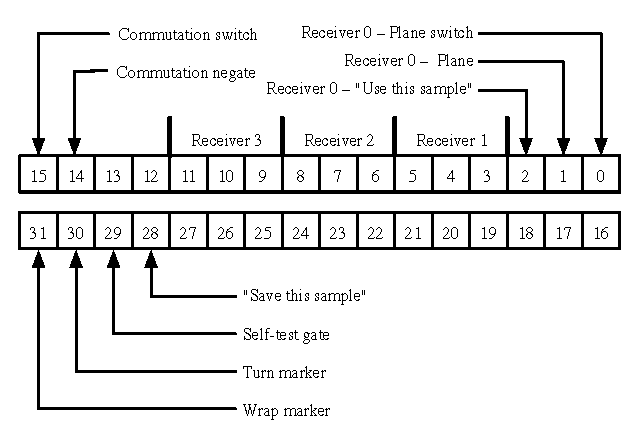
\includegraphics[width=\textwidth]{acquisitionControlRam.eps}
\caption{Acquisition control bit assignments. Courtesy of Eric Norum.}
\label{fig:acquisitionControlRam}
\end{figure}

\item \textbf{examples:}
%

The contents of the file {\tt controlRAM} is converted to control bits
file {\tt RAMcontrolBits}.
\begin{verbatim}
sddsgencontrolbits controlRAM RAMcontrolBits
\end{verbatim}
where the contents of the 3888-row file {\tt controlRAM} are
\begin{verbatim}
2 columns of data:
NAME            UNITS           SYMBOL          FORMAT          TYPE    FIELD  DESCRIPTION
                                                                        LENGTH
Index           NULL            NULL            NULL            long    0       NULL
Waveform        NULL            NULL            NULL            ulong   0       NULL
\end{verbatim}
and the contents of the file {\tt RAMcontrolBits} are mostly short-integer columns
\begin{verbatim}
10 columns of data:
NAME            UNITS           SYMBOL          FORMAT          TYPE    FIELD  DESCRIPTION
                                                                        LENGTH
Index           NULL            NULL            NULL            long    0       NULL
PlaneSwitch     NULL            NULL            NULL            short   0       NULL
Accumulator     NULL            NULL            NULL            short   0       NULL
CommutationNegate NULL            NULL            NULL            short   0       NULL
CommutationSwitch NULL            NULL            NULL            short   0       NULL
Sample          NULL            NULL            NULL            short   0       NULL
TurnMarker      NULL            NULL            NULL            short   0       NULL
WrapMarker      NULL            NULL            NULL            short   0       NULL
SaveSample      NULL            NULL            NULL            short   0       NULL
SelfTest        NULL            NULL            NULL            short   0       NULL
\end{verbatim}
This file {\tt RAMcontrolBits} has two data pages, one page of 3888
rows for the RAM content array, and a second data page of 4096 rows to
simulate what the FPGA transient recorder (i.e. ``scope'') would
record. This data content is the same data as in the first page, but
shifted by 2048 indices, and repeating in both directions to fill 4096
time slots. The second page seems to be superfluous, but it is needed
to produce simulated waveforms in the GUI {\tt MpBPMWaveformViewer}.

Presently the output only return data for one BPM at a time ({\tt
PlaneSwitch},{\tt Accumulator}, and {\tt Sample}) by default the BPM
in position 0 (from receiver positions 0,1,2,3). The column {\tt
Accumulator} is referred to in \cite{Norum2007} as simply ``Plane''.

\item \textbf{synopsis:}
\small
\begin{verbatim}
sddsgencontrolbits <inputRAMFile> <outputFile>
          [-setRAMWaveformPV=<string>] [-controlRAMFile=<filename>] [-comment=<string>] [-receiver=0|1|2|3]
sddsgencontrolbits {-RAMWaveformPV=<string> [-scopeArrayLength=<int>] |
          -scopeWaveformPV=<string> -turnsPerWrap=<int> [-RAMArrayLength=<string>] |
          -RAMWaveformPV=<string> -scopeWaveformPV=<string> } <outputFile>
          [-setRAMWaveformPV=<string>] [-controlRAMFile=<filename>] [-comment=<string>]
sddsgencontrolbits  [-RAMArrayLength=<string>] [-scopeArrayLength=<int>] [-receiver=0|1|2|3]
          {-presetRAMconfiguration=<string>,file=<filename> |
           -planeMode=<string> -commutationMode=<string>]
           -sampleMode={single|continuous|bunchPattern=<string>}
           -bunchPatternFile=<filename> -samplesPerBunch=<int>
           -turnMarkerOffset=<int> -transitionDeadTime=<int> }
           [-scopeTriggerIndexOffset=<int>] [-receiver=0|1|2|3]
           [-setRAMWaveformPV=<string>] [-controlRAMFile=<filename>] [-comment=<string>]
           [-accumulatorMode=<string>] [-turnMarkerInterval=<integer>]
           [-secondSampleBunch=delay=<int>,samplesPerBunch=<int>]
Creates a file of RAM control bits.
Optionally writes to a RAM acquisition control waveform.
Each usage represent one of three ways to supply input data:
1) input file of RAM data,
2) RAM or scope readback waveform PV, or
3) RAM configuration parameters
such as preset bunch pattern and others.
<inputRAMFile>      file containing the values of a RAM waveform record. The data
                    is an array of unsigned long integer.

-RAMWaveformPV      RAM waveform PV name.
-scopeWaveformPV    digital scope waveform PV name.
-RAMArrayLength     the length of control RAM waveform PV needed for generating control bits from
                    bunch pattern.
-scopeArrayLength   the length of digital scope waveform PV needed for generating control bits from
                    bunch pattern.
-turnsPerWrap       number of turns in each wrap;
                    "Simulated" scope readback control bits can normally be generated
                    from RAM long integer data. However for the inverse generation the quantity turnsPerWrap
                    is required. This option is required for the -scopeWaveformPV input method.

-presetRAMconfiguration  specifies a particular configuration from the file of RAM configuration presets.
                    A preset configuration consists of Label, PlaneMode, CommutationMode,
                    SampleMode, BunchPattern, SamplesPerBunch, TurnMarkerOffset, and TransitionDeadTime.
                    The preset string value must match one of the values of Label of the preset file.
                    The default file is /home/helios/oagData/sr/BPMcontrolRAM/presetPatterns.
                    If this option is provided, then the planeMode, commutationMode and sampleMode
                    options will be overridden.
-planeMode          the plane switch mode with values x, y, xy1, or xy2, which stands for
                    x plane, y plane, switch x/y per turn, or switch x/y every two turns.
                    (each turn has 324 time slots.)
-commutationMode    commutation switch mode with possible values of a, b, ab1, and ab2,
                    which stands for 0 degree, 180 degrees, switch between 0 and 180 every turn,
                    or switch  between 0 and 180 every two turns.
-sampleMode         sample mode with values continuous, single or pattern.
                    If "pattern" is selected, then the value of suboption bunchPattern must be given
                    and must match up with a bunch pattern defined in the preset bunch pattern file.
-bunchPatternFile   file that contains the properties of preset bunch patterns.
-accumulatorMode    accumulation switch mode; defaults to the plane mode if omitted.
-transitionDeadTime dead time length in units of timing slots for which samples will not be taken.
-turnMarkerOffset   the offset of turn marker. The first turn marker starts from this offset, and
                    the others are spaced 324 time steps.
-samplesPerBunch    number of consectuive samples to be collected per bunch. Presently it
                    is the same for all bunches.
-turnMarkerInterval turn marker interval, default is 324.
-secondSampleBunch  add a second sample bunch; delay gives the offset from the first bunch
                    and samplesPerBunch sets the number of samples.
-scopeTriggerIndexOffset  provides the offset between scope trigger and wrap marker
                    (which is normally set at 2048 by PV S42B:scope:gtr:numberPTS).

The output options are the same in the three usages.
<outputFile>        file of the separated control bits of a RAM waveform record.
                    Columns are Index, PlaneSwitch, CommutationSwitch, Sample,
                    TurnMarker, P0Marker, WrapMarker, all short integers except for Index,
                    which is long integer.
                    The digital scope readback waveform record is simulated and is
                    included as the second data page.
-setRAMWaveformPV   if provided, the control RAM long integer data will be written to this PV.
                    Note that when used with -RAMWaveformPV input with the same PVs,
                    the same values are read and written to the same PV.
-controlRAMFile     if provided, the control RAM long integer data will be written to this file.
-comment            provide comments for saving the control RAM into controlRAMFile .
-receiver           provide the receiver number to select from the control RAM when
                    creating the control bits file, which has room for only one set
                    of flags. When setting RAM all receivers have the same flags.
Program by H. Shang, ANL (EPICS 3.14.8.2, Mar 26 2007).

\end{verbatim}
\normalsize

\item \textbf{files:}
\begin{itemize}
  \item \textbf{input file:} \par
  RAM waveform record containing unsigned long integer values.
  \item \textbf{output file:} \par
  Control bits separated into individual columns; includes simulated scope readback page.
  \item \textbf{bunch pattern file:} \par
  Definitions of preset bunch patterns for pattern-based sampling modes.

  \item \textbf{switches:}
  \begin{itemize}
    \item {\tt -RAMWaveformPV} --- RAM waveform PV name.
    \item {\tt -scopeWaveformPV} --- digital scope waveform PV name.
    \item {\tt -planeMode} --- plane switch mode for receivers.
    \item {\tt -accumulatorMode} --- accumulation switch mode.
    \item {\tt -commutationMode} --- commutation switch mode.
    \item {\tt -sampleMode} --- sampling mode, including bunch patterns.
    \item {\tt -bunchPatternFile} --- file of preset bunch patterns.
    \item {\tt -samplesPerBunch} --- samples collected per bunch.
    \item {\tt -secondSampleBunch} --- add delayed second sample bunch.
    \item {\tt -turnMarkerOffset} --- offset to first turn marker.
    \item {\tt -turnMarkerInterval} --- interval between turn markers.
    \item {\tt -transitionDeadTime} --- dead time in timing slots.
    \item {\tt -RAMArrayLength} --- length of control RAM waveform PV.
    \item {\tt -scopeArrayLength} --- length of scope waveform PV.
    \item {\tt -turnsPerWrap} --- number of turns per wrap for scope data.
    \item {\tt -scopeTriggerIndexOffset} --- offset between scope trigger and wrap marker.
    \item {\tt -setRAMWaveformPV} --- write control RAM data to this PV.
    \item {\tt -controlRAMFile} --- write control RAM data to this file.
    \item {\tt -comment} --- comment string saved with control RAM data.
    \item {\tt -receiver} --- select receiver when creating control bits (obsolete).
  \end{itemize}
\end{itemize}

\item \textbf{see also:}
\begin{itemize}
% replacing <prog> with the program to be referenced:
  \item \progref{sddsexperiment}
\end{itemize}
\item \textbf{author:} L. Emery, H. Shang, R. Soliday, ANL
\end{sddsprog}

%
% Template for making SDDS Toolkit manual entries.
%
\begin{sddsprog}{sddsglitchlogger}
\item {\bf description:}
%
% Insert text of description (typically a paragraph) here.
%
\verb+sddsglitchlogger+ reads values of process variables and writes them to a file at a specified time interval when a trigger occurs.
An input file defines the process variables to be monitored and/or the trigger parameters.
An trigger file defines the the process variables that act as triggers.
\item {\bf example:} 
%
% Insert text of examples in this section.  Examples should be simple and
% should be proceeded by a brief description.  Wrap the commands for each
% example in the following construct:
% 
%
The position readbacks of PMs in linac are monitored with the command below.
\begin{verbatim}
sddsglitchlogger SRvac.mon . -time=24,hours -sampleInterval=1,minute
\end{verbatim}
``.'' specifies the directory of the outputfile is current directory,the file name is generated
as related to the date.
where the contents of the file \verb+SRvac.mon+ are
\begin{verbatim}
SDDS1
&parameter name=TriggerControlName type=string &end
&parameter name=MajorAlarm type=short &end
&parameter name=MinorAlarm, type=short &end
&parameter name=NoAlarm type=short &end
&parameter name=OutputRootname type=string &end
&column name=ControlName type=string  &end
&column name=ReadbackName type=string &end
&column name=ReadbackUnits type=string &end
&data mode=ascii no_row_counts=1 &end
!page 1
soliday:PM1:X:positionM
0
0
1
PM
soliday:PM1:X:positionM  soliday:PM1:X:positionM  mm
soliday:PM1:Y:positionM  soliday:PM1:Y:positionM  mm
soliday:PM2:X:positionM  soliday:PM2:X:positionM  mm
...
\end{verbatim}
\item {\bf synopsis:} 
%
% Insert usage message here:
%
\begin{verbatim}
usage: sddsglitchlogger <input> <outputDirectory>|<outputRootname> [-triggerFile=<filename>]
        [-lockFile=<filename>[,verbose]] [-sampleInterval=<secs>] [-time=<real-value>[,<time-units>]
        [-circularBuffer=[before=<number>,][after=<number>]] [-delay=<steps>]
        [-holdoffTime=<seconds>] [-autoHoldoff] [-pendIOtime=<value>]
        [-inhibitPV=name=<name>[,pendIOTime=<seconds>][,waitTime=<seconds>]]
        [-conditions=<filename>,{allMustPass | oneMustPass}]
        [-verbose] [-watchInput]
        [-runControlPV=string=<string>,pingTimeout=<value>]
        [-runControlDescription=string=<string>]
Writes values of process variables or devices to a binary SDDS file.
\end{verbatim}
\item {\bf files:}
% Describe the files that are used and produced
\begin{itemize}
\item {\bf input file:}\par
The input file is an SDDS file with a few data columns required:
\begin{itemize}
        \item {\tt ControlName} or {\tt Device} --- Required string column for the names of the process variables
                or devices to be monitored. Both column names are equivalent.
        \item {\tt ReadbackName} --- Optional string column for the names of the data columns in the 
                output file. If absent, process variable or device name is used.
        \item {\tt ReadbackUnits} --- Optional string column for the units fields of the data columns in the 
                output file.If absent, units are null.
\end{itemize}
If triggerFile that gives the trigger information is not given, the input file should contain following
parameters:
\begin{itemize}
        \item {\tt OutputRootname} --- Required string parameter for the root name of output file.
                Different OutputRootmames go to different output files. If different pages have the same 
                OutputRootname, the columns defined in new pages are ignored. Only the trigger defined in
                newer page is counted to the same output.
        \item {\tt TriggerControlName} --- Required string parameter for the name of process variable that
                acts as trigger.
        \item {\tt MajorAlarm}  --- Optional short parameter for alarm-based trigger.
                if nonzero, then severity of MAJOR on TriggerControlName, results in a buffer dump.
        \item {\tt MinorAlarm}  --- Optional short parameter for alarm-based trigger.
                if nonzero, then severity of MINOR on TriggerControlName, results in a buffer dump.
        \item {\tt NoAlarm}  --- Optional short parameter for alarm-based trigger.
                if nonzero, then severity of NOALARM on TriggerControlName, results in a buffer dump.
        \item {\tt TransitionDirection}  --- Optional short parameter for transition-based trigger.
                required if TransitionThreshold parameter is defined.
\begin{itemize}
        \item {\tt -1}  transition of TriggerControlName from above threshold to below threshold.
                        results in buffer dump.
        \item {\tt 0}   ignore transition-based triggers for this PV.
        \item {\tt 1}   transition from below threshold to above threshold results in buffer dump.
\end{itemize}
        \item {\tt TransitionThreshold}  --- Optional double parameter for transition-based trigger.
                required if TransitionDirection parameter is defined. It defines the threshold of
                a transition trigger.
        \item {\tt GlitchThreshold} --- Optional double parameter for glitch-based trigger.
\begin{itemize}
        \item {\tt 0}   ignore glitch-based triggers for this PV.
        \item {\tt >0}   absolute glitch level.
        \item {\tt <0}   -1*(fractional glitch level).
\end{itemize}
        \item {\tt GlitchBaselineSamples} --- Optional long parameter for glitch-based trigger.
                It defines number of samples to average to get the baseline value for glitch determination.
                A glitch occurs when newReading is different from the baseline by more than GlitchThreshold
                or (if GlitchThreshold<0) by |GlitchThreshold*baseline|.
        \item {\tt GlitchBaselineAutoReset} --- Optional short parameter for glitch-based trigger.
                Normally (if there is no glitch) the baseline is updated at each step using
                baseline -> (baseline*samples+newReading)/(samples+1).  After a glitch, one 
                may want to do something different. 
 \begin{itemize}       
        \item {\tt 1}   After a glitch, the baseline is reassigned to its current value.
        \item {\tt 0}   The pre-glitch baseline is retained. 
\end{itemize}
\end{itemize}
\item {\bf trigger file:}\par
The trigger file is an SDDS file with following columns, the meaning of these columns are the same as
the parameters defined in input file, which are replaced by a trigger file:
\begin{itemize}
        \item {\tt TriggerControlName} --- Required string column for the names of the process variables
                that act as triggers.
        \item {\tt MajorAlarm} --- Optional short column.
        \item {\tt MinorAlarm} --- Optional short column.
        \item {\tt NoAlarm} --- Optional short column.
        \item {\tt TransitionThreshold} --- Optional double column. (required for transition trigger exists)
        \item {\tt TransitionDirection} --- Optional short column.(required for transition trigger exists)
        \item {\tt GlitchThreshold} --- Optional double column.(required for glitch trigger exists)
        \item {\tt GlitchBaselineSamples} --- Optional long column.
        \item {\tt GlitchBaselineAutoReset} --- Optional short column
\end{itemize}
\item {\bf conditions file:} \par
The conditions file is an optional input file specified on the command line which lists
conditions that must be satisfied at each time step before the data can be logged.

The file is like the main input file, but has numerical columns \verb+LowerLimit+ and \verb+UpperLimit+.
The minimal column set is \verb+ControlName+, which contain the PV names, and the two limits columns above.
Depending on command line options, when any or all PV readback from this file
is outstide the range defined by the corresponding data from \verb+LowerLimit+ and \verb+UpperLimit+,
none of the data of the input file PVs are recorded. 
When this situation occurs for a long period of time, the size of the output file doesn't
grow, and it may appear that the monitoring process has somehow stopped.
It is possible to check the program activity with the \verb+touch+ sub-option
which causes the monitoring program to touch the output file at every step.

\item {\bf output file:}\par
If trigger file is not given, the output file name is:
   outputDirectory/OutputRootname-string
   here, there may be many output files depends how many pages and how many different OutputRootnames 
   the input file has.
If trigger file is given, the outputDirectory given in command line is actually the OutputRootname,
the output file name is now (only one output in this case):
   outputDirectory-string
In above, both string is generated by MakeDailyGenerationFilename().

The output file contains one data column for each process variables named in the input file. 
Time columns and other miscellaneous columns are defined: 
\begin{itemize}
        \item {\tt Time} --- Double column of time since start of epoch. This time data can be used by
        the plotting program {\verb+sddsplot+} to make the best choice of time unit conversions
        for time axis labeling.
        \item {\tt TimeOfDay} --- Float column of system time in units of hours. 
        The time does not wrap around at 24 hours.
        \item {\tt DayOfMonth} --- Float column of system time in units of days. 
        The day does not wrap around at the month boundary.
        \item {\tt Step} --- Long column for step number.
        \item {\tt CAerrors} --- Long column for number of channel access errors at each reading step. 
\end{itemize}

Many time-related parameters are defined in the output file:
\begin{itemize}
        \item {\tt TimeStamp} --- String parameter for time stamp for file.
        \item {\tt PageTimeStamp} --- String parameter for time stamp for each page. When data
                is appended to an existing file, the new data is written to a new
                page. The {\tt PageTimeStamp} value for the new page is the creation
                date of the new page. The {\tt TimeStamp} value for the new page is the creation 
                date of the very first page.
        \item {\tt StartTime} --- Double parameter for start time from the {\tt C} time call cast to type double.
        \item {\tt YearStartTime} --- Double parameter for start time of present year from the {\tt C} time call cast to type double.
        \item {\verb+StartYear+} --- Short parameter for the year when the file was started.
        \item {\verb+StartJulianDay+} --- Short parameter for the day when the file was started.
        \item {\verb+StartMonth+} --- Short parameter for the month when the file was started.
        \item {\verb+StartDayOfMonth+} --- Short parameter for the day of month when the file was started.
        \item {\verb+StartHour+} --- Short parameter for the hour when the file was started.
\end{itemize}
\end{itemize}

%
\item {\bf switches:}
%
% Describe the switches that are available
%
    \begin{itemize}

        \item {\tt -triggerFile} --- specifies the name of trigger file.
        \item {\tt -lockFile} --- specifies the name of lock file. When this option is given,
                sddsglitchlogger uses the named file to prevent running multiple versions of
                the program.  If the named file exists and is locked, the program exits.  
                If it does not exist or is not locked, it is created and locked.
        \item {\tt -sampleInterval=<real-value>[,<time-units>]} --- Specifies the interval between readings.
                The time interval is implemented with a call to usleep between calls to the control system.
                Because the calls to the control system may take up a significant amount of time, the average
                effective time interval may be longer than specified.
        \item {\tt -time=<real-value>[,<time-units>]} --- Total time for monitoring. Valid time units are
                seconds, minutes, hours, and days. The completion time may be longer, because the time
                interval in not guaranteed.
        \item {\tt -circularBuffer} --- Set how many samples to keep before and after the triggering event.
        \item {\tt -delay=<steps>} --- Used to delay reading PVs after a glitch or trigger. Useful when
                waveform PVs act as a circular buffer.
        \item {\tt -holdoffTime} --- Set the number of seconds to wait after a trigger or alarm before
                accepting new triggers or alarms.
        \item {\tt -autoHoldoff} --- Sets holdoff time so that the after-trigger samples are guaranteed
                to be collected before a new trigger or alarm is accepted.
        \item {\tt -verbose} --- Prints out a message when data is taken.
        \item {\tt -pendIOtime=<value>} --- sets the maximum time to wait for return of each value.
        \item {\tt -inhibitPV} --- Checks this PV prior to each sample.  If the value is nonzero,
                then data collection is inhibited.  None of the conditions-related or other PVs are polled.
        \item {\tt -watchInput} --- If it is given, then the programs checks the input file to see if
                it is modified. If the inputfile is modified, then read the input files again and start
                the logging.
        \item {\tt -runControlPV=string=<string>,pingTimeout=<value>} --- specifies a runControl PV name
                and ping timeout.
        \item {\tt -runControlDescription=string=<string>} --- specifies a runControl PV description record.
        \item {\verb+-conditions=<filename>,{allMustPass | oneMustPass}[,touchOutput][,retakeStep]+} ---
                   Names an SDDS file containing PVs to read and limits on each PV that must
                   be satisfied for data to be taken and logged.  The file is like the main
                   input file, but has numerical columns LowerLimit and UpperLimit.

                One of \verb+allMustPass+ or \verb+oneMustPass+ must be specified. It would make sense
                to use \verb+allMustPass+ in most monitoring applications.
                If \verb+touchOutput+ is present, then the output file is touched, even if no data
                is written. This way, one can determine by the time stamp of the file
                whether the monitoring job is still alive
                when the conditions fail for a long period of time. If \verb+retakeStep+ is
                present, then the value of \verb+Step+ in the output file is not
                incremented until the conditions pass, and data is written to the output file.
    \end{itemize}

\item {\bf see also:}
    \begin{itemize}
%
% Insert references to other programs by duplicating this line and 
% replacing <prog> with the program to be referenced:
%
    \item \progref{sddsmonitor}
    \end{itemize}
%
% Insert your name and affiliation after the '}'
%
\item {\bf author: Hairong Shang, ANL} 
\end{sddsprog}

%
% Template for making SDDS Toolkit manual entries.
%
\begin{sddsprog}{sddsimagemonitor}
\item {\bf description:}
\verb+sddsimagemonitor+ reads EPICS image process variables and writes the image
  data to an SDDS file at regular intervals. Image PVs may be supplied from an
  input file or directly on the command line. Optional scalar PVs can be logged as
  parameters, and data may be conditioned on other PV values. Two-dimensional
  images produce one page per acquisition, while multi-plane data result in one
  page per plane.
\item {\bf example:}
The following command logs a set of camera images once per minute.
\begin{verbatim}
sddsimagemonitor cam.mon cam.sdds -interval=1,minute -steps=10
\end{verbatim}
where the contents of the file \verb+cam.mon+ are
\begin{verbatim}
SDDS1
&column name=WaveformPV, type=string &end
&data mode=ascii no_row_counts=1 &end
AR:SLM1:image1
\end{verbatim}
\item {\bf synopsis:}
\begin{verbatim}
usage: sddsimagemonitor [<inputfile> | -PVnames=<name>[,<name>]] <outputfile>
    [{-erase | -generations[=digits=<integer>][,delimiter=<string>]} [-pendIOtime=<seconds>]
    [-steps=<integer> | -time=<value>[,<units>]] [-interval=<value>[,<units>]]
    [-enforceTimeLimit] [-offsetTimeOfDay]
    [-verbose] [-singleShot{=noprompt|stdout}] [-precision={single|double}]
    [-dataType={short|long|float|double|character|string}]
    [-onCAerror={useZero|skipPage|exit}]
    [-scalars=<filename>] [-flushSteps=<integer>]
    [-conditions=<filename>,{allMustPass|oneMustPass}[,touchOutput][,retakeStep]]
    [-comment=<parameterName>,<text>] [-nowarnings]
    [-xParameter=dimension=<value>[,name=<name>][,minimum=<value>][,maximum=<value>][,interval=<value>]]
    [-yParameter=dimension=<value>[,name=<name>][,minimum=<value>][,maximum=<value>][,interval=<value>]]
    [-singleColumn] [-logOnChange] [-device=<name>] [-retakeStep]
\end{verbatim}
\item {\bf switches:}
  \begin{itemize}
  \item {\verb+-PVnames=<name>[,<name>]+} --- specifies image PV names to read.
  \item {\verb+-scalars=<filename>+} --- logs scalar PVs as parameters in the output file.
  \item {\tt -erase} --- overwrites the output file if it exists.
  \item {\verb+-generations[=digits=<integer>][,delimiter=<string>]+} --- writes to a unique generation file.
  \item {\verb+-pendIOtime=<seconds>+} --- sets the wait time for channel access searches.
  \item {\verb+-steps=<integer>+} --- number of image acquisitions to perform.
  \item {\verb+-time=<value>[,<units>]+} --- total acquisition time; seconds, minutes, hours, or days.
  \item {\verb+-interval=<value>[,<units>]+} --- desired time between acquisitions.
  \item {\tt -enforceTimeLimit} --- enforces the time limit given with \verb+-time+.
  \item {\tt -offsetTimeOfDay} --- adjusts the starting \verb+TimeOfDay+ value.
  \item {\tt -verbose} --- prints a message when data are taken.
  \item {\verb+-singleShot[=noprompt|stdout]+} --- single acquisition triggered by a key press.
  \item {\verb+-precision={single|double}+} --- sets data precision for image PVs.
  \item {\verb+-dataType={short|long|float|double|character|string}+} --- forces an SDDS data type.
  \item {\verb+-onCAerror={useZero|skipPage|exit}+} --- action to take on channel access errors.
  \item {\verb+-flushSteps=<integer>+} --- buffers this many steps before writing to the file.
  \item {\verb+-conditions=<filename>,{allMustPass|oneMustPass}[,touchOutput][,retakeStep]+} ---
        applies limits from a conditions file to gate data logging.
  \item {\verb+-comment=<parameterName>,<text>+} --- inserts a comment parameter with the given text.
  \item {\tt -nowarnings} --- suppresses warning messages.
  \item {\verb+-xParameter=dimension=<value>[,name=<name>][,minimum=<value>][,maximum=<value>][,interval=<value>]+} ---
        defines X-axis parameter information.
  \item {\verb+-yParameter=dimension=<value>[,name=<name>][,minimum=<value>][,maximum=<value>][,interval=<value>]+} ---
        defines Y-axis parameter information.
  \item {\tt -singleColumn} --- writes image data to a single column with index parameters.
  \item {\tt -logOnChange} --- writes data only if scalar PVs change.
  \item {\verb+-device=<name>+} --- selects the device type (e.g., areadector or FLID).
  \item {\tt -retakeStep} --- repeats a step if timestamps or scalar values do not change.
  \end{itemize}
\item {\bf see also:}
  \begin{itemize}
  \item \progref{sddsmonitor}
  \item \progref{sddsvmonitor}
  \item \progref{sddswmonitor}
  \end{itemize}
\item {\bf author:} M. Borland, L. Emery, H. Shang, R. Soliday, ANL
\end{sddsprog}

% sddslogger: log PV values at intervals defined in an input file.
\begin{sddsprog}{sddslogger}
\item \textbf{description:}
\verb+sddslogger+ reads values of process variables and writes them to a file at a specified time interval.
One or more input files defines the process variables to be monitored.
\item \textbf{examples:}
The pressure readbacks of storage ring ion pumps and the stored current are monitored
with the command below.
\begin{verbatim}
sddslogger SRvac.mon SRvac.sdds -time=24,hours -sampleInterval=1,minutes
\end{verbatim}
where the contents of the file \verb+SRvac.mon+ are
\begin{verbatim}
SDDS1
&description &end
&column
 name = ControlName,  type = string, &end
&column
 name = ControlType,  type = string, &end
&column
 name = ReadbackUnits,  type = string, &end
&column
 name = ReadbackName,  type = string, &end
&data
 mode = ascii, no_row_counts=1 &end
! page number 1
S35DCCT:currentCC pv mA S35DCCT
VM:01:3IP1.VAL pv Torr VM:01:3IP1
VM:01:2IP2.VAL pv Torr VM:01:2IP2
VM:01:2IP3.VAL pv Torr VM:01:2IP3
...
\end{verbatim}
\item \textbf{synopsis:}
\begin{verbatim}
usage: sddslogger <SDDSinputfile1> <SDDSoutputfile1> <SDDSinputfile2> <SDDSoutputfile2>...
    [-generations[=digits=<integer>][,delimiter=<string>][,rowlimit=<number>][,timelimit=<secs>] | -dailyFiles | -monthlyFiles]
    [-sampleInterval=<real-value>[,<time-units>]]
    [-logInterval=<integer-value>] [-flushInterval=<integer-value>]
    [-steps=<integer-value> | -time=<real-value>[,<time-units>]]
    [-enforceTimeLimit] [-offsetTimeOfDay]
    [-verbose] [-singleshot{=noprompt | stdout}]
    [-precision={single|double}]
    -onerror={usezero|skiprow|exit} [-pendIOtime=<value>]
    [-conditions=<filename>,{allMustPass | oneMustPass}[,touchOutput][,retakeStep]]
Writes values of process variables or devices to a binary SDDS file.
\end{verbatim}
\item \textbf{files:}
\begin{itemize}
  \item \textbf{input file(s):}\par
      The input files are SDDS files with a few data columns required:
  \begin{itemize}
    \item {\tt ControlName} or {\tt Device} --- Required string column for the names of the process variables
          or devices to be monitored. Both column names are equivalent.
    \item {\tt ReadbackUnits} --- Required string column for the units fields of the data columns in the
          output file.
    \item {\tt ReadbackName} --- Optional string column for the names of the data columns in the
          output file. If absent, process variable or device name is used.
    \item {\tt Message} --- Optional string column for the device read message. If a row entry in
          column {\tt ControlName} is a process variable, then the corresponding entry
          in {\tt Message} should be a null string.
    \item {\tt ScaleFactor} --- Optional double column for a factor with which to multiply
          values of the readback in the output file.
    \item {\tt Average} --- Optional long column.  If value is non-zero the process variable will have
          its average value logged.  Otherwise it will log the most recent value.
          values of the readback in the output file.
    \item {\tt DoublePrecision} --- Optional long column. If value is non-zero the process variable
          will be logged as a double-precision number.  Otherwise it will be logged as a single-precision
          number.
  \end{itemize}

  \item \textbf{conditions file:} \par
      The conditions file is an optional input file specified on the command line which lists
      conditions that must be satisfied at each time step before the data can be logged.

      The file is like the main input file, but has numerical columns \verb+LowerLimit+ and \verb+UpperLimit+.
      The minimal column set is \verb+ControlName+, which contain the PV names, and the two limits columns above.
      Depending on command line options, when any or all PV readback from this file
      is outstide the range defined by the corresponding data from \verb+LowerLimit+ and \verb+UpperLimit+,
      none of the data of the PVs in the input files are recorded.
      When this situation occurs for a long period of time, the size of the output files doesn't
      change, and it may appear that the monitoring process has somehow stopped.
      It is possible to check the program activity with the \verb+touch+ sub-option
      which causes the logging program to touch the output file at every step.

  \item \textbf{output file(s):}\par
      The output files contains one data column for each process variable named in the corresponding input file. By default,
      the data type is float (single precision).
      Time columns and other miscellaneous columns are defined:
  \begin{itemize}
    \item {\tt Time} --- Double column of time since start of epoch. This time data can be used by
          the plotting program {\verb+sddsplot+} to make the best choice of time unit conversions
          for time axis labeling.
    \item {\tt TimeOfDay} --- Float column of system time in units of hours.
          The time does not wrap around at 24 hours.
    \item {\tt DayOfMonth} --- Float column of system time in units of days.
          The day does not wrap around at the month boundary.
    \item {\tt Step} --- Long column for step number.
    \item {\tt CAerrors} --- Long column for number of channel access errors at each reading step.
  \end{itemize}

      Many time-related parameters are defined in the output file:
  \begin{itemize}
    \item {\tt TimeStamp} --- String parameter for time stamp for file.
    \item {\tt PageTimeStamp} --- String parameter for time stamp for each page. When data
          is appended to an existing file, the new data is written to a new
          page. The {\tt PageTimeStamp} value for the new page is the creation
          date of the new page. The {\tt TimeStamp} value for the new page is the creation
          date of the very first page.
    \item {\tt StartTime} --- Double parameter for start time from the {\tt C} time call cast to type double.
    \item {\tt YearStartTime} --- Double parameter for start time of present year from the {\tt C} time call cast to type double.
    \item {\verb+StartYear+} --- Short parameter for the year when the file was started.
    \item {\verb+StartJulianDay+} --- Short parameter for the day when the file was started.
    \item {\verb+StartMonth+} --- Short parameter for the month when the file was started.
    \item {\verb+StartDayOfMonth+} --- Short parameter for the day of month when the file was started.
    \item {\verb+StartHour+} --- Short parameter for the hour when the file was started.
  \end{itemize}
\end{itemize}

\item \textbf{switches:}
\begin{itemize}
%   \item {\tt -pipe[=input][,output]} --- The standard SDDS Toolkit pipe option.
  \item {\verb+-generations[=digits=<integer>][,delimiter=<string>]+} ---
      The output is sent to the file \verb+<SDDSoutputfile>-<N>+, where \verb+<N>+ is
      the smallest positive integer such that the file does not already
      exist.  By default, four digits are used for formatting \verb+<N>+, so that
      the first generation number is 0001.
  \item {\tt -dailyFiles} --- Starts a new output file each day. Optional qualifiers
      \verb+rowlimit+, \verb+timelimit+, \verb+timetage+, and \verb+verbose+ control
      file rollover behavior.
  \item {\tt -monthlyFiles} --- Starts a new output file each month with the same optional
      qualifiers as \verb+-dailyFiles+.
  \item {\tt -sampleInterval=<real-value>[,<time-units>]} --- Specifies the interval between readings. The time
      interval is implemented with a call to usleep between calls to the control system.
      Because the calls to the control system may take up a significant amount of time, the average
      effective time interval may be longer than specified.
  \item {\tt -logInterval=<interval>} --- Specifies the number of sampling intervals to average before
      writing to the output file.
  \item {\tt -flushInterval=<interval>} --- Number of sampling intervals between forced flushes of data to disk.
  \item {\tt -steps=<integer-value>} --- Number of readbacks for each process variable before normal exiting.
  \item {\tt -time=<real-value>[,<time-units>]} --- Total time for monitoring. Valid time units are
      seconds, minutes, hours, and days. The program calculates the number of steps by dividing this time
      by the interval. The completion time may be longer, because the time interval in not guaranteed.
  \item {\tt -enforceTimeLimit} --- Enforces the time limit given even if the expected number of samples has
      not been taken.
  \item {\tt -offsetTimeOfDay} --- Adjusts the starting TimeOfDay value so that it corresponds to the
      day for which the bulk of the data is taken.  Hence, a 26 hour job started at 11pm would have an
      initial time of day of -1 hour and a final time of day of 25 hours.
  \item {\tt -verbose} --- Prints out a message when data is taken.
  \item {\verb+-singleshot[=noprompt]+} --- a single read is prompted at the terminal
      and initiated by a \verb+<cr>+ key press. The time interval is disabled.
      With \verb+noprompt+ present, no prompt is written to the terminal, but a \verb+<cr>+
      is still expected. Typing ``q'' or ``Q'' terminates the monitoring.
  \item {\tt -precision={single|double}} --- Sets floating-point precision for logged data.
  \item {\tt -onerror=\{usezero|skiprow|exit\}} --- Selects action taken when a channel access error occurs.
      The default is using zero ({\tt usezero}) for the value of the process variable
      with the channel access error, and resuming execution. The second option ({\tt skiprow}) is to
      simply throw away all the data for that read step, and resume execution.
      the third option is to exit the program.
  \item {\tt -pendIOtime=<value>} --- Sets the maximum time to wait for connection to each PV.
  \item {\verb+-conditions=<filename>,{allMustPass | oneMustPass}[,touchOutput][,retakeStep]+} ---
      Names an SDDS file containing PVs to read and limits on each PV that must
      be satisfied for data to be taken and logged.  The file is like the main
      input file, but has numerical columns LowerLimit and UpperLimit.

      One of \verb+allMustPass+ or \verb+oneMustPass+ must be specified. It would make sense
      to use \verb+allMustPass+ in most monitoring applications.
      If \verb+touchOutput+ is present, then the output file is touched, even if no data
      is written. This way, one can determine by the time stamp of the file
      whether the monitoring job is still alive
      when the conditions fail for a long period of time. If \verb+retakeStep+ is
      present, then the value of \verb+Step+ in the output file is not
      incremented until the conditions pass, and data is written to the output file.
\end{itemize}

\item \textbf{see also:}
\begin{itemize}
  \item \progref{sddsmonitor}
  \item \progref{sddsvmonitor}
  \item \progref{sddswmonitor}
  \item \progref{sddssnapshot}
\end{itemize}
\item \textbf{author:} R. Soliday, M. Borland, H. Shang ANL
\end{sddsprog}

% sddslogonchange: log PV values only when they change.
\begin{sddsprog}{sddslogonchange}
\item \textbf{description:}
\verb+sddslogonchange+ records only the values of process variables that change. This reduces the output file size if process variables do not change often.
\item \textbf{examples:}
Process variable setpoints from the storage ring are monitored
with the command below.
\begin{verbatim}
sddslogonchange SR.loc SR.sdds -logInitialValues -watchInput -connectTimeout=120
\end{verbatim}
where the contents of the file \verb+SR.loc+ are
\begin{verbatim}
SDDS1
&column name=ControlName, type=string,  &end
&column name=Tolerance, format_string=%g, type=double,  &end
&column name=Description, type=string,  &end
&data mode = ascii, no_row_counts=1 &end
! page number 1
S1A:H1:CurrentAI.AOFF 0.0 ""
S1A:H2:CurrentAI.AOFF 0.0 ""
S1A:H3:CurrentAI.AOFF 0.0 ""
...
\end{verbatim}
\item \textbf{synopsis:}
\begin{verbatim}
usage: sddslogonchange <input> <output>
  [-timeDuration=<realValue>[,<time-units>]]
  [-append[=recover]]
  [-eraseFile]
  [-generations[=digits=<integer>][,delimiter=<string>]]
  [-dailyFiles]
  [-pendEventTime=<seconds>]
  [-durations]
  [-connectTimeout=<seconds>]
  [-explicit[=only]]
  [-verbose]
  [-comment=<parameterName>,<text>]
  [-requireChange[=severity][,status][,both]]
  [-inhibitPV=name=<name>[,pendIOTime=<seconds>][,waitTime=<seconds>]]
  [-includeTimeOfDay]
  [-offsetTimeOfDay]
  [-logInitialValues]
  [-logAlarms]
  [-watchInput]
  [-runControlPV=string=<string>,pingTimeout=<value>]
  [-runControlDescription=string=<string>]
  [-sddslogger]
  [-noToleranceMinLimit]

Logs data for the process variables named in the ControlName
column of <input> to an SDDS file <output>.
\end{verbatim}
\item \textbf{files:}
\begin{itemize}
  \item \textbf{input file:}\par
The input file is an SDDS file with only one data column required:
  \begin{itemize}
    \item {\tt ControlName} --- Required string column for the names of the process variables or devices to be monitored.
    \item {\tt ReadbackName} --- Optional string column.
    \item {\tt ReadbackUnits} --- Optional string column.
    \item {\tt Description} --- Optional string column.
    \item {\tt RelatedControlName} --- Optional string column.
    \item {\tt Tolerance} --- Optional numeric column which contains a tolerance value to avoid logging small changes.
  \end{itemize}

  \item \textbf{output file:}\par
The output file contains parameters, arrays, and columns.
  \begin{itemize}
    \item {\bf Parameters}
    \item {\tt InputFile} --- sddslogonchange input file.
    \item {\tt TimeStamp} --- Time stamp for file.
    \item {\tt PageTimeStamp} --- Time stamp for page.
    \item {\tt StartTime} --- Start time.
    \item {\tt YearStartTime}
    \item {\tt StartYear}
    \item {\tt StartJulianDay}
    \item {\tt StartMonth}
    \item {\tt StartDayOfMonth}
    \item {\tt StartHour}
  \end{itemize}
\begin{verbatim}

\end{verbatim}
  \begin{itemize}
    \item {\bf Arrays}
    \item {\tt ControlName} --- Control names of process variables
    \item {\tt ReadbackName} --- Optional readback names of process variables
    \item {\tt ReadbackUnits} --- Optional units of process variables
    \item {\tt AlarmStatusString} --- Optional
    \item {\tt AlarmSeverityString} --- Optional
    \item {\tt DescriptionString} --- Optional
    \item {\tt RelatedControlName} --- Optional
  \end{itemize}
\begin{verbatim}

\end{verbatim}
  \begin{itemize}
    \item {\bf Columns}
    \item {\tt ControlNameIndex} --- Index of the ControlName array.
    \item {\tt Value} --- Value of the process variable.
    \item {\tt Time} --- Time stamp of the change in value.
    \item {\tt PreviousRow} --- Previous row with an identical ControlNameIndex value.
    \item {\tt AlarmStatusIndex} --- Optional
    \item {\tt AlarmSeverityIndex} --- Optional
    \item {\tt Duration} --- Optional
    \item {\tt RelatedValueString} --- Optional
    \item {\tt ControlName} --- Optional
    \item {\tt AlarmStatus} --- Optional
    \item {\tt AlarmSeverity} --- Optional
    \item {\tt Description} --- Optional
    \item {\tt RelatedControlName} --- Optional

  \end{itemize}

\end{itemize}

\item \textbf{switches:}
\begin{itemize}
%   \item {\tt -pipe[=input][,output]} --- The standard SDDS Toolkit pipe option.
  \item {\tt -timeDuration=<realValue>[,<time-units>]} --- Specifies time duration for logging.  The default time units are seconds; you may also specify days, hours, or minutes.
  \item {\tt -offsetTimeOfDay} --- Adjusts the starting TimeOfDay value so that it corresponds to the day for which the bulk of the data is taken.  Hence, a 26 hour job started at 11pm would have initial time of day of -1 hour and final time of day of 25 hours.
  \item {\tt -append[=recover]} --- Specifies appending to the file <output> if it exists already. If the recover qualifier is given, recovery of a corrupted file is attempted using sddsconvert, at the risk of loss of some of the data already in the file.
  \item {\tt -eraseFile} --- Specifies erasing the file <output> if it exists already.
  \item {\tt -generations[=digits=<integer>][,delimiter=<string>]} --- Specifies use of file generations.  The output is sent to the file <output>-<N>, where <N> is the smallest positive integer such that the file does not already exist.   By default, four digits are used for formatting <N>, so that the first generation number is 0001.
  \item {\tt -dailyFiles} --- The output is sent to the file <output>-YYYY-JJJ-MMDD.<N>, where YYYY=year, JJJ=Julian day, and MMDD=month+day.  A new file is started after midnight.
  \item {\tt -pendEventTime=<seconds>} --- Specifies the CA pend event time, in seconds.  The default is 10.
  \item {\tt -durations} --- Specifies including state duration and previous row reference data in output.
  \item {\tt -connectTimeout=<seconds>} --- Specifies maximum time in seconds to wait for a connection before issuing an error message. 60 is the default.
  \item {\tt -explicit[=only]} --- Specifies that explicit columns with control name, alarm status, and alarm severity strings be output in addition to the integer codes.  If the "only" qualifier is given, the integer codes are omitted from the output.
  \item {\tt -verbose} --- Specifies printing of possibly useful data to the standard output.
  \item {\tt -comment=<parameterName>,<text>} --- Gives the parameter name for a comment to be placed in the SDDS output file, along with the text to be placed in the file.
  \item {\tt -requireChange[=severity][,status][,both]} --- Specifies that either severity, status, or both must change before an event is logged.  The default behavior is to log an event whenever a callback occurs, which means either severity or status has changed.
  \item {\tt -inhibitPV=name=<name>[,pendIOTime=<seconds>][,waitTime=<seconds>]} --- Checks this PV periodically.  If nonzero, then data collection is aborted.
  \item {\tt -includeTimeOfDay} --- Includes time-of-day information in the output.
  \item {\tt -logInitialValues} --- Logs the initial value of each process variable.
  \item {\tt -logAlarms} --- Logs alarm events even if the value doesn't change.
  \item {\tt -watchInput} --- Watches the input file and exits if it changes or is removed.
  \item {\tt -runControlPV=string=<string>,pingTimeout=<value>} --- Specifies a run control PV name and optional ping timeout.
  \item {\tt -runControlDescription=string=<string>} --- Specifies a run control PV description record.
  \item {\tt -sddslogger} --- Writes the output file in \verb+sddslogger+ column format.
  \item {\tt -noToleranceMinLimit} --- Disables the default minimum change limit when logging values.
\end{itemize}

\item \textbf{see also:}
\begin{itemize}
  \item \progref{sddslogger}
  \item \progref{sddssnapshot}
\end{itemize}
\item \textbf{author:} Robert Soliday, ANL/APS.
\end{sddsprog}

% sddsmonitor: log PV values at specified intervals.
\begin{sddsprog}{sddsmonitor}
\item {\bf description:}
\verb+sddsmonitor+ reads values of process variables and writes them to a file at a specified time interval.
An input file defines the process variables to be monitored.
\item {\bf example:} 
% 
The pressure readbacks of storage ring ion pumps and the stored current are monitored
with the command below.
\begin{verbatim}
sddsmonitor SRvac.mon SRvac.sdds -time=24,hours -interval=1,minute
\end{verbatim}
Writes values of process variables or devices to a binary SDDS file.
where the contents of the file \verb+SRvac.mon+ are
\begin{verbatim}
SDDS1
&description &end
&column
 name = ControlName,  type = string, &end
&column
 name = ControlType,  type = string, &end
&column
 name = ReadbackUnits,  type = string, &end
&column
 name = ReadbackName,  type = string, &end
&data
 mode = ascii, no_row_counts=1 &end
! page number 1
S35DCCT:currentCC pv mA S35DCCT
VM:01:3IP1.VAL pv Torr VM:01:3IP1
VM:01:2IP2.VAL pv Torr VM:01:2IP2 
VM:01:2IP3.VAL pv Torr VM:01:2IP3 
...
\end{verbatim}
\item {\bf synopsis:} 
\begin{verbatim}
sddsmonitor <SDDSinputfile> <SDDSoutputfile>
  [-erase | -append[=recover][,toPage] | -generations[=digits=<integer>][,delimiter=<string>][,rowlimit=<number>][,timelimit=<secs>] | -dailyFiles]
  [-steps=<integer-value> | -time=<real-value>[,<time-units>]]
  [-interval=<real-value>[,<time-units>]] [-enforceTimeLimit] [-offsetTimeOfDay] [-watchInput]
  [-updateinterval=<integer-value>] [-verbose] [-singleshot[=noprompt|stdout]] [-precision={single|double}]
  [-oncaerror={usezero|skiprow|exit}] [-pendIOtime=<value>] [-ezcaTiming[=<timeout>,<retries>]] [-noezca]
  [-glitch=<controlname>[,message=<string>]{,delta=<value>|,fraction=<value>}[,before=<number>][,after=<number>][,{baseline=<number>|filterFraction=<value>}][,sign={+|-}][,noReset][,{autoHoldoff|holdoff=<seconds>}]]
  [-trigger=<controlName>,level=<value>[,message=<string>][,slope={+|-}][,before=<number>][,after=<number>][,autoArm][,{autoHoldoff|holdoff=<seconds>}]]
  [-alarmTrigger=<controlName>[,status=<statusNames>][,notStatus=<statusNames>][,severity=<sevNames>][,notSeverity=<sevNames>][,{autoHoldoff|holdoff=<seconds>}]]
  [-circularBuffer=[before=<number>,][after=<number>]] [-holdoffTime=<seconds>] [-autoHoldoff]
  [-conditions=<filename>,{allMustPass|oneMustPass}[,touchOutput][,retakeStep]]
  [-comment=<parameterName>,<text>] [-getUnits={force|ifBlank|ifNoneGiven}]
  [-inhibitPV=name=<name>[,pendIOTime=<seconds>][,waitTime=<seconds>]]
  [-stopPV=<controlName>[,pendIOTime=<seconds>]]
  [-runControlPV=string=<string>,pingTimeout=<value>]
  [-runControlDescription=string=<string>]
\end{verbatim}
\item {\bf files:}
\begin{itemize}
\item {\bf input file:}\par
The input file is an SDDS file with a few data columns required:
\begin{itemize}
        \item {\tt ControlName} or {\tt Device} --- Required string column for the names of the process variables
                or devices to be monitored. Both column names are equivalent.
        \item {\tt Message} --- Optional string column for the device read message. If a row entry in
                column {\tt ControlName} is a process variable, then the corresponding entry
                in {\tt Message} should be a null string. 
        \item {\tt ReadbackName} --- Optional string column for the names of the data columns in the 
                output file. If absent, process variable or device name is used.
        \item {\tt ReadbackUnits} --- Optional string column for the units fields of the data columns in the 
                output file.If absent, units are null.
        \item {\tt ScaleFactor} --- Optional double column for a factor with which to multiply
                values of the readback in the output file.
\end{itemize}

\item {\bf conditions file:} \par
The conditions file is an optional input file specified on the command line which lists
conditions that must be satisfied at each time step before the data can be logged.

The file is like the main input file, but has numerical columns \verb+LowerLimit+ and \verb+UpperLimit+.
The minimal column set is \verb+ControlName+, which contain the PV names, and the two limits columns above.
Depending on command line options, when any or all PV readback from this file
is outstide the range defined by the corresponding data from \verb+LowerLimit+ and \verb+UpperLimit+,
none of the data of the input file PVs are recorded. 
When this situation occurs for a long period of time, the size of the output file doesn't
grow, and it may appear that the monitoring process has somehow stopped.
It is possible to check the program activity with the \verb+touch+ sub-option
which causes the monitoring program to touch the output file at every step.

\item {\bf output file:}\par
The output file contains one data column for each process variables named in the input file. By default,
the data type is float (single precision).
Time columns and other miscellaneous columns are defined: 
\begin{itemize}
        \item {\tt Time} --- Double column of time since start of epoch. This time data can be used by
        the plotting program {\verb+sddsplot+} to make the best choice of time unit conversions
        for time axis labeling.
        \item {\tt TimeOfDay} --- Float column of system time in units of hours. 
        The time does not wrap around at 24 hours.
        \item {\tt DayOfMonth} --- Float column of system time in units of days. 
        The day does not wrap around at the month boundary.
        \item {\tt Step} --- Long column for step number.
        \item {\tt CAerrors} --- Long column for number of channel access errors at each reading step. 
\end{itemize}

Many time-related parameters are defined in the output file:
\begin{itemize}
        \item {\tt TimeStamp} --- String parameter for time stamp for file.
        \item {\tt PageTimeStamp} --- String parameter for time stamp for each page. When data
                is appended to an existing file, the new data is written to a new
                page. The {\tt PageTimeStamp} value for the new page is the creation
                date of the new page. The {\tt TimeStamp} value for the new page is the creation 
                date of the very first page.
        \item {\tt StartTime} --- Double parameter for start time from the {\tt C} time call cast to type double.
        \item {\tt YearStartTime} --- Double parameter for start time of present year from the {\tt C} time call cast to type double.
        \item {\verb+StartYear+} --- Short parameter for the year when the file was started.
        \item {\verb+StartJulianDay+} --- Short parameter for the day when the file was started.
        \item {\verb+StartMonth+} --- Short parameter for the month when the file was started.
        \item {\verb+StartDayOfMonth+} --- Short parameter for the day of month when the file was started.
        \item {\verb+StartHour+} --- Short parameter for the hour when the file was started.
\end{itemize}
\end{itemize}

\item {\bf switches:}
    \begin{itemize}
        \item {\tt -erase} --- If the output file already exists, then it will be overwritten
                by \verb+sddsmonitor+.
        \item {\tt -append[=recover][,toPage]} --- If the output file already exists, then append the new readings.
                The output file must have previously been generated by \verb+sddsmonitor+ using the same
                information in the input files. The \verb+recover+ option allows an attempt
                to recover the data using \verb+sddsconvert+ if the input file is somehow corrupted.
        \item {\verb+-generations[=digits=<integer>][,delimiter=<string>][,rowlimit=<number>][,timelimit=<secs>]+} ---
                The output is sent to the file \verb+<SDDSoutputfile>-<N>+, where \verb+<N>+
                is the smallest positive integer such that the file does not already
                exist. By default, four digits are used for formatting \verb+<N>+ so that
                the first generation number is 0001. New files are started when the
                optional row or time limits are reached.
        \item {\tt -dailyFiles} --- Creates a new output file each day with a name
                of the form \verb+<SDDSoutputfile>-YYYY-JJJ-MMDD.<N>+.
        \item {\tt -interval=<real-value>[,<time-units>]} --- Specifies the interval between readings. The time
                interval is implemented with a call to usleep between calls to the control system.
                Because the calls to the control system may take up a significant amount of time, the average
                effective time interval may be longer than specified.
        \item {\tt -steps=<integer-value>} --- Number of readbacks for each process variable before normal exiting.
        \item {\tt -time=<real-value>[,<time-units>]} --- Total time for monitoring. Valid time units are
                seconds, minutes, hours, and days. The program calculates the number of steps by dividing this time
                by the interval. The completion time may be longer, because the time interval is not guaranteed.
        \item {\tt -enforceTimeLimit} --- Stops monitoring when the total time given with \verb+-time+
                has elapsed, even if the requested number of samples has not been taken.
        \item {\tt -offsetTimeOfDay} --- Adjusts the starting \verb+TimeOfDay+ value so it corresponds
                to the day for which the bulk of the data is taken.
        \item {\tt -watchInput} --- Exits if the input file is modified while monitoring is in progress.
        \item {\tt -updateinterval=<integer-value>} --- Number of read steps before each output file update.
        \item {\tt -verbose} --- Prints out a message when data is taken.
        \item {\verb+-singleshot[=noprompt|stdout]+} --- A single read is prompted at the terminal
                and initiated by a \verb+<cr>+ key press. The time interval is disabled.
                With \verb+noprompt+ present, no prompt is written to the terminal. If \verb+stdout+
                is given, the prompt is written to standard output.
        \item {\verb+-precision={single|double}+} --- Selects precision for PV data.
        \item {\verb+-oncaerror={usezero|skiprow|exit}+} --- Selects action taken when a channel access error occurs.
                The default is using zero (\verb+usezero+) for the value of the process variable
                with the channel access error, and resuming execution. The second option (\verb+skiprow+) is to
                simply throw away all the data for that read step, and resume execution.
                The third option is to exit the program.
        \item {\tt -pendIOtime=<value>} --- Sets the maximum time to wait for return of each value.
        \item {\tt -ezcaTiming[=<timeout>,<retries>]} --- Sets EZCA timeout and retry parameters.
        \item {\tt -noezca} --- Obsolete.
        \item {\tt -glitch=<controlname>[,message=<string>]{,delta=<value>|,fraction=<value>} \newline
[,before=<number>][,after=<number>][,{baseline=<number>|filterFraction=<value>}][,sign={+|-}][,noReset][,{autoHoldoff|holdoff=<seconds>}]} ---
                Writes a buffer of PV readback values whenever the glitch PV (\verb+<controlname>+) or
                device changes by some value. If \verb+<controlname>+ is a device, then the \verb+message+ field
                should be specified. A glitch is triggered if the control
                variable changes by the values of the \verb+delta+ or a \verb+fraction+ field with respect to an exponential
                average from \verb+baseline+ number of readings or using \verb+filterFraction+ of the new reading.
                The \verb+before+ and \verb+after+ fields give the number of readings recorded in a page
                before and after the glitch is triggered. Some buffers may be joined in
                one large page if the triggering events occur close together.
                Option \verb+-oncaerror+ is ignored.
        \item {\tt -trigger=<controlName>,level=<value>[,message=<string>][,slope={+|-}] \newline
[,before=<number>][,after=<number>][,autoArm][,{autoHoldoff|holdoff=<seconds>}]} --- Similar to glitch,
                except buffered data is recorded when the named PV exceeds
                the given \verb+level+ with the given \verb+slope+. This is analogous to an oscilloscope
                trigger.
        \item {\tt -alarmTrigger=<controlName>[,status=<statusNames>][,notStatus=<statusNames>][,severity=<sevNames>][,notSeverity=<sevNames>][,{autoHoldoff|holdoff=<seconds>}]} ---
                Uses alarm callbacks to trigger saving of data when the given channel enters one
                of the specified alarm states.
        \item {\tt -circularBuffer=[before=<number>,][after=<number>]} --- Sets how many samples to keep before and after
                a triggering event. Replaces the \verb+before+ and \verb+after+ qualifiers on \verb+-trigger+ and \verb+-glitch+.
        \item {\tt -holdoffTime=<seconds>} --- Sets the number of seconds to wait after a trigger or alarm
                before accepting new triggers or alarms.
        \item {\tt -autoHoldoff} --- Ensures after-trigger samples are collected before a new trigger is accepted.
        \item {\verb+-conditions=<filename>,{allMustPass|oneMustPass}[,touchOutput][,retakeStep]+} ---
                Names an SDDS file containing PVs to read and limits on each PV that must
                be satisfied for data to be taken and logged. The file is like the main
                input file, but has numerical columns \verb+LowerLimit+ and \verb+UpperLimit+.
                One of \verb+allMustPass+ or \verb+oneMustPass+ must be specified. It would make sense
                to use \verb+allMustPass+ in most monitoring applications.
                If \verb+touchOutput+ is present, then the output file is touched, even if no data
                is written. This way, one can determine by the time stamp of the file
                whether the monitoring job is still alive
                when the conditions fail for a long period of time. If \verb+retakeStep+ is
                present, then the value of \verb+Step+ in the output file is not
                incremented until the conditions pass, and data is written to the output file.
        \item {\verb+-comment=<parameterName>,<text>+} ---
                Gives the parameter name for a comment to be placed in the SDDS output file,
                along with the text to be placed in the file.
        \item {\verb+-getUnits={force | ifBlank | ifNoneGiven}+} ---
                Gets the units of quantities from EPICS. 'force' means ignore the ReadbackUnits
                data in the input, if any. 'ifBlank' means attempt to get units for any quantity
                that has a blank string given for units. 'ifNoneGiven' (default) means get units
                for all quantities, but only if no ReadbackUnits column is given in the file.
        \item {\tt -inhibitPV=name=<name>[,pendIOTime=<seconds>][,waitTime=<seconds>]} ---
                Checks this PV prior to each sample. If the value is nonzero, then data
                collection is inhibited.
        \item {\tt -stopPV=<controlName>[,pendIOTime=<seconds>]} --- Specifies a stop PV name.
                Program will exit when PV value is true (non-zero).
        \item {\tt -runControlPV=string=<string>,pingTimeout=<value>} --- Specifies a runControl PV name.
        \item {\tt -runControlDescription=string=<string>} --- Specifies a runControl PV description record.
    \end{itemize}

\item {\bf see also:}
    \begin{itemize}
% replacing <prog> with the program to be referenced:
    \item \progref{sddsvmonitor}
    \item \progref{sddswmonitor}
    \item \progref{sddssnapshot}
    \end{itemize}
\item {\bf author: L. Emery and M. Borland, ANL} 
\end{sddsprog}

% sddsoptimize: optimize readback RMS by varying setpoints.
\begin{sddsprog}{sddsoptimize}
\item \textbf{description:}
\verb+sddsoptimize+ optimizes the RMS of a set of readback process variables by automatically varying setpoint process variables (or knobs composed of setpoint PVs), which have a physical influence on the readback process variables, through simplex or 1dscan method.   

\item \textbf{example:} 
% 
The trajectory of the booster BPMs is controlled with this command:
\begin{flushleft}{\tt
sddsoptimize -measFile=booster.h.moni -varFile=vv -simplex=evaluations=50,divisions=12\\
\quad -knobFiles=booster.cokn -verbose
}\end{flushleft}
where the contents of the file \verb+booster.h.moni+ are
\begin{verbatim}
SDDS1
&column
 name = "ControlName",  type = "string", &end
&column
 name = "ReadbackName",  type = "string", &end
&column             
 name = "ReadbackUnits",  type = "string", &end
&data
 mode = ascii, no_row_counts=1 &end
oag:B1C0P1:ms:x B1C0P1:ms:x mm
oag:B1C0P2:ms:x B1C0P2:ms:x mm
oag:B1C1P1:ms:x B1C1P1:ms:x mm
oag:B1C1P2:ms:x B1C1P2:ms:x mm
.......

\end{verbatim}
the contents of the file \verb+vv+ are
\begin{verbatim}
SDDS1
&parameter name=PauseAfterChange, type=double, &end
&column name=ControlName, type=string,  &end
&column name=LowerLimit, type=double,  &end
&column name=UpperLimit, type=double,  &end
&column name=InitialChange, type=double,  &end
&data mode=ascii,no_row_counts=1,&end
oag:B1C1H:KickAO -2  2  2 
oag:B1C2H:KickAO -2.500000000000000e+01  2.500000000000000e+01  2.000000000000000e-01 
oag:B1C3H:KickAO -2.500000000000000e+01  2.500000000000000e+01  2.000000000000000e-01 
B:h11cos         -25                     25                     0.1
B:h12sin         -25                     25                     0.1
B:h12cos         -25                     25                     0.1
.....

\end{verbatim}
the contents of the file \verb+booster.cokn+ are
\begin{verbatim}
SDDS1
&parameter name=ControlName, type=string, &end
&parameter name=KnobDescription, type=string, &end
&parameter name=Gain, type=double, &end
&parameter name=ControlType, type=string, &end
&parameter name=ControlUnits, type=string, &end
&parameter name=Filename, description="Name of file from which this page came", type=string, &end
&parameter name=NumberCombined, description="Number of files combined to make this file", type=long, &end
&column name=ControlName, type=string,  &end
&column name=Weight, type=double,  &end
&data mode=asc_ii,no_row_counts=1. &end
....
....
!.page 2
B:h11cos
h plane 11th harm. cos (1 mrad/click)
1.0
pv
rad
11HarmCosineh.cokn
8
oag:B1C0H:KickAO 0.99997256549446789
oag:B1C1H:KickAO -0.21202791415796657
oag:B1C2H:KickAO -0.93188756664225914
.....
.....

\end{verbatim}

\item \textbf{synopsis:}
\begin{flushleft}{\tt
sddsoptimize [-measFile=<file>|-measScript=<script>] [-varScript=<script>]\
[-restartFile=<file>] [-pendIOtime=<seconds>] [-conditioning=<script>]\
-varFile=<file> -knobFiles=<file1>[,<file2>...]\
[-simplex=[restarts=<nRestarts>][,cycles=<nCycles>][,evaluations=<nEvals>][,no1dscans][,divisions=<int>][,randomSigns]]\
[-rcds=[cycles=<number>][,evaluations=<number>][,step=<value>][,noise=<value>][,dmatFile=<file>][,useMinForBracket][,verbose]]\
[-1dscan=[divisions=<value>][,cycles=<number>][,evaluations=<value>][,refresh]]\
[-logFile=<file>] [-extraLogFile=<file>] [-dryRun] [-verbose] [-tolerance=<value>] [-maximize]\
[-target=<value>] [-testValues=file=<file>[,limit=<count>]]\
[-runControlPV={string=<string>|parameter=<string>},pingTimeout=<value>,pingInterval=<value>]\
[-runControlDescription={string=<string>|parameter=<string>}]
}\end{flushleft}
Perform optimization on APS control system process variables using simplex, 1dscan, or RCDS methods.
\item \textbf{files:}
\begin{itemize}
\item \textbf{variable input file:} \par
The variable input file is an SDDS file with one string column: ControlName, which is required
and gives the list of control correctors (process variables or knobs). It also contains three
double columns: LowerLimit, UpperLimit, IntialChange and InitialValue. InitialValue column
is optional. Others are required. InitialChange column specifies the initial changes to the correctors.
Variable input file has one parameter --PauseBetweenReadings(double), which sets the waiting time in
seconds between two settings of the correctors.
\item \textbf{measurement file:} \par This file specifies the measurement to be optimized. 
It has four columns:
\begin{itemize}
        \item {\tt ControlName} --- Required string column. Gives the list of process variables
                 to be controlled.
        \item {\tt ReadbackName} --- string, optional.
        \item {\tt ReadbackUnits} --- string, optional.
        \item {\tt Weight} -- double, optional. Defines the weight of each PV contributed to RMS.
\end{itemize}
It has three parameters: 
\begin{itemize}
        \item {\tt Tolerance} --- double, sets the converging limit.
        \item {\tt NumberToAverage} --- long, sets number of average for measurement PVs.
        \item {\tt PauseBetweenReadings} --- double, sets interval between two readings.

\end{itemize}

\item \textbf{knob file:} \par
To make \verb+sddsoptimize+ more robust, one can implement optimizaion on knobs,
that are composed of set point process variables. The process variables that a knob contains are
given in knob file, which contain following parameters and columns:
\begin{itemize}
        \item {\tt ControlName} --- Required string parameter. The name of knob, which
                acts as a corrector as other PVs do.
        \item {\tt ControlName} --- Required string column. The names of PVs the knob
                specified above contains.
        \item {\tt Weight} --- Required double columns. Defines the weights of PVs that
                compose the knob.
        \item {\tt Gain} ---Optional double parameter. The value of each PV the knob contains
                is value(PV)=value(knob)*Gain*Weight(PV). When it is not given, set it to 1.
        \item {\tt ControlType} --- Optional string parameter. Specifies the control type.
        \item {\tt ControlUnits}  --- Optional string parameter.
                 Specifies the units of control PVs.
        \item {\tt KnobDescription} -- Optional string parameter.
        \item {\tt Filename}--- Optional string parameter. The name of the file where 
                this knob comes from.
        \item {\tt Numbercombined} --- Optional long parameter. The number of files combined.
                The resulted knob file contains all the information of the files combined.
                The content of each page is from the combined file specified in filename parameter.
\end{itemize}

\item \textbf{output log file:} \par
The output file contains one data column for each process variables defined in the variable 
input file. By default, the data type is double. One row is written at every evaluation.
Also two more columns and two parameters are defined: 
\begin{itemize}
        \item {\tt EvalIndex} --- Long Column. The index of evaluations.
        \item {\tt currentValue} --- Double column. The RMS value of measurement at each evaluaion.
        \item {\tt variableFile} --- String parameter. The name of input variable file.
        \item {\tt measurementFile} --- String parameter. The name of input measurement file.
\end{itemize}

\end{itemize}

\item \textbf{switches:}
    \begin{itemize}
%   \item {\tt -pipe[=input][,output]} --- The standard SDDS Toolkit pipe option.
        \item {\tt -varFile=<file>} --- Required; defines control correctors or knobs.
        \item {\tt -measFile=<file>} --- Specifies the measurement file.
        \item {\tt -knobFiles=<file1>[,<file2>...]} --- List of knob definition files.
        \item {\tt -measScript=<script>} --- Script for measuring PVs.
        \item {\tt -varScript=<script>} --- Script for setting setpoint PVs or tags.
        \item {\tt -restartFile=<file>} --- Save optimized values for later use.
        \item {\tt -logFile=<file>} --- Write optimization data to an SDDS log.
        \item {\tt -extraLogFile=<file>} --- Additional PVs for logging.
        \item {\tt -pendIOtime=<seconds>} --- Channel access pendIO timeout.
        \item {\tt -conditioning=<script>} --- Conditioning script executed before optimization.
        \item {\tt -simplex} --- Parameters for simplex optimization.
        \item {\tt -rcds} --- Parameters for robust conjugate direction search.
        \item {\tt -1dscan} --- Parameters for one-dimensional scan optimization.
        \item {\tt -dryRun} --- Compute settings without applying them.
        \item {\tt -verbose} --- Print additional progress information.
        \item {\tt -target=<value>} --- Target value for RMS of measurement PVs.
        \item {\tt -tolerance=<value>} --- Tolerance when using a measurement script.
        \item {\tt -maximize} --- Maximize instead of minimize the measurement.
        \item {\tt -runControlPV} --- Specifies the runControl PV record.
        \item {\tt -runControlDescription} --- Specifies a runControl PV description record.
        \item {\tt -testValues=file=<file>[,limit=<count>]} --- Enforce temporary feedback limits.
  \end{itemize}
\item \textbf{see also:}
    \begin{itemize}
% replacing <prog> with the program to be referenced:
    \item \progref{sddsexperiment}
    \end{itemize}
\item \textbf{author:} H. Shang, ANL
\end{sddsprog}

% sddspermissive: enforce permissive ranges and set run-control alarms.
%
\begin{sddsprog}{sddspermissive}
\item \textbf{description:}
\verb+sddspermissive+ monitors process variables and compares each value with
permissive ranges read from an SDDS file.  If a PV leaves its allowed range,
this program sets the message field and minor alarm of a run control PV.

\item \textbf{examples:}
The following command checks the PVs listed in \verb+permissive.sdds+ for one
minute and updates the run control record \verb+myApp:Permissive+.
\begin{verbatim}
sddspermissive permissive.sdds -executionTime=60
  -runControlPV=string=myApp:Permissive,pingTimeout=5,pingInterval=10
  -runControlDescription=string=\"vacuum permissive\" -verbose
\end{verbatim}

\item \textbf{synopsis:}
\begin{verbatim}
usage: sddspermissive <inputfile>
[-executionTime=<seconds>]
-runControlPV=string=<string>[,pingTimeout=<value>][,pingInterval=<value>]
[-runControlDescription=string=<string>]
[-verbose] [-pendIOTime=<seconds>]
\end{verbatim}

\item \textbf{files:}
\begin{itemize}
  \item \textbf{input file:}\par
An SDDS file with required columns \verb+ControlName+, \verb+Description+,
\verb+MinimumValue+, and \verb+MaximumValue+.  An optional \verb+Provider+
column selects the protocol.  Each page may also define parameters
\verb+MaskControlName+, \verb+MaskMinimumValue+, \verb+MaskMaximumValue+,
and \verb+MaskProvider+; when the mask PV lies within the mask range the page
is ignored.
\end{itemize}

\item \textbf{switches:}
\begin{itemize}
  \item {\tt -executionTime=<seconds>} --- total time to run before exiting.
  \item {\tt -runControlPV=string=<pv>[,pingTimeout=<value>][,pingInterval=<value>]} --- run
  control record to set when limits are violated.
  \item {\tt -runControlDescription=string=<text>} --- description placed in the run
  control record (default: \verb+sddspermissive session+).
  \item {\tt -verbose} --- enable progress messages.
  \item {\tt -pendIOTime=<seconds>} --- maximum time to wait for Channel Access operations.
\end{itemize}

\item \textbf{see also:}
\begin{itemize}
  \item \progref{sddscontrollaw}
  \item \progref{sddspvtest}
\end{itemize}

\item \textbf{author:} Robert Soliday, ANL/APS.
\end{sddsprog}

%
% Template for making SDDS Toolkit manual entries.
%
\begin{sddsprog}{sddspvacontrollaw}
\item {\bf description:}
\verb+sddspvacontrollaw+ performs feedback on process variables using PV Access. The
input file defines an inverse response matrix: each column names a readback PV and a
string column lists the actuator PVs. The program adjusts actuators to regulate the
readbacks to zero or to given offsets, optionally logging data and applying limits.

\item {\bf example:}
\begin{flushleft}{\tt sddspvacontrollaw sddspvacontrollaw.inv -searchPath=/home/controls -interval=1 -steps=10 -gain=0.75 -runControlPV=string=shang:ControlLawRC -verbose}\end{flushleft}

\item {\bf synopsis:}
\begin{flushleft}{\tt
sddspvacontrollaw <inputfile> [-searchPath=<dir-path>] [-actuatorColumn=<string>] [<outputfile>]\
[-gain={<real-value>|PVname=<name>}] [-interval={<real-value>|PVname=<name>}] [-steps=<integer>]\
[-updateInterval=<integer>] [-average={<number>|PVname=<name>}[,interval=<seconds>]]\
[-testValues=<file>]\
[-despike[=neighbors=<integer>][,passes=<integer>][,averageOf=<integer>][,threshold=<value>][,pvthreshold=<pvname>][,file=<filename>][,countLimit=<integer>][,startThreshold=<value>,endThreshold=<value>,stepsThreshold=<integer>][,rampThresholdPV=<string>]]\
[-deltaLimit={value=<value>|file=<filename>}]\
[-readbackLimit={value=<value>|minValue=<value>,maxValue=<value>|file=<filename>}]\
[-actionLimit={value=<value>|file=<filename>}]\
[-runControlPV={string=<string>|parameter=<string>}[,pingTimeout=<value>]]\
[-runControlDescription={string=<string>|parameter=<string>}] [-controlLogFile=<file>]\
[-glitchLogFile=file=<string>[,readbackRmsThreshold=<value>][,controlRmsThreshold=<value>][,rows=<integer>]]\
[-CASecurityTest] [-waveforms=<filename>,<type>] [-verbose] [-dryRun]}
\end{flushleft}

\item {\bf files:}
  \begin{itemize}
  \item {\bf input file:} \par
    An SDDS file containing the inverse response matrix. A string column lists actuator PV names and one column for each readback PV provides the matrix elements.
  \item {\bf output file:} \par
    If given, records readback and actuator values at each correction step.
  \end{itemize}

\item {\bf switches:}
  \begin{itemize}
  \item {\tt -searchPath} --- directory path used to locate input files.
  \item {\tt -actuatorColumn} --- string column in the input file naming actuators.
  \item {\tt -gain} --- scalar or PV specifying overall feedback gain.
  \item {\tt -interval} --- time between corrections.
  \item {\tt -steps} --- number of correction iterations.
  \item {\tt -updateInterval} --- steps between output file updates.
  \item {\tt -average} --- number of readback acquisitions to average, optionally with a time interval.
  \item {\tt -testValues} --- SDDS file giving limits that suspend feedback when readbacks are out of range.
  \item {\tt -deltaLimit} --- maximum change permitted for any actuator.
  \item {\tt -readbackLimit} --- maximum allowed readback error for each PV.
  \item {\tt -actionLimit} --- minimum absolute readback before applying corrections.
  \item {\tt -despike} --- despike readback data using neighbors and threshold tests.
  \item {\tt -runControlPV} --- run control PV name or parameter.
  \item {\tt -runControlDescription} --- run control description parameter.
  \item {\tt -controlLogFile} --- write actuator changes to a log file.
  \item {\tt -glitchLogFile} --- log data when RMS thresholds are exceeded.
  \item {\tt -CASecurityTest} --- verify write access to control PVs.
  \item {\tt -waveforms} --- specify waveform PVs to read or write in addition to scalars.
  \item {\tt -verbose} --- print extra information.
  \item {\tt -dryRun} --- compute corrections without writing to actuators.
  \end{itemize}

\item {\bf see also:}
  \begin{itemize}
  \item \progref{sddscontrollaw}
  \end{itemize}

\item {\bf author: L. Emery, H. Shang, R. Soliday, ANL}
\end{sddsprog}

% Template for SDDS Toolkit manual entry.
\begin{sddsprog}{sddspvaglitchlogger}
\item \textbf{description:}
\verb+sddspvaglitchlogger+ monitors EPICS PV Access process variables and
logs values whenever configured trigger or glitch conditions occur.  An input
SDDS file lists the PVs to read and optional trigger parameters; a separate
trigger file may be provided to define the triggers.  Data are written to
files in the given directory or using a supplied rootname.

\item \textbf{example:}
The following command monitors PVs listed in \verb+pvlist.sdds+ for one day
with a one minute sample interval.
\begin{verbatim}
sddspvaglitchlogger pvlist.sdds logs -sampleInterval=60 -time=24,hours
\end{verbatim}

\item \textbf{synopsis:}
\begin{verbatim}
usage: sddspvaglitchlogger <input> <outputDirectory>|<outputRootname>
       [-triggerFile=<filename>] [-lockFile=<filename>[,verbose]]
       [-sampleInterval=<secs>] [-time=<value>[,<units>]]
       [-circularBuffer=[before=<number>,][after=<number>]]
       [-delay=<steps>] [-holdoffTime=<seconds>] [-autoHoldoff]
       [-pendIOtime=<value>]
       [-inhibitPV=name=<name>[,pendIOTime=<seconds>][,waitTime=<seconds>]]
       [-conditions=<filename>,{allMustPass|oneMustPass}]
       [-verbose] [-watchInput]
       [-runControlPV=string=<string>,pingTimeout=<value>]
       [-runControlDescription=string=<string>]
\end{verbatim}

\item \textbf{files:}
  \begin{itemize}
  \item \textbf{input file:}\par
    SDDS file defining the PVs to log. Required columns include
    {\tt ControlName}, {\tt ReadbackName}, {\tt ReadbackUnits},
    {\tt Provider}, {\tt ExpectNumeric}, {\tt ExpectFieldType} and
    {\tt ExpectElements}. When no trigger file is supplied, parameters such as
    {\tt OutputRootname}, {\tt TriggerControlName}, and optional threshold and
    alarm values appear in the file.
  \item \textbf{trigger file:}\par
    Optional SDDS file containing trigger definitions. Columns mirror the
    trigger-related parameters and may include {\tt GlitchScript} to specify a
    command executed when a trigger fires.
  \end{itemize}

\item \textbf{switches:}
    \begin{itemize}
    \item {\tt -sampleInterval=<real>[,<units>]} --- interval between readings.
    \item {\tt -time=<real>[,<units>]} --- total logging time.
    \item {\tt -circularBuffer=[before=<n>,][after=<n>]} --- samples to keep around triggers.
    \item {\tt -delay=<steps>} --- delay reading after a trigger.
    \item {\tt -holdoffTime=<seconds>} --- wait time after a trigger before enabling new triggers.
    \item {\tt -autoHoldoff} --- set holdoff time based on post-trigger samples.
    \item {\tt -pendIOtime=<value>} --- maximum time to wait for PV replies.
    \item {\tt -inhibitPV=name=<name>[,pendIOTime=<seconds>][,waitTime=<seconds>]} --- inhibit logging when this PV is nonzero.
    \item {\tt -conditions=<file>,{allMustPass|oneMustPass}} --- require limits to be satisfied before logging.
    \item {\tt -triggerFile=<file>} --- read trigger definitions from a separate SDDS file.
    \item {\tt -lockFile=<file>[,verbose]} --- prevent multiple instances.
    \item {\tt -watchInput} --- reload input files if they change.
    \item {\tt -runControlPV=string=<name>,pingTimeout=<value>} --- run-control PV.
    \item {\tt -runControlDescription=string=<text>} --- run-control description record.
    \item {\tt -verbose} --- print messages while running.
    \end{itemize}

\item \textbf{see also:}
    \begin{itemize}
    \item \progref{sddsglitchlogger}
    \item \progref{sddsmonitor}
    \end{itemize}

\item \textbf{author:} H. Shang, ANL
\end{sddsprog}


% SDDS Toolkit manual entry for sddspvalogger
\begin{sddsprog}{sddspvalogger}
\item \textbf{description:}
\verb+sddspvalogger+ connects to process variables over the EPICS7 PVA and CA protocols and logs the values to an SDDS file. The program supports conditional logging, data strobes, generation-based file rotation, and optional glitch capture.
\item \textbf{examples:}
\begin{verbatim}
sddspvalogger pvlist.sdds data.sdds -sampleInterval=1,seconds -steps=10\\
\end{verbatim}
where {\tt pvlist.sdds} defines the PVs to monitor and {\tt data.sdds} receives the logged values.
\item \textbf{synopsis:}
\begin{verbatim}
usage: sddspvalogger <inputfile> <outputfile>
  [-pendIOtime=<value>]
  [-watchInput]
  [-monitorMode=[randomTimedTrigger]]
  [-append | -overwrite]
  [-sampleInterval=<real-value>[,<time-units>]]
  [-dataStrobePV=<PVname>,<provider>[,notTimeValue][,holdoff=<seconds>]]
  [-steps=<integer-value>]
  [-time=<real-value>[,<time-units>]]
  [-conditions=<filename>,{allMustPass|oneMustPass}[,touchOutput][,retakeStep]]
  [-onerror={usezero|skip|exit}]
  [-inhibitPV=name=<name>,provider=<provider>[,waitTime=<seconds>]]
  [-generations[=digits=<integer>][,delimiter=<string>][,rowlimit=<number>][,timelimit=<secs>]]
  [-dailyFiles[=rowlimit=<number>][,timelimit=<secs>][,timetag][,verbose]]
  [-monthlyFiles[=rowlimit=<number>][,timelimit=<secs>][,timetag][,verbose]]
  [-strictPVverification]
  [-truncateWaveforms]
  [-runControlPV=string=<string>,pingTimeout=<value>]
  [-runControlDescription=string=<string>]
  [-verbose]
Logger Options:
  [-logInterval=<integer-value>]
  [-flushInterval=<integer-value>]
  [-onePvPerFile=<dirName>]
Glitch Logger Options:
  [-triggerFile=<filename>]
  [-circularBuffer=[before=<number>,][after=<number>]]
  [-delay=<steps>] [NOT YET IMPLEMENTED]
  [-holdoffTime=<seconds>]
  [-autoHoldoff]
\end{verbatim}
\item \textbf{files:}
\begin{itemize}
  \item \textbf{input file:} SDDS file with string column \verb|ControlName| listing PVs to log.
  \item \textbf{output file:} SDDS file containing logged PV values.
\end{itemize}

\item \textbf{switches:}
\begin{itemize}
  \item {\tt -sampleInterval=<value>[,<units>]} --- sampling interval between readings.
  \item {\tt -steps=<integer>} --- number of samples to take before exiting.
  \item {\tt -watchInput} --- reload the input file when it changes.
  \item {\tt -generations[=digits=<integer>][,delimiter=<string>][,rowlimit=<number>][,timelimit=<secs>]} --- rotate output files.
  \item {\tt -conditions=<file>,\{allMustPass|oneMustPass\}[,touchOutput][,retakeStep]} --- condition data taking on PV limits.
  \item {\tt -runControlPV=string=<pv>,pingTimeout=<value>} --- integrate with run-control.
  \item {\tt -verbose} --- print progress messages.
\end{itemize}

\item \textbf{see also:}
\begin{itemize}
  \item \progref{sddslogger}
  \item \progref{sddsglitchlogger}
  \item \progref{sddspvtest}
\end{itemize}
\item \textbf{author:} Robert Soliday, Hairong Shang, ANL/APS.
\end{sddsprog}

\begin{sddsprog}{sddspvasaverestore}
\item \textbf{description:}
  \verb+sddspvasaverestore+ saves or restores EPICS process variable values using the EPICS PVA
  interface. It reads an SDDS input file listing process variables and either writes current
  values to an output file or sets the PVs to values from the input file. Options allow daemon
  operation, run control integration, trigger PVs, and waveform handling.
\item \textbf{examples:}
\begin{verbatim}
sddspvasaverestore pvlist.sdds snapshots/sr -save -dailyFiles -logFile=save.log
\end{verbatim}
\item \textbf{synopsis:}
\begin{verbatim}
usage: sddspvasaverestore <inputfile> <outputRoot> [-pipe=[input|output]]
  [-save] [-restore[=verify]]
  [-daemon]
    [-inputFilePV=<pvname>,<provider>] [-outputFilePV=<pvname>,<provider>]
    [-triggerPV=<string>,<provider>]
    [-description=<string>|pv=<pvname>,provider=<provider>]
  [-interval=<seconds>] [-pendIOTime=<seconds>]
  [-dailyFiles] [-semaphore=<filename>] [-logFile=<filename>]
  [-unique] [-pidFile=<pidFile>] [-verbose]
  [-waveform=[rootname=<string>][,directory=<string>][,extension=<string>][,pingTimeout=<seconds>]
    [,onefile][,savewaveformFile][,fullname]]
  [-numerical]
  [-runControlPV={string=<string>|parameter=<string>},pingTimeout=<value>,pingInterval=<value>]
  [-runControlDescription={string=<string>|parameter=<string>}]
\end{verbatim}
\item \textbf{files:}
\begin{itemize}
  \item \textbf{input file:} SDDS file listing PVs to save or restore, including columns \verb|ControlName| and \verb|ValueString| for restoring.
  \item \textbf{output file:} SDDS file receiving saved PV values when \texttt{-save} is used.
\end{itemize}
\item \textbf{switches:}
\begin{itemize}
  \item {\tt -save} --- read PV values and write them to the output file.
  \item {\tt -restore[=verify]} --- write values from the input file to PVs; optional {\tt verify} reads back each value.
  \item {\tt -daemon} --- run in background, waiting for file changes or trigger PV activity.
  \item {\tt -dailyFiles} --- append the current date to the output filename.
  \item {\tt -interval=<seconds>} --- loop interval when in daemon mode or when checking a trigger PV.
  \item {\tt -triggerPV=<pv>,<provider>} --- PV that causes a save when it changes from 0 to 1.
  \item {\tt -inputFilePV=<pv>,<provider>} --- PV providing the input filename.
  \item {\tt -outputFilePV=<pv>,<provider>} --- PV receiving the output filename.
  \item {\tt -description=<string>|pv=<pv>,provider=<provider>} --- snapshot description or PV supplying it.
  \item {\tt -waveform=[...]} --- configure saving or restoring waveform PV data.
  \item {\tt -runControlPV={string=<string>|parameter=<string>},pingTimeout=<value>,pingInterval=<value>} --- run control record and ping settings.
  \item {\tt -runControlDescription={string=<string>|parameter=<string>}} --- description string for run control logging.
  \item {\tt -numerical} --- output numeric strings for enumerated PV types.
  \item {\tt -pendIOTime=<seconds>} --- maximum time to wait for connections and value returns.
  \item {\tt -semaphore=<filename>} --- flag file written when connections are complete.
  \item {\tt -pidFile=<file>} --- file to store process ID.
  \item {\tt -logFile=<file>} --- log file for program messages.
  \item {\tt -unique} --- remove duplicate PVs from the input file.
  \item {\tt -verbose} --- print progress messages.
  \item {\tt -pipe[=input][,output]} --- standard SDDS Toolkit pipe option.
\end{itemize}
\item \textbf{see also:}
\begin{itemize}
  \item \progref{sddssnapshot}
\end{itemize}
\item \textbf{author:} Hairong Shang, Robert Soliday, ANL/APS.
\end{sddsprog}

% sddspvtest: test PVs against limits and report out-of-range count.
\begin{sddsprog}{sddspvtest}
\item \textbf{description:}
\verb+sddspvtest+ tests the process variable given by the inputfile are out-of-range
or not and sets the number of out-of-range process variables to a control PV.

\item \textbf{examples:}
\begin{verbatim}
sddspvtest linac.sdds -time=20 -runControlPV={string=shang:ControlLawRC,pingTimeout=4}
  -runControlDescription=string=hi
\end{verbatim}
where the contents of the file \verb+linac.sdds+ are
\begin{verbatim}
SDDS1
&description text="Namecapture BURT Request File", contents="BURT Request", &end
&column name=ControlName, type=string,  &end
&column name=MaximumValue, type=double,  &end
&column name=MinimumValue, type=double,  &end
&data mode=ascii, &end
! page number 1
linac
                  10
soliday:PM1:X:positionM  1.000000000000000e+00 -1.000000000000000e+00
soliday:PM1:Y:positionM  1.000000000000000e+00 -1.000000000000000e+00
soliday:PM2:X:positionM  1.000000000000000e+00 -1.000000000000000e+00
soliday:PM2:Y:positionM  1.000000000000000e+00 -1.000000000000000e+00
soliday:PM3:X:positionM  1.000000000000000e+00 -1.000000000000000e+00
soliday:PM3:Y:positionM  1.000000000000000e+00 -1.000000000000000e+00
soliday:PM4:X:positionM  1.000000000000000e+00 -1.000000000000000e+00
soliday:PM4:Y:positionM  1.000000000000000e+00 -1.000000000000000e+00
soliday:PM5:X:positionM  1.000000000000000e+00 -1.000000000000000e+00
soliday:PM5:Y:positionM  1.000000000000000e+00 -1.000000000000000e+00
.......

\end{verbatim}

\item \textbf{synopsis:}
\begin{verbatim}
usage: sddspvtest <inputFile> [-pvOutput=<pvName>[
  ,passValue=<integer>,failValue=<integer>]]
  [-time=<timeToRun>,<timeUnits>] [-interval=<timeInterval>,<timeUnits>]
  [-monitor]
  [-exitCondition={allPass|anyFail|converged=<cycles>|changed}]
  [-runControlPV={string=<string>|parameter=<string>},pingTimeout=<value>,
  pingInterval=<value>]
  [-runControlDescription={string=<string>|parameter=<string>}]
  [-pendIOtime=<value>] [-verbose]
\end{verbatim}
\item \textbf{files:}
\begin{itemize}
  \item \textbf{input file:} \par
The variable input file is an SDDS file with one string column: ControlName, which is required
and gives the list of control correctors (process variables or knobs). It also contains two
double columns: MaximumValue and MinimumValue, which are also required. Optional columns
are Monitor and ChangeLimit. Monitor values of Y or y cause monitoring to be used, while
ChangeLimit values are used with the \verb|-exitCondition| option.
\end{itemize}

\item \textbf{switches:}
\begin{itemize}
%   \item {\tt -pipe[=input][,output]} --- The standard SDDS Toolkit pipe option.
  \item {\tt -pvOutput} --- optional. The output PV name for storing the testing results
               of PVs in the input. Qualifiers \verb|passValue| and \verb|failValue| set
               the values written for pass or fail. If it is not given, the number of
               failed tests is printed.
  \item {\tt -time} --- required. Total time for testing process variables.
               Valid time units are seconds, minutes, hours, or days.
  \item {\tt -interval} --- optional. Desired time interval for testing; units are the
               same as for \verb|-time|.
  \item {\tt -monitor} --- monitor all PVs regardless of the Monitor column.
  \item {\tt -exitCondition} --- program exit criterion: \verb|allPass|, \verb|anyFail|,
               \verb|converged=<cycles>|, or \verb|changed|.
  \item {\tt -runControlPV} --- specifies the runControl PV record. \verb|string| or
               \verb|parameter| is required; \verb|pingInterval| and \verb|pingTimeout|
               are optional.
  \item {\tt -runControlDescription} --- specifies a string or parameter value used
               for a runControl PV description record.
  \item {\tt -verbose} --- print out messages.
  \item {\tt -pendIOtime} --- sets the maximum time to wait for return of each value.
\end{itemize}
\item \textbf{see also:}
\begin{itemize}
  \item \progref{sddscontrollaw}
\end{itemize}
\item \textbf{author:} Hairong Shang, ANL/APS.
\end{sddsprog}

%
% Template for making SDDS Toolkit manual entries.
%
\begin{sddsprog}{sddssnapshot}
\item {\bf description:}
%
% Insert text of description (typically a paragraph) here.
%
\verb+sddssnapshot+ reads values of process variables and writes them to a file.
An input file lists the process variables to be read.

\verb+sddssnapshot+ may operate in a server mode in which a new file is written to the named output file whenever the signal SIGUSR1 is received
by \verb+sddssnapshot+.
All data in the input file (even those not needed by the program) are transferred to the output file.
\verb+sddssnapshot+ is more for data collection as opposed to backup and restore.

\item {\bf examples:}
%
% Insert text of examples in this section.  Examples should be simple and
% should be proceeded by a brief description.  Wrap the commands for each
% example in the following construct:
% 
%
The state of the APS storage ring is saved by writing 
values of process variables listed in SR.req
to the snapshot file SR.snp:
\begin{verbatim}
sddssnapshot SR.req SR.snp -nameOfData="Value"
\end{verbatim}
where the contents of the file \verb+SR.req+ are
\begin{verbatim}
SDDS1
&column
 name = ControlName,  type = string, &end
&data
 mode = ascii, no_row_counts=1 &end
S1A:Q1:CurrentAO
S1A:Q2:CurrentAO
...
\end{verbatim}

\item {\bf synopsis:} 
%
% Insert usage message here:
%
\begin{verbatim}
usage: sddssnapshot [-pipe[=input][,output]] [<input>] [<output>]
[-pendIOtime=<seconds>] [-unitsOfData=<string>] [-nameOfData=<string>]
[-serverMode=<pidFile>] [-average=<number>,<intervalInSec>]
Takes a snapshot of EPICS scalar process variables.
Requires the column "ControlName" with the process variable names.
For server mode, writes a new file to the given filename whenever
SIGUSR1 is received.  Exits when SIGUSR2 is received.
\end{verbatim}
\item {\bf files:}
% Describe the files that are used and produced
\begin{itemize}
\item {\bf input file:}\par
The input file is an SDDS file with at least one column:
\begin{itemize}
        \item {\tt ControlName} --- Required string column for the process variable or device name.
\end{itemize}

\item {\bf output file:}\par
The output file contains all columns of the input file including those
not needed by the program plus a column named on the command line option {\tt -nameOfData}.
This column is defined as a double type and contains the readback values. 
Optionally the units of that readback column may be specified on the command line.
Of course this option is useful only if all the process variables have the same units, as in
the case of recording orbit values from all bpms.
If the {\tt -average} option is requested, then an additional double column is created with the name
of the readback column with the ``StDev'' appended to it.

\item {\bf pid file:}\par
A process id file is created with option {\verb+serverMode=<pidFile>+}. This file contains a single
number which is the pid number of the running {\verb+sddssnapshot+} process.
\end{itemize}
%
\item {\bf switches:}
%
% Describe the switches that are available
%
    \begin{itemize}
%
%   \item {\tt -pipe[=input][,output]} --- The standard SDDS Toolkit pipe option.
%
        \item {\tt -pipe[=input][,output]} --- The standard SDDS Toolkit pipe option.
        \item {\tt -pendIOtime=<seconds>} --- Sets the maximum time to wait for channel access operations to complete.
        \item {\tt -nameOfData=<string>} --- Column name to be given to the data collected. Default name is ``Value''.
        \item {\tt -unitsOfData=<string>} --- Optional. Name given to the units field of the column definition
                        of the data to be collected. Default value is the null string.
        \item {\tt -serverMode=<pidFile>} --- Optional. Enables the server mode. The file specified will be created and contain
                the process number of the present \verb+sddssnapshot+ process. This file is the mechanism
                through which the user will know to which process should the SIGUSR1 be sent.
                To activate one snapshot write, the user can type
                the command ``\verb+kill -SIGUSR1 `cat <pidFile>+`''.
        \item {\tt -average=<number>,<intervalInSec> } --- Optional. One can specify the number of readings to
                average and the number of seconds interval between readings.
    \end{itemize}

\item {\bf see also:}
    \begin{itemize}
%
% Insert references to other programs by duplicating this line and 
% replacing <prog> with the program to be referenced:
%
    \item \progref{sddsmonitor}
    \item \progref{sddscasr}
    \end{itemize}
%
% Insert your name and affiliation after the '}'
%
\item {\bf author: M. Borland, ANL} 
\end{sddsprog}

% sddsstatmon: collect statistics for PVs and log results.
\begin{sddsprog}{sddsstatmon}
\item {\bf description:}
\verb+sddsstatmon+ reads EPICS process variables, collects statistics,
and writes these statistics to an output file.
The statistics are the mean, standard deviation, minimum, maximum, and sigma.
An input file defines the process variables to be monitored.
\item {\bf example:} 
% 
Statistics of the pressure readbacks of storage ring ion pumps and the stored current 
for groups of 60 data points taken at 1 second interval are collected
with the command below.
\begin{verbatim}
sddsstatmon SRvac.mon SRvac.sdds -time=24,hours -interval=1,seconds \
 -samplesPerStatistic=60
\end{verbatim}
where the contents of the file \verb+SRvac.mon+ are
\begin{verbatim}
SDDS1
&description &end
&column
 name = ControlName,  type = string, &end
&column
 name = ControlType,  type = string, &end
&column
 name = ReadbackUnits,  type = string, &end
&column
 name = ReadbackName,  type = string, &end
&data
 mode = ascii, no_row_counts=1 &end
! page number 1
S35DCCT:currentCC pv mA S35DCCT
VM:01:3IP1.VAL pv Torr VM:01:3IP1
VM:01:2IP2.VAL pv Torr VM:01:2IP2 
VM:01:2IP3.VAL pv Torr VM:01:2IP3 
...
\end{verbatim}
\item {\bf synopsis:} 
\begin{verbatim}
usage: sddsstatmon <input> <output>
    [-erase | -generations[=digits=<integer>][,delimiter=<string>] | -append[=recover][,toPage]]
    [-steps=<integer-value> | -time=<real-value>[,<time-units>]]
    [-dataStrobeSamplePV=<PVname>] [-dataStrobeOutputPV=<PVname>]
    [-interval=<real-value>[,<time-units>] | -singleShot[={noprompt|stdout}]]
    [-enforceTimeLimit] [-offsetTimeOfDay]
    [-includeStatistics=[mean,][standardDeviation,][minimum,][maximum,][sigma][,first][,last][,sample][,sum][,all]]
    [-samplesPerStatistic=<integer>]
    [-verbose] [-precision={single|double}]
    [-updateInterval=<integer>] [-watchInput]
    [-oncaerror={repeat|skip|exit}]
    [-comment=<parameterName>,<text>]
    [-conditions=<filename>,{allMustPass|oneMustPass}[,touchOutput][,retakeStep]]
    [-getUnits={force|ifBlank|ifNoneGiven}]
    [-pendIOtime=<seconds>] [-ezcaTiming=<timeout>,<retries>]
    [-inhibitPV=name=<name>[,pendIOTime=<seconds>][,waitTime=<seconds>]]
    Writes values of process variables or devices to a binary SDDS file.
\end{verbatim}
\item {\bf files:}
\begin{itemize}
\item {\bf input file:}\par
The input file is an SDDS file with a few data columns required:
\begin{itemize}
        \item {\tt ControlName} or {\tt Device} --- Required string column for the names of the process variables
                or devices to be monitored. Both column names are equivalent.
        \item {\tt Message} --- Optional string column for the device read message. If a row entry in
                column {\tt ControlName} is a process variable, then the corresponding entry
                in {\tt Message} should be a null string. 
        \item {\tt ReadbackName} --- Optional string column for the names of the data columns in the 
                output file. If absent, process variable or device name is used.
        \item {\tt ReadbackUnits} --- Optional string column for the units fields of the data columns in the 
                output file.If absent, units are null.
        \item {\tt ScaleFactor} --- Optional double column for a factor with which to multiply
                values of the readback in the output file.
\end{itemize}

\item {\bf output file:}\par
The output file contains one column per statistic per process variable monitored.
The five statistics are the mean, standard deviation, minimum value,
maximum value, and sigma. The corresponding column names are {\tt <name>Mean}, {\tt <name>StDev},
{\tt <name>Min}, {\tt <name>Max}, and {\tt <name>Sigma}, where {\tt <name>}
is the {\tt ReadbackName} name value of the process variable in the input file.

By default, the data type is float (single precision). 
Time columns and other miscellaneous columns are defined: 
\begin{itemize}
        \item {\tt Time} --- Double column of time since start of epoch. This time data can be used by
        the plotting program {\verb+sddsplot+} to make the best choice of time unit conversions
        for time axis labeling.
        \item {\tt TimeOfDay} --- Float column of system time in units of hours. 
        The time does not wrap around at 24 hours.
        \item {\tt DayOfMonth} --- Float column of system time in units of days. 
        The day does not wrap around at the month boundary.
        \item {\tt Step} --- Long column for step number.
        \item {\tt CAerrors} --- Long column for number of channel access errors at each reading step. 
\end{itemize}

Many time-related parameters are defined in the output file:
\begin{itemize}
        \item {\tt TimeStamp} --- String parameter for time stamp for file.
        \item {\tt PageTimeStamp} --- String parameter for time stamp for each page. When data
                is appended to an existing file, the new data is written to a new
                page. The {\tt PageTimeStamp} value for the new page is the creation
                date of the new page. The {\tt TimeStamp} value for the new page is the creation 
                date of the very first page.
        \item {\tt StartTime} --- Double parameter for start time from the {\tt C} time call cast to type double.
        \item {\tt YearStartTime} --- Double parameter for start time of present year from the {\tt C} time call cast to type double.
        \item {\verb+StartYear+} --- Short parameter for the year when the file was started.
        \item {\verb+StartJulianDay+} --- Short parameter for the day when the file was started.
        \item {\verb+StartMonth+} --- Short parameter for the month when the file was started.
        \item {\verb+StartDayOfMonth+} --- Short parameter for the day of month when the file was started.
        \item {\verb+StartHour+} --- Short parameter for the hour when the file was started.
\end{itemize}
\end{itemize} % end of itemized files


\item {\bf switches:}
    \begin{itemize}
        \item {\tt -erase} --- If the output file already exists, it will be overwritten.
        \item {\tt -append[=recover][,toPage]} --- Append data to an existing output file. With \verb+recover+, attempt to salvage a corrupted file; \verb+toPage+ appends rows to the last page.
        \item {\verb+-generations[=digits=<integer>][,delimiter=<string>]+} --- Send output to \verb+<output>-<N>+ where \verb+<N>+ is the first nonexisting integer, formatted to four digits by default.
        \item {\tt -steps=<integer>} --- Number of statistic sets to collect before exiting.
        \item {\tt -time=<real>[,<time-units>]} --- Total monitoring time. Units are seconds, minutes, hours, or days.
        \item {\tt -dataStrobeSamplePV=<pv>} --- PV whose change triggers sampling of data.
        \item {\tt -dataStrobeOutputPV=<pv>} --- PV whose change triggers writing statistics to the output file.
        \item {\tt -interval=<real>[,<time-units>]} --- Interval between readings. Actual interval may be longer due to control system overhead.
        \item {\tt -singleShot[={noprompt|stdout}]} --- Acquire a single set of samples on a terminal return. Qualifiers suppress or redirect the prompt.
        \item {\tt -enforceTimeLimit} --- Enforce the time limit given with \verb+-time+ even if the expected number of samples is not reached.
        \item {\tt -offsetTimeOfDay} --- Offset starting \verb+TimeOfDay+ so long jobs remain monotonic across midnight.
        \item {\tt -includeStatistics=<list>} --- Include only selected statistics. Qualifiers include \verb+mean+, \verb+standardDeviation+, \verb+minimum+, \verb+maximum+, \verb+sigma+, \verb+extreme+, \verb+sample+, \verb+sum+, \verb+first+, \verb+last+, or \verb+all+.
        \item {\tt -samplesPerStatistic=<integer>} --- Number of samples used for each statistic (default 25).
        \item {\tt -verbose} --- Print a message when data is taken.
        \item {\tt -precision=\{single|double\}} --- Select the data type for statistics columns.
        \item {\tt -updateInterval=<integer>} --- Number of sample sets between each output file update (default 1).
        \item {\tt -watchInput} --- Reload the input file if it changes.
        \item {\tt -oncaerror=\{repeat|skip|exit\}} --- Action on channel access errors: \verb+repeat+ uses zero and continues (default), \verb+skip+ drops the row, and \verb+exit+ terminates.
        \item {\tt -comment=<parameterName>,<text>} --- Add a parameter and text comment to the output file.
        \item {\tt -conditions=<filename>,\{allMustPass|oneMustPass\}[,touchOutput][,retakeStep]} --- Take data only when specified PV limits are satisfied.
        \item {\tt -getUnits=\{force|ifBlank|ifNoneGiven\}} --- Obtain units from EPICS. Qualifiers control when retrieved units override file data.
        \item {\tt -pendIOtime=<seconds>} --- Timeout for channel access \verb+pendIO+ calls.
        \item {\tt -inhibitPV=name=<name>[,pendIOTime=<seconds>][,waitTime=<seconds>]} --- Check this PV before each sample; data collection is inhibited if it is nonzero.
        \item {\tt -ezcaTiming=<timeout>,<retries>} --- Set EZCA timeout and retry values (obsolete).
    \end{itemize}

\item {\bf see also:}
    \begin{itemize}
% replacing <prog> with the program to be referenced:
    \item \progref{sddsvmonitor}
    \item \progref{sddswmonitor}
    \item \progref{sddssnapshot}
    \end{itemize}
\item {\bf author: M. Borland, ANL} 
\end{sddsprog}

%
% Template for making SDDS Toolkit manual entries.
%
\begin{sddsprog}{sddssynchlog}
\item {\bf description:}
%
% Insert text of description (typically a paragraph) here.
%
\verb+sddssynchlog+ Reads values of process variables synchronously
and writes them to an output file.  Synchronism is imposed by
requiring that all PVs generated callbacks occur within the number of
seconds given by the -synchInterval argument.
\item {\bf example 1:} 
%
% Insert text of examples in this section.  Examples should be simple and
% should be proceeded by a brief description.  Wrap the commands for each
% example in the following construct:
% 
%

The linac bpms and MV200 PVs are synchronously monitored using the
command below.  One might wish to monitor these PVs determine if linac
beam position and transverse size at a flag are correlated.  The
output file will contain 100 aligned samples of the PV data and should
therefore take 16.67 seconds assuming the linac is running at 6 Hz.
Alignment of process variable data is accepted and written to the
output file if and only if the PV time stamps are within +/- 1/6 Hz =
0.08 seconds.  Data acquisition stops after 100 samples are acquired
or a -timeLimit of 20 seconds has elapsed.  Note, it is absolutely
required that the scalar synchronous PV file listed below
(synchPVs.mon) contain at least a single PV.  This is true even if one
wishes only to synchronously acquire waveform process variables.
\begin{verbatim}
sddssynchlog synchPVs.mon synchPVs.sdds -samples=100 -synchInterval=0.08
-timeLimit=20,seconds -verbose
\end{verbatim}
where the contents of the file \verb+synchPVs.mon+ are
\begin{verbatim}
SDDS1
&description &end
&column
 name = ControlName,  type = string, &end
&column
 name = ControlType,  type = string, &end
&column
 name = ReadbackUnits,  type = string, &end
&column
 name = ReadbackName,  type = string, &end
&data
 mode = ascii, no_row_counts=1 &end
! page number 1
L2:PM1:BPM.CX  pv mm L2:PM1:BPM.XPOS 
L2:PM1:BPM.CY  pv mm L2:PM1:BPM.YPOS 
L2:PM2:BPM.CX  pv mm L2:PM2:BPM.XPOS 
L2:PM2:BPM.CY  pv mm L2:PM2:BPM.YPOS 
LI:VD1:x:raw:cal:sigmaM pv Pixels LVid:xRawSigma 
LI:VD1:y:raw:cal:sigmaM pv Pixels LVid:yRawSigma 
...

\end{verbatim}
\item {\bf example 2:} 
%
% Insert text of examples in this section.  Examples should be simple and
% should be proceeded by a brief description.  Wrap the commands for each
% example in the following construct:
% 
%

The scalar linac bpm and MV200 PVs are synchronously monitored along
with LCLS bpm data waveforms using the command below.  The command is
identical to that in example 1 except for the additional waveform file
command which that specifies a file containing waveform PV data.
\begin{verbatim}
sddssynchlog synchPVs.mon synchPVs.sdds -waveformData=LCLS.wmon
-samples=100 -synchInterval=0.08 -timeLimit=20,seconds -verbose
\end{verbatim}
where the contents of the file \verb+LCLS.wmon+ are
\begin{verbatim}
SDDS1
&parameter name=WaveformLength, type=long, &end
&column
 name=WaveformPV, type=string,  &end
&column
 name=WaveformName, type=string,  &end
&data mode=ascii, &end
! page number 1
128
                   9
PAD:K211:1:CH0_RAW_WF PAD:K211:1:CH0_RAW_WF 
PAD:K211:1:CH1_RAW_WF PAD:K211:1:CH1_RAW_WF 
PAD:K211:1:CH2_RAW_WF PAD:K211:1:CH2_RAW_WF 
PAD:K211:2:CH0_RAW_WF PAD:K211:2:CH0_RAW_WF 
PAD:K211:2:CH1_RAW_WF PAD:K211:2:CH1_RAW_WF 
PAD:K211:2:CH2_RAW_WF PAD:K211:2:CH2_RAW_WF 
PAD:K211:3:CH0_RAW_WF PAD:K211:3:CH0_RAW_WF 
PAD:K211:3:CH1_RAW_WF PAD:K211:3:CH1_RAW_WF 
PAD:K211:3:CH2_RAW_WF PAD:K211:3:CH2_RAW_WF 
...
\end{verbatim}
\item {\bf synopsis:} 
%
% Insert usage message here:
%
\begin{verbatim}
sddssynchlog <input> <output> [-slowData=<input>]
[-waveformData=<filename>] -samples=<number> [-timeLimit=<value>[,<units>]]
-eraseFile [-pendEventTime=<seconds>] [-connectTimeout=<seconds>]
[-verbose] [-comment=<parameterName>,<text>]
[-synchInterval=<seconds>] [-precision={single|double}]
[-saveTimeStamps=<filename>] [-steps=<int>] [-interval=<value>[,<units>]] 

Logs numerical data for the process variables named in the ControlName
column of <input> to an SDDS file <output>.  Synchronism is imposed by
requiring that all PVs generated callbacks within the number of seconds
given by the -synchInterval argument.
\end{verbatim}
\item {\bf files:}
% Describe the files that are used and produced
\begin{itemize}
\item {\bf input file:}\par
The input file is an SDDS file with a few data columns required:
\begin{itemize}
        \item {\tt ControlName} or {\tt Device} --- Required string column for the names of the process variables
                or devices to be monitored. Both column names are equivalent.
        \item {\tt Message} --- Optional string column for the device read message. If a row entry in
                column {\tt ControlName} is a process variable, then the corresponding entry
                in {\tt Message} should be a null string. 
        \item {\tt ReadbackName} --- Optional string column for the names of the data columns in the 
                output file. If absent, process variable or device name is used.
        \item {\tt ReadbackUnits} --- Optional string column for the units fields of the data columns in the 
                output file.If absent, units are null.
        \item {\tt ScaleFactor} --- Optional double column for a factor with which to multiply
                values of the readback in the output file.
\end{itemize}

\item {\bf waveformData file:} \par The waveformData file is an
optional input file specified on the command line which lists waveform
PVs to be synchronously logged along with the scalar PVs in the input
file.
\begin{itemize}
        \item {\tt WaveformPV} --- Required string column containing the names of the waveform
                process variables to be monitored.
        \item {\tt WaveformName} --- Optional string column for the names of the waveform data
                columns in the output file.
        \item {\tt WaveformLength} --- Required long parameter giving the number of waveform elements 
                to be acquired.  It can be less than the maximum number of waveform elements.
\end{itemize}

\item {\bf slowData file:} \par The slowData file is an optional input
file specified on the command line which lists scalar PVs to be slow
(read non-synchronously) logged along with the synchronously logged
scalar or waveform PVs in the input and waveform PV files.  This feature is
convenient if one wishes to log PVs for system information purposes instead of
correlation analysis (such as beam current, vacuum pressure etc.).  This file has
the same columns as the input file.

\item {\bf output file:}\par The output file contains one data column
for each process variables named in the input file if no waveformData
file is specified. By default, the data type is float (single
precision).  If an optional waveformData file is specified, the
structure of the output file changes.  In this case, the column data
are the waveform PVs and the scalar PVs in the input and slowData
files are parameters.  Each page contains waveform and scalar PV data
for a single sample of the total number of samples acquired.  The
total number of pages equal the number of samples specified in
-samples if all samples are able to be collected (ie. timeLimit is not
exceeded during acquisition).  Time columns and other miscellaneous
columns are defined:
\begin{itemize}
        \item {\tt Time} --- Double column of time since start of epoch. This time data can be used by
        the plotting program {\verb+sddsplot+} to make the best choice of time unit conversions
        for time axis labeling.
        \item {\tt Sample} --- Long column for sample number.
\end{itemize}
Many time-related parameters are defined in the output file:
\begin{itemize}
        \item {\tt TimeStamp} --- String parameter for time stamp for file.
        \item {\tt PageTimeStamp} --- String parameter for time stamp for each page. When data
                is appended to an existing file, the new data is written to a new
                page. The {\tt PageTimeStamp} value for the new page is the creation
                date of the new page. The {\tt TimeStamp} value for the new page is the creation 
                date of the very first page.
        \item {\tt StartTime} --- Double parameter for start time from the {\tt C} time call cast to type double.
        \item {\tt YearStartTime} --- Double parameter for start time of present year from the {\tt C} time call cast to type double.
        \item {\verb+StartYear+} --- Short parameter for the year when the file was started.
        \item {\verb+StartJulianDay+} --- Short parameter for the day when the file was started.
        \item {\verb+StartMonth+} --- Short parameter for the month when the file was started.
        \item {\verb+StartDayOfMonth+} --- Short parameter for the day of month when the file was started.
        \item {\verb+StartHour+} --- Short parameter for the hour when the file was started.
\end{itemize}
\end{itemize}
%
\item {\bf switches:}
%
% Describe the switches that are available
%
    \begin{itemize}
%
        \item {\tt -samples} --- Specifies the number of samples to attempt.  If synchronism problems
                are encountered, fewer samples will appear in the output.
        \item {\tt -timeLimit} --- Specifies maximum time to wait for data collection.
        \item {\tt -eraseFile} --- Specifies erasing the file <output> if it exists already.
        \item {\tt -pendEventTime=<seconds>} --- Specifies the CA pend event time in seconds.  The
                default is 10.  The alias \verb+-pendIOTime+ is accepted for backward compatibility.
        \item {\tt -connectTimeout=<value>} --- Specifies maximum time in seconds to wait for a connection before
                issuing an error message. 60 is the default.
        \item {\tt -verbose} --- Specifies printing of possibly useful data to the standard output.
        \item {\verb+-comment=<parameterName>,<text>+} ---
                Gives the parameter name for a comment to be placed in the SDDS output file,
                along with the text to be placed in the file.
        \item {\tt -synchInterval} --- Specifies the time spread allowed for callbacks from the PVs being logged.
                If any PV fails to callback within the specified interval, the data for
                that sample is discarded.
        \item {\tt -slowData} --- Specifies an sddsmonitor-type input file giving the names of PVs to be
                acquired at a "slow" rate, i.e., without synchronization.  Data for these PVs
                are interpolated linearly to get values at each time sample of the synchronous
                data.
        \item {\tt -waveformData} --- Specifies an sddswmonitor-type input file giving the names of waveform PVs to
                be synchronously logged.  If this option is given, the output file is changed
                so that waveform data is stored in columns while scalar data is stored in
                parameters.
        \item {\tt -saveTimeStamps} --- Specifies the name of a file to which to write raw time-stamp data for the
                synchronously-acquired channels.  This can be useful in diagnosing the source
                of poor sample alignment.
        \item {\tt -precision} --- Specifies PV data to be either single or double precision.  Default is double precision.
        \item {\tt -steps} --- Specifies how many synchlogs will be taken with -samples of data; default is 1.
        \item {\tt -interval} --- Specifies the waiting time between two synchlog steps.
    \end{itemize}

\item {\bf see also:}
    \begin{itemize}
%
% Insert references to other programs by duplicating this line and 
% replacing <prog> with the program to be referenced:
%
    \item \progref{sddsmonitor}
    \item \progref{sddswmonitor}
    \item \progref{sddsvmonitor}
    \end{itemize}
%
% Insert your name and affiliation after the '}'
%
\item {\bf author: M. Borland, ANL} 
\end{sddsprog}

% sddsvexperiment: vary PVs and log measurements using rootname/suffix lists.
\begin{sddsprog}{sddsvexperiment}
\item \textbf{description:}
\verb+sddsvexperiment+ varies process variables and measures process variables, with optional averaging.
An input file of namelist commands gives the specific instructions.
The results are recorded in one or more SDDS files. This command differs from
\verb+sddsexperiment+ in that the measurement process variables are specified in two lists.  The first
list gives PV ``rootnames''.  The second list gives suffixes to apply to each of 
the rootnames.
\item \textbf{example:} 
% 
The strength of a storage ring horizontal corrector (S1A:H1) is varied while the readbacks at all horizontal beam position
monitors are recorded. The output file is S1A:H1.sdds.
\begin{verbatim}
sddsvexperiment S1A:H1.vexp S1A:H1.sdds
\end{verbatim}

where the contents of the file \verb+S1A:H1.vexp+ are
\begin{verbatim}
&rootname_list 
        filename=bpmRoot.sdds
&end
&suffix_list 
        filename=bpmSuffix.sdds
&end

&variable PV_name = "S1A:H1:CurrentAO",
        parameter_name="S1A:H1"
! the corrector is varied in 5 steps from -1.0 to 1.0 amps.
        index_number = 0, index_limit = 5,
        initial_value = -1.0, final_value = 1.0,
&end
        
&execute
        post_change_pause=4,
        intermeasurement_pause=1
&end
\end{verbatim}
where the line starting with a ``!'' is a comment.

The contents of the file \verb+bpmRoot.sdds+ is
\begin{verbatim}
SDDS1
&description &end
&column
 name = "Rootname",  type = "string", &end
&data
 mode = "ascii", &end
360     ! number of rows
S1A:P1
S1A:P2
S1A:P3
S1A:P4
S1B:P5
S1B:P4
S1B:P3
S1B:P2
S1B:P1
S2A:P1  
...
\end{verbatim}
The contents of the file \verb+bpmSuffix.sdds+ is
\begin{verbatim}
SDDS1
&description &end
&column name=Suffix, type=string &end
&column name=NumberToAverage, type=long &end
&data mode=ascii, no_row_counts=1 &end
:ms:x   10
:ms:y   10
\end{verbatim}

\item \textbf{synopsis:} 
\begin{verbatim}
usage: sddsvexperiment <inputFile> <outputFile>
[-suffixFile=<filename>] [-rootnameFile=<filename>]
[-echoinput] [-dryrun] [-summarize] [-verbose[=very]]
[-pendIOtime=<seconds>]
[-describeInput]
\end{verbatim}
\item \textbf{files:}
\begin{itemize}
%%%%%%%%%%%%%%%%%%%%%%%%%%%%%%%%%%%%%%%%%%%%%%%%%%%%%%%%%%%%
% input file
%%%%%%%%%%%%%%%%%%%%%%%%%%%%%%%%%%%%%%%%%%%%%%%%%%%%%%%%%%%%
\item \textbf{input file:}\par
The input file consists of namelist commands that set up and execute the experiment. The functions of the commands
are described below.
\begin{itemize}
   \item {\verb+variable+} --- specifies a process variable to vary,
      and the range and steps of the variation. More than one variable
      command may be defined, so that many process variables may vary
      at a time.

   \item {\verb+rootname_list+} --- specifies rootnames from which to
      generate process variable to measure at each step during the
      experiment.

   \item {\verb+suffix_list+} --- specifies suffixes from which to
      generate process variable to measure at each step during the
      experiment.

   \item {\verb+execute+} --- start executing the experiment. One
      group of variable, measurement and execute commands may follow
      another in the same file for multiple experiments.

   \item {\verb+erase+} --- deletes previous variable or measurement
      setups.

   \item {\verb+list_control_quantities+} --- makes a cross-reference
      file for process variable names and column names of the data
      file.

   \item {\verb+system_call+} --- specifies a system call (usually a
       script) to be executed either before a measurement or before
       setting a process variable.
\end{itemize}
The following text describes all the namelist commands and their
respective fields in more detail.  The command definition listing is
of the form

\begin{verbatim}
&<command-name>
    <variable-type> <variable-name> = <default-value>
    .
    .
    .
&end
\end{verbatim}

where the part \verb+<variable-type>+, which doesn't appear in an
actual command, is used to illustrate the valid type of the value. The
three valid types are:
\begin{itemize}
   \item \verb+double+ --- for a double-precision type, used for most
   physical quantity variables,
   \item \verb+long+ ---   for an integer type, used for flags mostly.
   \item \verb+STRING+ --- for a character string enclosed in double quotes.
\end{itemize}
An actual namelist in an input file should look like this:
\begin{verbatim}
&<command-name>
    [<variable-name> = <value>,]
    ...
&end
\end{verbatim}

In the namelist definition listings the square brackets denotes an
optional component.  Not all variables need to be defined -- the
defaults may be sufficient.  Those that do need to be defined are
noted in the detailed explanations.  The only variables that don't
have default values in general are string variables.

%%%%%%%%%%%%%%%%%%%%%%%%%%%%%%%%%%%%%%%%%%%%%%%%%%%%%%%%%%%%%%%%%%%%%%%%%%%%%%%%
% this extra level of itemization is required to make the html output look
% good.
%%%%%%%%%%%%%%%%%%%%%%%%%%%%%%%%%%%%%%%%%%%%%%%%%%%%%%%%%%%%%%%%%%%%%%%%%%%%%%%%
%\begin{htmlonly}
%\begin{itemize}
%\end{htmlonly}

\begin{latexonly}
\newpage\begin{center}{\Large \verb+variable+}\end{center}
\end{latexonly}
\begin{htmlonly}
\item {\Large \verb+variable+}
\end{htmlonly}

\begin{itemize}
   \item function: Specifies a process variable to vary, and the range
      and steps of the variation.  Values of variables at each
      measurement step are written to an SDDS output file.  The
      readback-related fields are used to confirm that the physical
      device has responded to a setpoint command at every step (and
      substep) within some tolerance. Readback is enabled when
      {\verb+readback_attempts+} and {\verb+readback_tolerance+} are
      defined with non-zero positive values.

      When an arbitrary sequence of setpoint values is required (say a
      binary sequence), the values can be read in from an SDDS file
      specified by the {\verb+values_file+} field.  The fields
      associated for the range and steps are ignored in this case.

      With multiple \verb+variable+ commands, variables may be varied
      in a multi-dimensional grid.  For example, variables may be
      varied independently of each other, or some groups of variables
      may vary together forming one axis of a multi-dimensional grid
      (see item {\verb+index_number+}).

\begin{verbatim}
&variable
        STRING PV_name = NULL
        STRING parameter_name = NULL
        STRING symbol = NULL
        STRING units = "unknown"
        double initial_value = 0
        double final_value = 0
        long relative_to_original = 0
        long index_limit = 0
        long index_number = 0
        STRING function = NULL
        STRING values_file = NULL;
        STRING values_file_column = NULL;
        long substeps = 1
        double substep_pause = 0
        double range_multiplier = 1
        STRING readback_name = NULL
        double readback_pause = 0.1
        double readback_tolerance = 0
        long readback_attempts = 10
        long reset_to_original = 1
&end        
\end{verbatim}
   \item {\verb+PV_name+} --- Required. Process variable name to vary.

   \item {\verb+parameter_name+} --- Required. Parameter name for the
   variable data recorded in the output file.

   \item {\verb+symbol+} --- Optional. Symbol field for the above
   column definition of the variable data.

   \item {\verb+units+} --- Optional. Units field for the above column
   definition of the variable data.

   \item {\verb+initial_value+} --- Required. The initial value of the
   process variable in the variation.

   \item {\verb+final_value+} --- Required. The final value of the
   process variable in the variation.

   \item {\verb+index_limit+} --- Number of steps in the
   variation. Measurements are taken at each step.

   \item {\verb+index_number+} --- Required. The counter (or index)
      number with which the defined variation is associated. In a
      \verb+sddsexperiment+ run, counters must be defined in an
      increasing sequence starting from counter 0. That is, the first
      {\verb+variable+} command of the file must have
      {\verb+index_number+} = 0. The second {\verb+variable+} command
      must have {\verb+index_number+} = 0 or 1. In the former case,
      the two variables will move together with the same number of
      steps according their respective {\verb+initial_value+} and
      {\verb+final_value+}. In the latter case, the two variables will
      vary independently of each other with possibly different number
      of steps in a 2-dimensional grid.

      Counter number $n$ is nested within counter $n+1$. Therefore it
      might be efficient to assign devices with slower response times
      to higher \verb+index_number+ counter.

   \item {\verb+index_limit+} --- Normally required.  Number of steps
      in the variation. Measurements are taken at each step.  When
      more than one variable is associated with the same counter, only
      the {\verb+index_limit+} of the first variable definition for
      that counter need to be defined.  If {\verb+index_limit+} is
      defined in {\verb+variable+} commands of the same
      {\verb+index_number+} value, then the first {\verb+index_limit+}
      remain in force.

   \item {\verb+relative_to_original+} --- Optional. If non-zero, then
      the variation range is defined relative to the original process
      variable value (i.e. the value prior to running the program).

   \item {\verb+range_multiplier+} --- Optional. Factor by which the
      range, {\verb+final_value+} - {\verb+initial_value+}, is
      multiplied.  New values of {\verb+initial_value+} and
      {\verb+final_value+} are calculated while keeping the midpoint
      of the range the same.

   \item {\verb+function+} --- Optional. A string of rpn operations
      used to transform the range specified by {\verb+initial_value+},
      {\verb+final_value+}, and {\verb+index_limit+}. For convenience,
      the original value of the process variable, and the calculated
      grid value for the process variable on the current step or
      substep are automatically pushed onto the the stack before the
      function is executed. The calculated values are recorded in the
      output file. The environment variable \verb+RPN_DEFNS+ is used
      to read a rpn definition file at the start of the execution of
      \verb+sddsvexperiment+.

   \item {\verb+values_file+} --- Optional. An SDDS data file
      containing setpoints for the variable.  This is useful is one
      has arbitrary setpoints values to apply.  The values of the
      fields {\verb+initial_value+}, {\verb+final_value+},
      {\verb+_substeps+}, {\verb+range_multiplier+} and
      {\verb+index_limit+} are ignored.

      One can have other \verb+variable+ namelists with the same
      \verb+index_number+ that don't use a file for the values.  The
      default {\verb+index_limit+} of the other variable will be set
      to the number of setpoint in the values file.  Thus the values
      in the file and the values calculated for the other variable
      will vary together with the same number of steps.

   \item {\verb+values_file_column+} --- Required when
      {\verb+values_file+} is specified.  {\verb+values_file_column+}
      gives the column name of the setpoints data in file
      {\verb+values_file+}.

   \item {\verb+substeps+} --- Optional. If greater than one, the
      steps are subdivided into this number.  Measurements are not
      made at substeps. Substeps are useful when the physical device
      associated with the process variable cannot reliably make steps
      as large as those that might be defined with
      {\verb+initial_value+}, {\verb+final_value+}, and
      {\verb+index_limit+}.

   \item {\verb+substep_pause+} --- Optional. Number of seconds to
      pause after the variable change of each substeps.

   \item {\verb+readback_name+} --- Optional. Readback process
      variable name associated with {\verb+PV_name+}. The default
      value for {\verb+readback_name+} is {\verb+PV_name+}.

   \item {\verb+readback_tolerance+} --- Optional. Maximum acceptable
      absolute value of the difference between the process variable
      setpoint and its readback. A positive value is required in order
      to enable readbacks.

   \item {\verb+readback_pause+} --- Optional. Number of seconds to
      pause after each reading of the {\verb+readback_name+} process
      variable.  This pause time is in addition to other pauses
      defined.

   \item {\verb+readback_attempts+} --- Optional. Number of allowed
       readings of the {\verb+readback_name+} process variable and
       readback pauses after a variable change has occurred.  After
       this number of readings, the program exits.  The first readback
       is attempted immediately (i.e. no pause) after sending a
       setpoint command to the {\verb+PV_name+}.  A positive value is
       required in order to enable readbacks.

   \item {\verb+reset_to_original+} --- Optional. A value of 1 means
       that the variable is reset to its original value when the
       experiment terminates normally or abnormally.
\end{itemize}


\begin{latexonly}
\newpage\begin{center}{\Large \verb+rootname_list+}\end{center}
\end{latexonly}
\begin{htmlonly}
\item {\Large \verb+rootname_list+}
\end{htmlonly}

\begin{itemize}
   \item function: specifies rootnames from which to generate names of process variable to measure at each step during the experiment.
\begin{verbatim}
&rootname_list
        STRING filename = NULL;
&end
\end{verbatim}
   \item {\verb+filename+} --- Required. See description of rootname file below.
\end{itemize}

\begin{latexonly}
%\newpage
\begin{center}{\Large \verb+suffix_list+}\end{center}
\end{latexonly}
\begin{htmlonly}
\item {\Large \verb+suffix_list+}
\end{htmlonly}
\begin{itemize}
   \item function: specifies suffixes from which to generate names of process variable to measure at each step during the experiment.
\begin{verbatim}
&suffix_list
        STRING filename = NULL;
&end
\end{verbatim}
   \item {\verb+filename+} --- Required. See description of suffix file below.
\end{itemize}

\begin{latexonly}
\newpage\begin{center}{\Large \verb+execute+}\end{center}
\end{latexonly}
\begin{htmlonly}
\item {\Large \verb+execute+}
\end{htmlonly}
\begin{itemize}
   \item function: start executing the experiment. Some global parameters are defined here.
\begin{verbatim}
&execute
        double post_change_pause = 0
        double intermeasurement_pause = 0
        double rollover_pause = 0
        long post_change_key_wait = 0
        long allowed_timeout_errors = 1
        long allowed_limit_errors = 1
        double outlimit_pause = 0.1
        long repeat_reading = 1
        double post_reading_pause = 0.1
        double ramp_pause = 0.25;
        long ramp_steps = 10;
&end
\end{verbatim}
   \item {\verb+post_change_pause+} ---  Optional. Number of seconds to pause after each change before
      attempting to make any measurement.

   \item {\verb+intermeasurement_pause+} --- Optional. Number of
      seconds to pause between each measurement.  Individual
      measurements for averaging are taken at this interval.

   \item {\verb+rollover_pause+} --- Optional. Number of seconds to
      pause after a counter has reached its upper limit, and must
      rollover to zero. This allows any physical devices associated
      with the counter to settle after a change equal to the total
      range of the variation.

   \item {\verb+post_change_key_wait+} --- Optional. If non-zero, then
      wait for a key press after making variable changes but before
      taking measurements. A prompt is given.

   \item {\verb+allowed_timeout_errors+} --- Optional. Number of
      timeout errors allowed before aborting the program.

   \item {\verb+allowed_limit_errors+} --- Optional. Number of invalid
      range measurement errors allowed before aborting the
      program. The valid range of a measurement is specified in the
      {\verb+measurement+} command.

   \item {\verb+outlimit_pause+} --- Optional. Number of seconds to
      pause after an invalid range measurement error occurred. This is
      to permit equipment time to recover from whatever glitch caused
      the out-of-limit reading.

   \item {\verb+repeat_reading+} --- Optional. The measurements and
      statistical analyses are repeated this number of times for each
      variable settings. A page of data is written to the output file
      for each repetition.

   \item {\verb+post_reading_pause+} --- Optional. Number of seconds
      to pause after taking a set of measurements and making a
      statistical analysis.  If measurements are repeated then the
      pause is repeated after each set of measurements.

   \item {\verb+ramp_steps+} --- Optional. Number of steps in the
      variables PV ramp which occurs at the start and the end of the
      experiment.

      Ramping is necessary for some devices that do not respond well
      to large changes to their setpoints. Ramping is done at the
      start of the experiments to slowly change the variable PVs from
      their current values to their initial values. Another ramp is
      done at the end to slowly bring the variable PVs from their
      final values back the original values. Ramping back to original
      values is also done when the experiment aborts for some reason.

   \item {\verb+ramp_pause+} --- Optional. Time interval at each step
      of the variables PV ramp which occurs at the start and the end
      of the experiment. This is not the same variable as the pause
      between variable changes during the experiment.
\end{itemize}

\begin{latexonly}
\newpage\begin{center}{\Large \verb+erase+}\end{center}
\end{latexonly}
\begin{htmlonly}
\item {\Large \verb+erase+}
\end{htmlonly}
\begin{itemize}
   \item function: deletes previous variable or measurement setups.
\begin{verbatim}
&erase
        long variable_definitions = 1
        long measurement_definitions = 1
&end
\end{verbatim}
   \item {\verb+variable_definitions+} --- Optional. If non-null, then all the variable definitions are erased.
   \item {\verb+measurement_definitions+} --- Optional. If non-null, then all the measurement definitions are erased.
\end{itemize}

\begin{latexonly}
%\newpage
\begin{center}{\Large \verb+list_control_quantities+}\end{center}
\end{latexonly}
\begin{htmlonly}
\item {\Large \verb+list_control_quantities+}
\end{htmlonly}
\begin{itemize}
   \item function: makes a cross-reference file for process variable names and column names of the data file.
\begin{verbatim}
&list_control_quantities
         STRING filename = NULL
&end
\end{verbatim}
   \item {\verb+filename+} --- Required. Name of file. Columns defined are \verb+ControlName+,
                \verb+SymbolicName+, and \verb+ControlUnits+.
\end{itemize}

\begin{latexonly}
\newpage\begin{center}{\Large \verb+system_call+}\end{center}
\end{latexonly}
\begin{htmlonly}
\item {\Large \verb+system_call+}
\end{htmlonly}
\begin{itemize}
   \item function: specifies a system call (usually a script) to be executed repeatedly during the experiment.
\begin{verbatim}
&system_call
        STRING command = NULL
        long index_number = 0
        long index_limit = 0
        double post_command_pause = 0
        double pre_command_pause = 0
        long append_counter = 0
        STRING counter_format = "%ld"
        long call_before_setting = 0
        long call_before_measuring = 1
        STRING counter_column_name = NULL 
&end       
\end{verbatim}
   \item {\verb+command+} --- Required. Name of shell command or script to execute.
   \item {\verb+index_number+} --- Required. Counter number with which the command will be associated. The command is executed
                when this counter is advanced or rolled over.
   \item {\verb+index_number+} --- Optional. Number of times the command is executed for 
                the associated counter. This field is used only when the value of {\verb+index_number+} above defines a new counter.
   \item {\verb+post_command_pause+} --- Optional. Number of seconds to pause after the completion of the command.
   \item {\verb+pre_command_pause+} --- Optional. Number of seconds to pause before executing the command.
   \item {\verb+append_counter+} --- Optional. If non-zero, the counter value is appended to the command when the
                system call is made.
   \item {\verb+counter_format+} --- Optional. Format for the counter if the counter value is appended to the command.
   \item {\verb+call_before_setting+}, {\verb+call_before_measuring+}, --- Optional.
                At a counter advance or rollover
                the command can be executed in one of three ways:
                \begin{itemize}
                   \item  before both variable changes and measurements: \\
                        {\verb+call_before_setting+}=1, {\verb+call_before_measuring+}=1
                   \item  after variable changes and before measurements:\\
                        {\verb+call_before_setting+}=0, {\verb+call_before_measuring+}=1
                   \item  after both variable changes and measurements:\\
                        {\verb+call_before_setting+}=0, {\verb+call_before_measuring+}=0
                \end{itemize}
                If multiple measurements are made for averaging, the command is not executed between measurements.
   \item {\verb+counter_column_name+} --- Optional. If non-null, a column in the output file with this name is defined.
                The values written to this column are the number of times the command had been called minus one. This
                value doesn't rollover with its associated counter.
\end{itemize}

%\begin{htmlonly}
%\end{itemize}
%\end{htmlonly}

\newpage
\item \textbf{Rootname file:} \par
        SDDS file defining the rootnames of the process variables with column:
                \begin{itemize}
           \item  {\verb+Rootname+} --- Required string column to generate measurement process variables.
                \end{itemize}

\item \textbf{Suffix file:} \par
        SDDS file defining the suffixes and measurement parameters with columns:
                \begin{itemize}
           \item {\verb+Suffix+} --- Required string column of suffix names to be appended to the \verb+Rootname+
                         values in the rootname file to generate measurement process variables.
           \item {\verb+ColumnNameSuffix+} --- Optional string column of names of suffix column appearing in output data file.
           \item {\verb+NumberToAverage+} --- Optional long column of number of measurements to average.
           \item {\verb+IncludeStDev+} --- Optional character column. If value is 
                        ``y'' then the standard deviation (a measure of the distribution of 
                        measurements) is calculated and included
                        in the output file. If ``n'' then the standard deviation is not calculated.
           \item {\verb+IncludeSigma+} --- Optional character column. If value is ``y'' then the sigma (uncertainty on the mean value) 
                        is calculated and included
                        in the output file. If ``n'' then the sigma is not calculated.
           \item {\verb+LowerLimit+} and {\verb+UpperLimit+} --- Optional double columns.
                         Must have both or neither. Defines a range of validity for the
                        individual measurements. If the number of invalid measurements (reset to 0 at each
                        measurement step) equals or exceeds the value
                        of {\verb+allowed_limit_errors+} (default of 1) in command {\verb+execute+}, then the program aborts.
                        The average values written to the output file excludes measurements outside this range.
                \end{itemize}

\item \textbf{Output file:}\par
The output file contains one data page for each variable step.
The names of the defined columns are those string data of the {\verb+Suffix+} or {\verb+ColumnNameSuffix+} 
columns from the suffix file.
A column is created for each standard deviation or sigma calculation requested for a measurement.
The standard deviation columns are named \verb+StDev<columnName>+, and
the sigma columns are named \verb+StDev<columnName>+, where \verb+<columnName>+ is replaced
by an actual column name.

Some additional columns are defined:
\begin{itemize}
   \item {\verb+Rootname+} --- String column for the rootname of the PVs.
   \item {\verb+Index+} --- Long columns for the index of the row.
   \item {\tt Time} --- Double parameter of time since start of epoch. This time data can be used by
        the plotting program {\verb+sddsplot+} to make the best choice of time unit conversions
        for time axis labeling.
   \item {\tt ElapsedTime} --- Double parameter of elapsed time of readback since the start of the experiment.
\end{itemize}

The variable values appear as parameters in each data page.

Many time parameters are defined:
\begin{itemize}
   \item {\verb+Step+} --- Long parameter for the step number.
   \item {\tt Time} --- Double parameter of time since start of epoch. This time data can be used by
        the plotting program {\verb+sddsplot+} to make the best choice of time unit conversions
        for time axis labeling.
   \item {\tt ElapsedTime} --- Double parameter of elapsed time of readback since the start of the experiment.
   \item {\tt TimeOfDay} --- Double parameter of system time in units of hours. 
                The time does not wrap around at 24 hours.
   \item {\tt TimeStamp} --- String parameter of time stamp for file.
\end{itemize}

\end{itemize}

\item \textbf{switches:}
   \begin{itemize}
   \item {\verb+-suffixFile=<filename>+} --- SDDS file defining the suffixes and measurement parameters. If not specified
               on the command line, then the namelist command {\verb+suffix_list+} is required in the input file.
   \item {\verb+-rootnameFile=<filename>+} --- SDDS file defining the rootnames of the process variables. If not specified
               on the command line, then the namelist command {\verb+rootname_list+} is required in the input file.
    \item {\verb+-echoinput+} --- echos input file to stdout.
    \item {\verb+-dryrun+} --- the ``variable'' process variables are left untouched during the execution. The ``measurement''
                process variables are still read. The pauses and system calls are still in effect.
    \item {\verb+-summarize+} --- gives a summary of the experiment before executing it.
    \item {\verb+-verbose[=very]+} --- prints out information during the execution such as notification of
                setting and reading process variables.  The option \verb+very+ prints out the average measurement values.
    \item {\verb+-pendIOtime=<seconds>+} --- sets the CA pend\_io timeout value.
    \item {\verb+-describeInput+} --- Prints out the list of namelist commands and fields of the input file.
   \end{itemize}

\item \textbf{see also:}
    \begin{itemize}
% replacing <prog> with the program to be referenced:
    \item \progref{sddsexperiment}
    \end{itemize}
\item \textbf{author:} M. Borland, ANL 
\end{sddsprog}

% sddsvmonitor: monitor PVs defined by rootname and suffix lists.
\begin{sddsprog}{sddsvmonitor}
\item \textbf{description:}
\verb+sddsvmonitor+ reads values of process variables and writes them to a file at a specified time interval.
This command differs from \verb+sddsmonitor+ in that the monitored
process variables names are specified in two lists.  The first list
gives PV ``rootnames''.  The second list gives suffixes to apply to
each of the rootnames. For each readback step, a page is written to
the output file with the PV rootnames appearing in one column, and the
process variable values in separate data columns for each suffix.

Warning: If the readback values of all of the vector PVs do not
change, then no data sets are written to the output file. This
skipping of duplicate values is intended to keep the size of the
output file as small as possible.  The scalar PVs are not checked for
changes though. In the future an option that allows logging of duplicate
vector PVs may be implemented.

\item \textbf{examples:}
The pressures readbacks of storage ring vacuum gauges are monitored with the command below.
\begin{verbatim}
sddsvmonitor SRvac.vmon SRvac.vsdds -time=24,hours -interval=1,minute
\end{verbatim}
where the contents of the file \verb+SRvac.vmon+ are
\begin{verbatim}
SDDS1
&parameter name=ListType, type=string &end
&column
 name = "ListData",  type = "string", &end
&data
 mode = "ascii", no_row_counts=1 &end
Rootnames
VM:01:
VM:02:
VM:03:
...
VM:40:

Suffixes
VGC1.PRES
\end{verbatim}
There is only one element in the suffix list of this example. The output file will contain columns
\verb+Rootname+ and \verb+VGC1.PRES+.

\item \textbf{synopsis:}
\begin{verbatim}
usage: sddsvmonitor [<inputfile> | -rootnames=<file> -suffixes=<file>]
    <outputfile> [{-erase | -append[=recover] | -generations[=digits=<integer>][,delimiter=<string>]}]
    [-steps=<integer> | -time=<value>[,<units>]] [-interval=<value>[,<units>]]
    [-enforceTimeLimit] [-offsetTimeOfDay]
    [-verbose] [-singleShot{=noprompt|stdout}] [-precision={single | double}]
    [-onCAerror={useZero | skipPage | exit}] [-PVlist=<filename>]
    [-scalars=<filename>]
    [-conditions=<filename>,{allMustPass | oneMustPass}[,touchOutput][,retakeStep]]
    [-logDuplicates[=countThreshold=<number>]]
    [-comment=<parameterName>,<text>]
Writes values of process variables to a binary SDDS file.
\end{verbatim}
\item \textbf{files:}
\begin{itemize}
  \item \textbf{input file:}\par
The input file is an SDDS file with one data column and one parameter:
  \begin{itemize}
    \item {\tt ListData} --- Required string column for the root part or the suffix part
                of the process variable names.
    \item {\tt ListType} --- Required string parameter for the name
                part type. The only values recognized by sddsvmonitor are ``\verb+rootnames+'' and ``\verb+suffixes+''.
  \end{itemize}
The list of process variables is formed by combining all the rootnames and suffixes.

  \item \textbf{rootname and suffix files:}\par
An alternative to specifying the rootnames and suffixes with the above input file is
to specify the list of rootnames and suffixes with two separate files, as shown in the usage message
above.
The string data in rootname file must be in column \verb+Rootname+. The string data in suffix file
must be in column \verb+Suffix+.

  \item \textbf{scalar PV input file:}\par
An optional input file for scalar PVs (i.e. regular PVs) can be specified. The required columns are:
  \begin{itemize}
    \item {\tt ControlName} --- Required string column for the names of the scalar process variables
                to be monitored.
    \item {\tt ReadbackName} --- Required string column for the names of the parameter in the
                output file in which the values of the scalar process variables are written.
  \end{itemize}


  \item \textbf{conditions file:} \par
The conditions file is an optional input specified on the command line which lists
conditions that must be satisfied at each time steps before the data can be logged.

The file is like the main input file, but has numerical columns \verb+LowerLimit+ and \verb+UpperLimit+.
The minimal column set is \verb+ControlName+, which contain the PV names, and the two limits columns above.
Depending on command line options, when any or all PV readback from this file
is outstide the range defined by the corresponding data from \verb+LowerLimit+ and \verb+UpperLimit+,
none of the data of the input file PVs are recorded.
When this situations occurs for a long period of time, the size of the output file doesn't
grow, and it may appear that the monitoring process has somehow stopped.
It is possible to check the program activity with the \verb+touch+ sub-option
which causes the monitoring program to touch the output file at every step.

  \item \textbf{output file:}\par
The output file contains one data column for each suffix named in the input file. By default,
the data type is float (single precision). Other columns are:
  \begin{itemize}
    \item {\tt Index} --- Long column for index of rootname.
    \item {\tt Rootname} --- String column for rootnames from the input file.
  \end{itemize}
Each reading step produces a new page in the output file.
Time and other miscellaneous parameters are defined:
  \begin{itemize}
    \item {\tt Time} --- Double column for time of readback since the start of epoch. This time data can be used by
        the plotting program {\verb+sddsplot+} to make the best choice of time unit conversions
        for time axis labeling.
    \item {\tt TimeOfDay} --- Float column for system time in units of hours. The time does not wrap around at 24 hours.
    \item {\tt DayOfMonth} --- Float column for system time in units of days. The day does not wrap around at the month boundary.
    \item {\tt Step} --- Long column for step number.
    \item {\tt CAerrors} --- Long column for number of channel access errors at each reading step.
  \end{itemize}

For each scalar PV defined in the \verb+scalars+ command line option a parameter of type double is defined.

Many time-related parameters which don't change values throughout the file are defined:
  \begin{itemize}
    \item {\tt TimeStamp} --- String column for time stamp for file.
    \item {\tt PageTimeStamp} --- String column for time stamp for each page. When data
                is appended to an existing file, the new data is written to a new
                page. The {\tt PageTimeStamp} value for the new page is the creation
                date of the new page. The {\tt TimeStamp} value for the new page is the creation
                date of the very first page.
    \item {\tt StartTime} --- Double column for start time from {\tt C} time call cast to type double.
    \item {\tt YearStartTime} --- Double column for start time of present year from {\tt C}
                time call cast to type double.
    \item {\verb+StartYear+} --- Short parameter for the year when the file was started.
    \item {\verb+StartJulianDay+} --- Short parameter for the day when the file was started.
    \item {\verb+StartMonth+} --- Short parameter for the month when the file was started.
    \item {\verb+StartDayOfMonth+} --- Short parameter for the day of month when the file was started.
    \item {\verb+StartHour+} --- Short parameter for the hour when the file was started.
  \end{itemize}
\end{itemize}

\item \textbf{switches:}
\begin{itemize}
%   \item {\tt -pipe[=input][,output]} --- The standard SDDS Toolkit pipe option.
  \item {\tt -rootnames=<file>} --- Specifies input file for rootnames. String values
                must be in column \verb+Rootname+.
  \item {\tt -suffixes=<file>} --- Specifies input file for suffixes. String values
                must be in column \verb+Suffix+.
  \item {\tt -scalars=<filename>} ---  Specifies input file for scalar PV names. The values
                are logged as parameters.
  \item {\verb+-conditions=<filename>,{allMustPass | oneMustPass}[,touchOutput][,retakeStep]+} ---
                Names an SDDS file containing PVs to read and limits on each PV that must
                be satisfied for data to be taken and logged.  The file is like the main
                input file, but has numerical columns \verb+LowerLimit+ and \verb+UpperLimit+.

                One of \verb+allMustPass+ or \verb+oneMustPass+ must be specified. It would make sense
                to use \verb+allMustPass+ in most monitoring applications.
                If \verb+touchOutput+ is present, then the output file is touched, even if no data
                is written. This way, one can determine by the time stamp of the file
                whether the monitoring job is still alive
                when the conditions fail for a long period of time. If \verb+retakeStep+ is
                present, then the value of \verb+Step+ in the output file is not
                incremented until the conditions pass, and data is written to the output file.

  \item {\tt -erase} --- If the output file already exists, the it will be overwritten
                by sddsvmonitor.
  \item {\tt -append[=recover]} --- If the output file already exists, then append the new readings.
                The output file must have previously been generated by \verb+sddsvmonitor+ using the same
                information in the input files.
                The {\verb+recover+} option allows an attempt
                to recover the data using \verb+sddsconvert+ if the input file is somehow corrupted.
  \item {\verb+-generations[=digits=<integer>][,delimiter=<string>]+} ---
                The output is sent to the file \verb+<SDDSoutputfile>-<N>+, where \verb+<N>+ is
                   the smallest positive integer such that the file does not already
                   exist.   By default, four digits are used for formatting \verb+<N>+, so that
                   the first generation number is 0001.
  \item {\tt -interval=<real-value>[,<time-units>]} --- Specifies the interval between readings. The time
                interval is implemented with a call to usleep between calls to the control system.
                Because the calls to the control system make take up a significant amount of time, the average
                effective time interval may sometimes be longer specified.
  \item {\tt -steps=<integer-value>} --- Number of readbacks for each process variable before normal exiting.
  \item {\tt -time=<real-value>[,<time-units>]} --- Total time for monitoring. Valid time units are
                seconds, minutes, hours, and days. The program calculates the number of steps by dividing this time
                by the interval. The completion time may be longer, because the time interval in not guaranteed.
  \item {\tt -enforceTimeLimit} --- Enforces the total monitoring time given by \verb+-time+ even if
                the expected number of steps has not been taken.
  \item {\tt -offsetTimeOfDay} --- Adjusts the starting \verb+TimeOfDay+ value so that it corresponds
                to the day on which most data are taken.
  \item {\tt -verbose} --- Prints out a message when data is taken.
  \item {\verb+-singleShot{=noprompt|stdout}+} --- A single read is prompted at the terminal
                and initiated by a \verb+<cr>+ key press. The time interval is disabled.
                With \verb+noprompt+ present, no prompt is written to the terminal, but a \verb+<cr>+
                is still expected. Using \verb+stdout+ directs the prompt to standard output.
                Typing ``q'' or ``Q'' terminates the monitoring.
  \item {\tt -precision=\{single|double\}} --- Sets the data precision for PV values in the output file.
  \item {\tt -oncaerror=\{useZero|skipPage|exit\}} --- Selects action taken when a channel access error occurs.
                The default is using zero (\verb+useZero+) for the value of the process variable
                with the channel access error, and resuming execution. The second option (\verb+skipPage+) is to
                simply throw away all the data for that read step, and resume execution.
                The third option is to exit the program.
  \item {\tt -PVlist=<filename>} --- Specifies a file in which to write
                the names of all PVs monitored.
  \item {\verb+-logDuplicates[=countThreshold=<number>]+} --- Specifies that data should be
                logged even if it is exactly the same as the last data.
  \item {\verb+-comment=<parameterName>,<text>+} ---
                Gives the parameter name for a comment to be placed in the SDDS output file,
                along with the text to be placed in the file.
\end{itemize}

\item \textbf{see also:}
\begin{itemize}
  \item \progref{sddsmonitor}
  \item \progref{sddswmonitor}
  \item \progref{sddssnapshot}
\end{itemize}
\item \textbf{author:} Michael Borland, Louis Emery, ANL/APS.
\end{sddsprog}

% Template for making SDDS Toolkit manual entries.
\begin{latexonly}
\newpage
\end{latexonly}

\subsection{sddswget}
\label{sddswget}

\begin{itemize}
\item {\bf description:}
\verb+sddswget+ reads waveform process variables and writes the values to a binary SDDS file.  Waveform PV names may come from an SDDS input file or from the command line.  Each output page contains a single waveform with time stamps.

\item {\bf example:}
The following command fetches two waveform PVs and stores them in an SDDS file:
\begin{verbatim}
sddswget -PVnames=rf:wave1,rf:wave2 waveforms.sdds
\end{verbatim}

\item {\bf synopsis:}
\begin{verbatim}
sddswget
    [<inputfile> [-inputStyle={wget|wmonitor|automatic}] | -PVnames=<name>[,<name>]]
    <outputfile> [-pendIOtime=<seconds>] [-pipe[=input][,output]]
    [-provider={ca|pva}]
Writes values of process variables to a binary SDDS file.
\end{verbatim}

\item {\bf files:}
The output file contains parameters \verb+Time+, \verb+TimeStamp+, and \verb+WaveformPV+ along with columns \verb+Index+ and the waveform data.

\item {\bf switches:}
    \begin{itemize}
        \item {\tt -PVnames=<name>[,<name>]} --- list waveform PVs on the command line.
        \item {\tt -inputStyle={wget|wmonitor|automatic}} --- choose how PV names are read from the input file.  Wmonitor style expects a \verb+WaveformPV+ column; wget style uses a \verb+WaveformPV+ parameter.
        \item {\tt -pendIOtime=<seconds>} --- EPICS connection timeout.
        \item {\tt -pipe[=input][,output]} --- standard SDDS Toolkit pipe option.
        \item {\tt -provider={ca|pva}} --- select EPICS Channel Access (default) or PVAccess.
    \end{itemize}

\item {\bf see also:}
    \begin{itemize}
        \item \progref{sddswmonitor}
        \item \progref{sddswput}
    \end{itemize}

\item {\bf author: M. Borland, ANL/APS}
\end{itemize}

% sddswmonitor: monitor waveform PVs at intervals.
\begin{sddsprog}{sddswmonitor}
\item {\bf description:}
\verb+sddswmonitor+ reads values of waveform process variables 
and writes them to a file at a specified time interval.
An input file defines the process variables to be monitored.

Warning: If the readback values of all of the waveform PVs do not
change, then no data sets are written to the output file. This
skipping of duplicate values is intended to keep the size of the
output file as small as possible.  The scalar PVs are not checked for
changes though. In the future an option that allows logging of duplicate
waveform PVs may be implemented.

\item {\bf example:} 
% 
The history of a beam position monitor readback is collected with this command:
\begin{verbatim}
sddswmonitor SlowBh.wmon SlowBh.sdds -steps=1
\end{verbatim}
where the contents of the file \verb+SlowBh.wmon+ are
\begin{verbatim}
SDDS1
&description &end
&description
 contents = "sddssequence output", &end
&parameter
 name = WaveformLength, type=long, &end
&column
 name = WaveformPV,  type = string, &end
&column
 name = WaveformName,  type = string, &end
&data
 mode = ascii, &end
! page number 1
512             ! WaveformLength
2               ! number of rows
S1A:P1:bh:x_wf S1A:P1:x
S1A:P1:bh:y_wf S1A:P1:y
\end{verbatim}
\item {\bf synopsis:} 
\begin{verbatim}
usage: sddswmonitor {<inputfile> | -PVnames=<name>[,<name>]} <outputfile>
    [{-erase | -generations[=digits=<integer>][,delimiter=<string>]}]
    [-append[=recover]] [-pendIOtime=<seconds>]
    [-steps=<integer> | -time=<value>[,<units>]] [-interval=<value>[,<units>]]
    [-enforceTimeLimit] [-offsetTimeOfDay]
    [-verbose] [-singleShot[=noprompt|stdout]]
    [-precision={single | double}] [-dataType={short | long | float | double | character | string}]
    [-onCAerror={useZero | skipPage | exit}]
    [-scalars=<filename>]
    [-conditions=<filename>,{allMustPass | oneMustPass}[,touchOutput][,retakeStep]]
    [-accumulate={average | sum},number=<number>[,noquery]]
    [-logOnChange[=waveformOnly][,scalarsOnly][,anyChange]]
    [-ezcaTiming=<timeout>,<retries>]
    [-comment=<parameterName>,<text>] [-nowarnings] [-nounits]
    [-xParameter=dimension=<value>[,name=<name>][,minimum=<value>][,maximum=<value>][,interval=<value>]]
    [-yParameter=dimension=<value>[,name=<name>][,minimum=<value>][,maximum=<value>][,interval=<value>]]
    [-versus=name=<columnName>[,unitsValue=<string>|unitsPV=<string>][,deltaValue=<number>|deltaPV=<string>][,offsetValue=<integer>|offsetPV=<string>]]
    [-rms] [-bandwidthLimitedRMS=<minHz>,<maxHz>[,scaleByOneOverOmegaSquared][,noPV]]
Writes values of waveform process variables to a binary SDDS file.
\end{verbatim}
\item {\bf files:}
\begin{itemize}
\item {\bf input file:}\par
The input file is an SDDS file with two required columns and one required parameter:
\begin{itemize}
        \item {\verb+WaveformLength+} --- Required long parameter for the length of the waveform PV's. All
                WaveformPVs are expected to have this length. 
        \item {\verb+WaveformPV+}  --- Required string column for the names of the waveform process variables.
        \item {\verb+WaveformName+} --- Required string column for the names of the data columns in the output file.
\end{itemize}

\item {\bf scalar PV input file:}\par
An optional input file for scalar PVs (i.e. regular PVs) can be specified. The required columns are:
\begin{itemize}
        \item {\tt ControlName} --- Required string column for the names of the scalar process variables
                to be monitored.
        \item {\tt ReadbackName} --- Required string column for the names of the parameter in the 
                output file in which the values of the scalar process variables are written.
\end{itemize}

\item {\bf conditions file:} \par
The conditions file is an optional input file specified on the command line which lists
conditions that must be satisfied at each time step before the data can be logged.

The file is like the main input file, but has numerical columns \verb+LowerLimit+ and \verb+UpperLimit+.
The minimal column set is \verb+ControlName+, which contain the PV names, and the two limits columns above.
Depending on command line options, when any or all PV readback from this file
is outstide the range defined by the corresponding data from \verb+LowerLimit+ and \verb+UpperLimit+,
none of the data of the input file PVs are recorded. 
When this situations occurs for a long period of time, the size of the output file doesn't
grow, and it may appear that the monitoring process has somehow stopped.
It is possible to check the program activity with the \verb+touch+ sub-option
which causes the monitoring program to touch the output file at every step.

\item {\bf output file:}\par
The output file contains one data column for each waveform process variable named in the input file. The names
of the data columns are given by the values of {\verb+WaveformName+} in the input file. The units are obtained
internally from the EPICS database. An additional long column \verb+Index+ is created that give the index
of each point in the waveform.

The values of the scalar PVs are written to parameters with names given by the {\tt ReadbackName} column
of the optional scalars input file. The units are obtained internally from the EPICS database. Scalar
PVs that fail to connect when the program starts are omitted from the output file.

By default, the data type is float (single precision). Each reading step produces a new page in the output file.

Time and other miscellaneous parameters are defined: 
\begin{itemize}
        \item {\tt Time} --- Double column for elapsed time of readback since the start of epoch.
        \item {\tt TimeOfDay} --- Float column for system time in units of hours. The time does not wrap around at 24 hours.
        \item {\tt DayOfMonth} --- Float column for system time in units of days. The day does not wrap around at the month boundary.
        \item {\tt Step} --- Long column for step number.
        \item {\tt CAerrors} --- Long column for number of channel access errors at each reading step. 
\end{itemize}

For each connected scalar PV defined in the \verb+scalars+ command line option a parameter of type double is defined.

Many additional parameters which don't change values throughout the file are defined:
\begin{itemize}
        \item {\tt TimeStamp} --- String column for time stamp for file.
        \item {\tt PageTimeStamp} --- String column for time stamp for each page.
        \item {\tt StartTime} --- Double column for start time from {\tt C} time call cast to type double.
        \item {\tt YearStartTime} --- Double column for start time of present year from {\tt C}
                time call cast to type double.
        \item {\verb+StartYear+} --- Short parameter for the year when the file was started.
        \item {\verb+StartJulianDay+} --- Short parameter for the day when the file was started.
        \item {\verb+StartMonth+} --- Short parameter for the month when the file was started.
        \item {\verb+StartDayOfMonth+} --- Short parameter for the day of month when the file was started.
        \item {\verb+StartHour+} --- Short parameter for the hour when the file was started.
\end{itemize}
\end{itemize}

\item {\bf switches:}
  \begin{itemize}
    \item {\verb+-PVnames=<name>[,<name>]+} ---
          specifies a list of PV names to read. If the waveforms are of different
          lengths, the shorter ones are padded with zeros.
    \item {\tt -scalars=<filename>} --- Specifies input file for scalar PV names.
          The values are logged as parameters.
    \item {\tt -erase} --- If the output file already exists, then it will be
          overwritten by \verb+sddswmonitor+.
    \item {\verb+-generations[=digits=<integer>][,delimiter=<string>]+} ---
          Sends output to \verb+<SDDSoutputfile>-<N>+, where \verb+<N>+ is the
          smallest positive integer that doesn't already exist. Four digits are
          used for \verb+<N>+ by default.
    \item {\tt -append[=recover]} --- Append data to an existing output file,
          optionally recovering a truncated file.
    \item {\tt -pendIOtime=<seconds>} --- Maximum time to wait for channel
          access I/O.
    \item {\tt -interval=<real-value>[,<time-units>]} --- Specifies the
          interval between readings. Because control system calls may take time,
          the effective interval may be longer than requested.
    \item {\tt -steps=<integer-value>} --- Number of readbacks for each process
          variable before normal exiting.
    \item {\tt -time=<real-value>[,<time-units>]} --- Total time for
          monitoring. The program computes the number of steps by dividing this
          time by the interval.
    \item {\tt -enforceTimeLimit} --- Enforce the time limit even if the
          expected number of samples has not been taken.
    \item {\tt -offsetTimeOfDay} --- Adjusts the starting time of day so that
          long runs that span midnight have intuitive TimeOfDay values.
    \item {\tt -verbose} --- Prints out a message when data is taken.
    \item {\verb+-singleShot[=noprompt|stdout]+} --- A single read is
          initiated by a \verb+<cr>+ key press. With \verb+noprompt+ present, no
          prompt is written. With \verb+stdout+, the prompt goes to standard
          output. Typing ``q'' or ``Q'' terminates the monitoring.
    \item {\tt -precision={single|double}} --- Specify floating-point
          precision for PV data.
    \item {\tt -dataType={short|long|float|double|character|string}} ---
          Override the PV data type used in the output file.
    \item {\tt -oncaerror={usezero|skippage|exit}} --- Selects action taken
          when a channel access error occurs. The default uses zero for the PV
          value. \verb+skippage+ discards the entire step; \verb+exit+ terminates
          the program.
    \item {\tt -ezcaTiming[=<timeout>,<retries>]} --- Sets EZCA timeout and
          retry parameters.
    \item {\verb+-conditions=<filename>,{allMustPass | oneMustPass}[,touchOutput][,retakeStep]+} ---
          Names an SDDS file containing PVs to read with limits that must be
          satisfied for data to be logged.
    \item {\tt -accumulate={average|sum},number=<number>[,noquery]} ---
          Accumulate multiple readings of each waveform either by averaging or
          summing. With \verb+noquery+ only one prompt is issued in single-shot
          mode.
    \item {\tt -logOnChange[=waveformOnly][,scalarsOnly][,anyChange]} --- Log
          data only when values change. Qualifiers restrict the change detection
          to waveforms, scalars, or any change.
    \item {\verb+-comment=<parameterName>,<text>+} --- Places a comment in the
          SDDS output file using the given parameter name.
    \item {\tt -nowarnings} --- Suppress connection warnings.
    \item {\tt -nounits} --- Do not read PV units from the database.
    \item {\tt -xParameter=dimension=<value>[,name=<name>][,minimum=<value>][,maximum=<value>][,interval=<value>]} ---
          Define x-axis parameter information.
    \item {\tt -yParameter=dimension=<value>[,name=<name>][,minimum=<value>][,maximum=<value>][,interval=<value>]} ---
          Define y-axis parameter information.
    \item {\tt -versus=name=<columnName>[,unitsValue=<string>|unitsPV=<string>][,deltaValue=<number>|deltaPV=<string>][,offsetValue=<integer>|offsetPV=<string>]} ---
          Define the physical quantity represented by the waveform index.
    \item {\tt -rms} --- Create RMS parameters for each waveform.
    \item {\tt -bandwidthLimitedRMS=<minHz>,<maxHz>[,scaleByOneOverOmegaSquared][,noPV]} ---
          Compute RMS values within a frequency band. With \verb+noPV+, the
          waveform is not stored for this calculation.
  \end{itemize}

\item {\bf see also:}
    \begin{itemize}
% replacing <prog> with the program to be referenced:
    \item \progref{sddsmonitor}
    \item \progref{sddsvmonitor}
    \item \progref{sddssnapshot}
    \end{itemize}
\item {\bf author: M. Borland and L. Emery, ANL} 
\end{sddsprog}

% Template for making SDDS Toolkit manual entries.
\begin{sddsprog}{sddswput}
\item {\bf description:}
  \verb+sddswput+ reads an SDDS file containing waveform data and writes the
  values to the corresponding EPICS process variables.  The input file is
  typically produced by \progref{sddswget} and must contain the parameter
  \verb|WaveformPV| and the column \verb|Waveform|.

\item {\bf example:}
  To restore a waveform saved in \verb|kicker.wf|:
  \begin{flushleft}{\tt
  sddswput kicker.wf
  }\end{flushleft}

\item {\bf synopsis:}
  \begin{flushleft}{\tt
  sddswput <inputfile>\
      [-pendIOtime=<seconds>] [-pipe[=input]]
  }\end{flushleft}

\item {\bf switches:}
  \begin{itemize}
  \item {\tt -pendIOtime=<seconds>} --- time to wait for Channel Access searches and puts. The default is 10 seconds.
  \item {\tt -pipe[=input]} --- read the input SDDS file from standard input.
  \end{itemize}

\item {\bf see also:}
  \begin{itemize}
  \item \progref{sddswmonitor}
  \end{itemize}

\item {\bf author:} M. Borland, ANL
\end{sddsprog}

% squishPVs: minimize readback PVs by tweaking a single actuator.
\begin{sddsprog}{squishPVs}
\item \textbf{description:}
\verb+squishPVs+ minimizes the values of a set of readback process
variables (for example bpm readbacks) by varying one setpoint process
variable (for example a corrector magnet setpoint) which has
a physical influence on the readback process variables.
An input file defines one or more data sets of correction groups, each
consisting of a list of readback PVs and one actuator PV.
The method simulates the manual tweaking of physical devices that is often necessary
when the readbacks are very noisy or when obtaining a response matrix is not
worth the trouble.

The name \verb+squishPVs+ comes from the apparent squishing of the real-time
trajectory display when \verb+squishPVs+ is running.
\item \textbf{examples:}
%
The first-turn horizontal trajectory of the APS ring is minimized with this command:
\begin{verbatim}
squishPVs xTrajCorr.sdds
\end{verbatim}
where correction groups are defined in the file \verb+xTrajCorr.sdds+.
Part of the first correction group in the file \verb+xTrajCorr.sdds+
is shown below:
\begin{verbatim}
SDDS1
&description
 text = "Input file for first turn correction", &end
&parameter
 name = "CorrectorPV",  type = "string", &end
&parameter
 name = "Gain",  type = "double", &end
! LowerLimit and UpperLimit parameters are optional
&parameter
 name = "LowerLimit", type = "double", &end
&parameter
 name = "UpperLimit", type = "double", &end
&column
 name = "BpmPV",  type = "string", &end
! Offset PVs are optional
&column
 name = "OffsetPV", type = "string", &end
! Fixed offsets are optional and default to 0
&column
 name = "OffsetValue", type = "double" &end
! Weights are optional and default to 1
&column
 name = "Weight", type = "double", &end
&data
 mode = "ascii", &end
! table number 1
! CorrectorPV:
S1A:H1:CurrentAO
1.000000000000000e+00                   ! Gain
-150                                    ! LowerLimit
150                                     ! UpperLimit
360                                     ! number of rows
S1A:P1:ms:x S1A:P1:ms:x:SetpointAO 0.1 1
S1A:P2:ms:x S1A:P2:ms:x:SetpointAO 0.2 2
S1A:P3:ms:x S1A:P3:ms:x:SetpointAO 0.3 1
S1A:P4:ms:x S1A:P4:ms:x:SetpointAO 0.4 1
S1B:P5:ms:x S1B:P5:ms:x:SetpointAO 0.5 2
S1B:P4:ms:x S1B:P4:ms:x:SetpointAO 0.4 1
...
\end{verbatim}


\item \textbf{synopsis:}
\begin{verbatim}
usage: squishPVs <inputfile>
    [-count=<pvName>,<lower>,<upper>,<number>]
    [-averages=<number>,<seconds-between-readings>] [-stepSize=<value>]
    [-subdivisions=<number>,<factor>]
    [-upstep=count=<number>,factor=<value>]
    [-repeat={number=<integer> | forever}[,pause=<seconds>]]
    [-pendIOtime=<seconds>]
    [-settlingTime=<seconds>] [-verbose]
    [-criterion={mav|rms|min|max|average}] [-maximize]
    [-threshold=<value>] [-actionLevel=<value>]
    [-testValues=<file>,[limit=<number>]]
    [-runControlPV={string=<string>|parameter=<string>},pingTimeout=<value>]
    [-runControlDescription={string=<string>|parameter=<string>}]
\end{verbatim}

\item \textbf{files:}
\begin{itemize}
  \item \textbf{input file:}\par
The input file data pages define correction groups. A correction group
consists of a list of readback PVs and one corrector PV. The required column and parameters are:
  \begin{itemize}
    \item {\tt BpmPV} --- String column of readback PVs. The name \verb+BpmPV+ is due
                to the original application of \verb+squishPV+ where the first turn
                trajectory is reduced by tweaked by corrector magnets.
    \item {\tt OffsetPV} --- Optional string column of PVs to subtract from corresponding \verb+BpmPV+.
                This will have the effect of optimizing toward the values of the offsets for
                positive weights (the default).  The default offsets are all 0.
    \item {\tt Weight} --- Optional double-precision column of values by which to multiply the
                \verb+readback-offset+ values.  The default weight is 1.
    \item {\tt CorrectorPV} --- String parameter of the corrector PV used in the correction group.
    \item {\tt Gain} --- Double parameter for factor by which to multiply the
                value of the command line option \verb+stepSize+.
  \end{itemize}
\end{itemize}
\item \textbf{switches:}
\begin{itemize}
  \item {\tt -count=<pvName>,<lower>,<upper>,<number>} --- Optional. Specifies
                a condition after which a reading will be taken. The process variable
                \verb+<pvName>+ is read at 1 second intervals. If this
                PV is within the validity limits specified for this number of readbacks, then
                the PVs of the correction group are read.
  \item {\tt -averages=<number>,<seconds-between-readings>} --- Optional. Number of PV readings to average
                and the number of seconds to wait between readings.
  \item {\tt -stepSize=<value>} --- Optional. Initial step size to attempt for corrector PVs.
  \item {\tt -subdivisions=<number>,<factor>} --- Optionally specifies number and size of interval
                     subdivisions.
  \item {\tt -upstep=count=<number>,factor=<value>} --- Optionally specifies the number of steps
                to take in one direction before increasing the step size by the given factor.
  \item {\tt -repeat={number=<integer> | forever}[,pause=<seconds>]} --- Specifies repeated
                optimization, either a given number of times or indefinitely, with a pause in between.
                This is useful if a system needs periodic tuning up.
  \item {\tt -pendIOtime=<seconds>} --- Optionally specifies the channel-access pendIO timeout for reading PVs.
  \item {\tt -settlingTime=<seconds> } --- Optionally specifies the settling time after corrector PV changes.
  \item {\tt -criterion={mav|rms|min|max|average}} --- Optionally specifies the criterion for optimization.
                Mean-absolute-value is the default.
  \item {\tt -threshold=<value>} --- Specifies that the change in the criterion must be below the specified
        value in order to be considered a genuine improvement.
  \item {\tt -actionLevel=<value>} --- Specifies that the criterion must be above the given value
        in order for optimization to start.
  \item {\tt -maximize} --- Specifies that the criterion should be maximized.  The default is
                minimization.
  \item {\tt -verbose} --- Optionally requests output during run.
  \item {\tt -testValues=<file>,[limit=<number>]} --
                     file is a sdds format file containing minimum and maximum values
                     of PV's specifying a range outside of which the feedback
                     is temporarily suspended. Column names are ControlName,
                     MinimumValue, MaximumValue. Optional column names are
                     SleepTime, ResetTime.
                     limits is the maximum number of failure times. The program will be
                     terminated when the continuous failure times reaches the limit.
  \item {\tt -runControlPV={string=<string>|parameter=<string>},pingTimeout=<value>} ---
                    Specifies a run control PV by name or parameter with optional ping timeout.
  \item {\tt -runControlDescription={string=<string>|parameter=<string>}} ---
                    Specifies a run control description PV by name or parameter.
\end{itemize}

\item \textbf{see also:}
\begin{itemize}
% replacing <prog> with the program to be referenced:
  \item \progref{sddscontrollaw}
\end{itemize}
\item \textbf{author:} M. Borland, ANL
\end{sddsprog}

% standardize: manage magnet power supply standardization.
\begin{sddsprog}{standardize}
\item \textbf{description:}
\verb+standardize+ standardizes magnet power supplies using parameters from an SDDS specification file.
It can configure the required subroutine records and optionally start, stop, or query the standardization process.

\item \textbf{examples:}
  \begin{verbatim}
    standardize -query magnets.sdds
    standardize -configure magnets.sdds
    standardize -pendIoTime 20 magnets.sdds
  
\end{verbatim}

\item \textbf{synopsis:}
  \begin{verbatim}
usage: standardize [-query|-configure|-stop]
    \phantom{standardize }[-pendIoTime <seconds>] [--] <spec-file>
  
\end{verbatim}

\item \textbf{switches:}
\begin{itemize}
  \item {\tt -query} --- Print the standardization state of devices in the specification file.
  \item {\tt -configure} --- Configure records for standardization without initiating.
  \item {\tt -stop} --- Halt standardization of devices in the specification file.
  \item {\tt -pendIoTime <seconds>} --- Maximum time to wait for Channel Access I/O.
\end{itemize}

\item \textbf{files:}
\begin{itemize}
  \item \textbf{spec-file:} SDDS file listing each device with ranges, timing, cycle count, final setpoint, and approach direction for standardization.
\end{itemize}

\item \textbf{see also:}
\begin{itemize}
  \item \progref{degauss}
\end{itemize}

\item \textbf{author:} Claude Saunders, Janet Anderson, Robert Soliday, Hairong Shang, ANL/APS.
\end{sddsprog}

%
% Template for making SDDS Toolkit manual entries.
%
\begin{latexonly}
\newpage
\end{latexonly}

%
% Substitute the program name for toggle
%
\subsection{toggle}
\label{toggle}

\begin{itemize}
\item {\bf description:}
%
% Insert text of description (typically a paragraph) here.
%
\verb+toggle+ alternates between two sets of process variable values stored in 
snapshot files and/or
process variables specified on the command line.
Time intervals and the values of the process variables upon termination can be specified.
\item {\bf example:} 
%
% Insert text of examples in this section.  Examples should be simple and
% should be proceeded by a brief description.  Wrap the commands for each
% example in the following construct:
% 
%
Two states of the APS storage ring injection magnets are restored for 10 seconds each by writing 
values of process variables listed in the snapshot files SRin.snp1 and SRin.snp2:
\begin{verbatim}
toggle SRin.snp1 SRin.snp2 interval=10,10
\end{verbatim}
In this case the magnets return returns to the initial state upon termination.

\item {\bf synopsis:} 
%
% Insert usage message here:
%
\begin{verbatim}
usage: toggle [snapshotfile1 [snapshotfile2]] [-controlname=PVname,value1[,value2] ...]
       [-interval=interval1[,interval2]] [-cycles=number] [-finalset={0|1|2}]
       [-prompt] [-verbose] [-warning]
\end{verbatim}

\item {\bf files:}
% Describe the files that are used and produced
\begin{itemize}
\item {\bf input files:}\par
The input files are valid snapshot files as described in \progref{burtwb}. At least three
columns must be defined:
\begin{itemize}
        \item {\tt ControlName} --- Required column. String column for the process variable or device name.
        \item {\tt ControlType} --- Required column. String column for the control name type. For a 
                process variable name use ``pv''; for a device name use ``dev''.
        \item {\tt ValueString} --- String column containing the value to be restored as a character string.
\end{itemize}
Optional columns are:
\begin{itemize}
        \item {\tt RestoreMsg} --- Optional column. String column for the device set message if 
                the {\tt ControlType} value is ``dev''.
                If this column is absent then the default read message is ``set''.
\end{itemize}
        Both files must have the same set of PV names.
\end{itemize}
%
\item {\bf switches:}
%
% Describe the switches that are available
%
    \begin{itemize}
%
%   \item {\tt -pipe[=input][,output]} --- The standard SDDS Toolkit pipe option.
%
        \item {\tt -controlname=<PVname>,<value1>[,<value2>]} --- Optional. Specified a PV to be 
                alternated. If only one value is given, then the second value
                is taken to be pre-existing. These values are synchronized with
                the snapshot files if they are present.
        \item {\tt -interval=<interval1>[,<interval2>]} ---  Optional. \verb+<interval1>+ and \verb+<interval2>+
                 are the durations of PV value sets 1 and 2, respectively.
                 If \verb+<interval2>+ isn't present, then \verb+<interval2>+=\verb+<interval1>+.
                 If this option isn't present, then the default interval is 1 second each.
        \item {\tt -cycles=<number>} --- Optional number of cycles. Default is 1.
        \item {\tt -finalset=\{0|1|2\}} --- Optional. Specifies which PV value set to apply at normal termination.
                 0,1, and 2 mean set of pre-existing values, first set and second
                 set respectively. During abnormal termination, the PVs are
                 returned to their pre-existing values.
        \item {\tt -prompt} --- Optionally toggles values only on a \verb+<CR>+ key press.
        \item {\tt -verbose} --- Optionally prints extra information.
        \item {\tt -warning} --- Optionally prints warning messages.
    \end{itemize}

\item {\bf see also:}
    \begin{itemize}
%
% Insert references to other programs by duplicating this line and 
% replacing <prog> with the program to be referenced:
%
    \item \progref{burtwb}
    \end{itemize}
%
% Insert your name and affiliation after the '}'
%
\item {\bf author: L. Emery, ANL} 
\end{itemize}

\begin{thebibliography}{2}

\bibitem{SDDS_AP1.4}
    M. Borland, ``Application Programmer's Guide for SDDS Version 1.4'', APS LS Note.
    Available \href{https://ops.aps.anl.gov/manuals/SDDStoolkit/SDDStoolkit.html}{here.}

\bibitem{SDDSEPICS_PAC95}
        L. Emery, ``Commissioning Software Tools at the Advanced Photon Source'',
        to appear in {\em Proceedings of the 1995 Particle Accelerator Conference}, May 1995, Dallas.

\bibitem{Norum2007}
        E.~Norum, ``Monopulse Beam Position Monitor Field Programmable Gate Array Function  Description'', unpublished. Available \href{https://icmsdocs.aps.anl.gov/new_docs/idcplg?IdcService=DISPLAY_URL&dDocName=APS_1198423}{here.}
\end{thebibliography}
\tableofcontents
\end{document}
